\RCS$Revision: 230053 $
\RCS$HeadURL: svn+ssh://svn.cern.ch/reps/tdr2/notes/AN-14-062/trunk/AN-14-062.tex $
\RCS$Id: AN-14-062.tex 230053 2014-03-05 06:58:25Z syu $
%%%%%%%%%%%%% local definitions %%%%%%%%%%%%%%%%%%%%%
% This allows for switching between one column and two column (cms@external) layouts
% The widths should  be modified for your particular figures. You'll need additional copies if you have more than one standard figure size.
\newlength\cmsFigWidth
\ifthenelse{\boolean{cms@external}}{\setlength\cmsFigWidth{0.85\columnwidth}}{\setlength\cmsFigWidth{0.4\textwidth}}
\ifthenelse{\boolean{cms@external}}{\providecommand{\cmsLeft}{top}}{\providecommand{\cmsLeft}{left}}
\ifthenelse{\boolean{cms@external}}{\providecommand{\cmsRight}{bottom}}{\providecommand{\cmsRight}{right}}
%%%%%%%%%%%%%%%  Title page %%%%%%%%%%%%%%%%%%%%%%%%
\cmsNoteHeader{MOST 103-2112-M-008-010-MY3} % This is over-written in the CMS environment: useful as preprint no. for export versions
\newcommand{\Xtohh}{\ensuremath{\X\to\Ph\Ph}\xspace}

\newcommand{\qqbarpr}{\ensuremath{\Pq\Paq^({}'^){}}\xspace}
\newcommand{\lnujet}{\ensuremath{\ell \nu}+jet\xspace}
\newcommand{\lljet}{\ensuremath{\ell \ell}+jet\xspace}
\newcommand{\PV}{\ensuremath{\mathrm{V}}}
\newcommand{\nsubj}{\ensuremath{\tau_{21}}}%
\newcommand{\mJ}{\ensuremath{m_{\text{jet}}}}%
\newcommand{\Vo}{\ensuremath{\mathrm{V}}\xspace}%
\newcommand{\mVV}{\ensuremath{m_{\Vo\Vo}}\xspace}%
\newcommand{\Grav}{\ensuremath{\PXXG_{\mathrm{bulk}}}}%
\newcommand{\mjj}{\ensuremath{m_\mathrm{jj}}}%
\newcommand{\ktilde}{\ensuremath{k/\overline{M}_\mathrm{Pl}}\xspace}%
\newcommand{\pb}{\ensuremath{\cmsSymbolFace{pb}}\xspace}
\newcommand{\X}{\ensuremath{\cmsSymbolFace{X}}\xspace}
\newcommand{\A}{\ensuremath{\cmsSymbolFace{A}}\xspace}
\newcommand{\V}{\ensuremath{\cmsSymbolFace{V}}\xspace}
\newcommand{\h}{\ensuremath{\cmsSymbolFace{h}}\xspace}
\renewcommand{\PW}{\ensuremath{\cmsSymbolFace{W}}\xspace}
\newcommand{\XtoVh}{\ensuremath{\X\to\V\Ph}\xspace}
\newcommand{\XtoZh}{\ensuremath{\X\to\Z\Ph}\xspace}
\newcommand{\XtoWh}{\ensuremath{\X\to\PW\Ph}\xspace}
\newcommand{\AtoZh}{\ensuremath{\A\to\Z\Ph}\xspace}
\newcommand{\htobb}{\ensuremath{\Ph\to\bbbar}\xspace}
\newcommand{\Ztoll}{\ensuremath{\Z\to\ell\ell}\xspace}
\newcommand{\Ztoee}{\ensuremath{\Z\to\Pe\Pe}\xspace}
\newcommand{\Ztomm}{\ensuremath{\Z\to\mu\mu}\xspace}
\newcommand{\Ztonn}{\ensuremath{\Z\to\nu\nu}\xspace}
\newcommand{\Atollbb}{\ensuremath{\A\to\Z\Ph\to{\ell\ell}\bbbar}\xspace}
\newcommand{\Xtollbb}{\ensuremath{\X\to\Z\Ph\to{\ell\ell}\bbbar}\xspace}
\newcommand{\Xtoeebb}{\ensuremath{\X\to\Z\Ph\to{\Pe\Pe}\bbbar}\xspace}
\newcommand{\Xtommbb}{\ensuremath{\X\to\Z\Ph\to{\mu\mu}\bbbar}\xspace}
\newcommand{\Xtolnbb}{\ensuremath{\X\to\PW\Ph\to{\ell\nu}\bbbar}\xspace}
\newcommand{\Xtoenbb}{\ensuremath{\X\to\PW\Ph\to{\Pe\nu}\bbbar}\xspace}
\newcommand{\Xtomnbb}{\ensuremath{\X\to\PW\Ph\to{\mu\nu}\bbbar}\xspace}
\newcommand{\Xtonnbb}{\ensuremath{\X\to\Z\Ph\to{\nu\nu}\bbbar}\xspace}
\renewcommand{\PHpm}{\ensuremath{\PH^\pm}\xspace}
\newcommand{\Zh}{\ensuremath{\Z\Ph}\xspace}
\newcommand{\Wh}{\ensuremath{\PW\Ph}\xspace}
\newcommand{\VH}{\ensuremath{\V\Ph}\xspace}
\newcommand{\VV}{\ensuremath{\V\V}\xspace}
\newcommand{\ST}{\ensuremath{\text{ST}}\xspace}
\newcommand{\Vjets}{\ensuremath{\V\text{+jets}}\xspace}
\newcommand{\mVH}{\ensuremath{m_{\VH}}\xspace}
\newcommand{\mX}{\ensuremath{m_{\X}}\xspace}
\newcommand{\mT}{\ensuremath{m_{\text{T}}}\xspace}
\newcommand{\mA}{\ensuremath{m_{\A}}\xspace}
\newcommand{\mh}{\ensuremath{m_{\Ph}}\xspace}
\newcommand{\mH}{\ensuremath{m_{\PH}}\xspace}
\newcommand{\mHpm}{\ensuremath{m_{\PHpm}}\xspace}
\newcommand{\mt}{\ensuremath{m_{\PQt}}\xspace}
\newcommand{\mtX}{\ensuremath{m_{\PQt}^{\X}}\xspace}
\newcommand{\ttbarV}{\ensuremath{\ttbar V\xspace}}
\newcommand{\mbb}{\ensuremath{m_{\PQb\PQb}}\xspace}
\newcommand{\mj}{\ensuremath{m_{j}}\xspace}
\newcommand{\mll}{\ensuremath{m_{\ell\ell}}\xspace}
\newcommand{\mllbb}{\ensuremath{m_{\ell\ell\PQb\PQb}}\xspace}
\newcommand{\mlnbb}{\ensuremath{m_{\ell\nu\PQb\PQb}}\xspace}
\newcommand{\mTnnbb}{\ensuremath{m^T_{\nu\nu\PQb\PQb}}\xspace}
\newcommand{\cosba}{\ensuremath{\cos(\beta-\alpha)}\xspace}
\newcommand{\B}{\ensuremath{\mathcal{B}}}
\newcommand{\fb}{\ensuremath{\,\text{fb}}\xspace}
\newcommand{\Zb}{\ensuremath{\Z+\PQb}\xspace}
\newcommand{\Zbbbar}{\ensuremath{\Z+\bbbar}\xspace}
%\newcommand{\qqbar}{\ensuremath{\cPq\cPaq}\xspace}
\newcommand{\MHT}{\ensuremath{H_\text{T}^\text{miss}}\xspace}

\renewcommand{\HGG}{\ensuremath{\Ph\rightarrow\gamma\gamma}\xspace}
\newcommand{\Hbb}{\ensuremath{\Ph\rightarrow\PQb\PAQb}\xspace}
\newcommand{\mzp}{\ensuremath{m_{\PZpr}}\xspace}
\renewcommand{\Az}{\ensuremath{\cmsSymbolFace{A}}\xspace}
\newcommand{\ptm}{\ensuremath{p_{\mathrm{T}}^{\text{miss}}}\xspace}
\renewcommand{\MET}{\ptm}
\renewcommand{\ETm}{\ptm}
\newcommand{\maz}{\ensuremath{m_{\Az}}\xspace}
\newcommand{\gzp}{\ensuremath{g_{\PZpr}}\xspace}
\newcommand{\MADGRAPHAMC} {\MADGRAPH{}5\_a\MCATNLO}
\newcommand{\x}{\ensuremath{\phantom{0}}}

\providecommand{\Ph}{\ensuremath{\cmsSymbolFace{h}}\xspace}
\providecommand{\PQb}{\cPqb}
\providecommand{\PQt}{\cPqt}
\providecommand{\PZ}{\ensuremath{\cmsSymbolFace{Z}}\xspace}
\providecommand{\PW}{\ensuremath{\cmsSymbolFace{W}}\xspace}
\newcommand{\ttjets}{\ensuremath{\cPqt\overline{\cPqt}}+jets\xspace}
\newcommand{\wjets}{\PW+jets\xspace}
\newcommand{\bjet}{\cPqb~jet\xspace}
\newcommand{\bjets}{\cPqb~jets\xspace}
\newcommand{\sm}{the standard model\xspace}
\newcommand{\mc}{Monte Carlo\xspace}
\newcommand{\com}{13\TeV\xspace}
\newcommand{\intLumi}{35.9\fbinv}

\newcommand{\Hbbt}{double-\cPqb\,tagger\xspace}
\newcommand{\Sjbt}{subjet \PQb\,tagger\xspace}
\newcommand{\GRS}{\ensuremath{\mathrm{G}_\mathrm{RS}}\xspace}
\newcommand{\mjj}{\ensuremath{m_{\text{jj}}}\xspace}
\newcommand{\Mjj}{\ensuremath{m_{\text{jj}}}\xspace}
\newcommand{\mjjs}{\ensuremath{m_{\text{jj}}^{\text{red}}}\xspace}
\newcommand{\Mjjs}{\ensuremath{m_{\text{jj}}^{\text{red}}}\xspace}
\newcommand{\mjjred}{\ensuremath{m_{\text{jj}}^{\text{red}}}\xspace}
\newcommand{\Mjjred}{\ensuremath{m_{\text{jj}}^{\text{red}}}\xspace}
\newcommand{\mH}{\ensuremath{m_{\text{\PH}}}\xspace}
\newcommand{\mx}{\ensuremath{m_{\text{X}}}\xspace}
\newcommand{\mux}{\ensuremath{\mu_{\text{X}}^{\text{CB}}}\xspace}
\newcommand{\nsub}{\ensuremath{\tau_{21}}\xspace}
\newcommand{\etaj}{\ensuremath{|\eta|}\xspace}
\newcommand{\deta}{\ensuremath{|\Delta\eta_{\text{jj}}|}\xspace}
\newcommand{\mjp}{\ensuremath{m_{\text{jet}}^{\text{pruned}}}\xspace}
\newcommand{\mjsd}{\ensuremath{m_{\text{jet}}^{\text{softdrop,puppi}}}\xspace}
\newcommand{\mj}{\ensuremath{m_{\text{jet}}}\xspace}
\newcommand{\mjone}{\ensuremath{m_{\text{j}_{1}}}\xspace}
\newcommand{\mjtwo}{\ensuremath{m_{\text{j}_{2}}}\xspace}
\newcommand{\LambdaR}{\ensuremath{\Lambda_{\text{R}}}\xspace}
\newcommand{\DeltaEta}{\ensuremath{\Delta\eta(\text{j}_{1}, \text{j}_{2})}\xspace}
\newcommand{\HH}{\PH\PH}
\newcommand{\sgx}{\ensuremath{\sigma_{\text{X}}^{\text{gaus}}}\xspace}
\newcommand{\scbx}{\ensuremath{\sigma_{\text{X}}^{\text{CB}}}\xspace}
\newcommand{\HbbHbb}{\ensuremath{\mathrm{\Hbb\Hbb}}\xspace} 
\newcommand{\XHbbHbb}{\ensuremath{\mathrm{X}\rightarrow\PH\PH\rightarrow\bbbar\bbbar}\xspace}




% >> Title: please make sure that the non-TeX equivalent is in PDFTitle below
\title{Travel Report (2016/06/20--2017/01/15): \bf{MOST 103-2112-M-008-010-MY3}}

% >> Authors
%Author is always "The CMS Collaboration" for PAS and papers, so author, etc, below will be ignored in those cases
%For multiple affiliations, create an address entry for the combination
%To mark authors as primary, use the \author* form
\address[NCU]{National Central University,  Chung-Li, Taiwan}
\author[NCU]{Shin-Shan Yu}


% >> Date
% The date is in yyyy/mm/dd format. Today has been
% redefined to match, but if the date needs to be fixed, please write it in this fashion.
% For papers and PAS, \today is taken as the date the head file (this one) was last modified according to svn: see the RCS Id string above.
% For the final version it is best to "touch" the head file to make sure it has the latest date.

% >> Abstract
% Abstract processing:
% 1. **DO NOT use \include or \input** to include the abstract: our abstract extractor will not search through other files than this one.
% 2. **DO NOT use %**                  to comment out sections of the abstract: the extractor will still grab those lines (and they won't be comments any longer!).
% 3. For PASs: **DO NOT use tex macros**         in the abstract: CDS MathJax processor used on the abstract doesn't understand them _and_ will only look within $$. The abstracts for papers are hand formatted so macros are okay.
\abstract{
This MOST travel report describes the research results during the trip of Prof. Shin-Shan Yu to CERN. The results include the searches for dark matter in the mono-Higgs channel, searches for high-mass resonances decaying to two Higgs bosons in the 4 b final state, searches for high-mass Z' decaying to Zh via the $\ell\ell bb$ channel, analysis of HGC test beam, simulation study of the SiFCC detector, and the study of various mono-Higgs models.
}


% >> PDF Metadata
% Do not comment out the following hypersetup lines (metadata). They will disappear in NODRAFT mode and are needed by CDS.
% Also: make sure that the values of the metadata items are sensible and are in plain text:
% (1) no TeX! -- for \sqrt{s} use sqrt(s) -- this will show with extra quote marks in the draft version but is okay).
% (2) no %.
% (3) No curly braces {}.
\hypersetup{%
pdfauthor={Shin-Shan Yu},%
pdftitle={Travel Report},%
pdfsubject={CMS},%
pdfkeywords={LHC, CMS, high-mass new particle, beyond the standard model, dark matter, phase 2 detector upgrade, boosted Higgs boson, di-boson}
}

\maketitle %maketitle comes after all the front information has been
\tableofcontents

%\tableofcontents

\section{Search for dark matter in association with a Higgs boson decaying into a pair of bottom quarks at $\sqrt{s}$ = 13 TeV with the CMS detector}

The manpower working on this analysis includes Prof. Shin-Shan~Yu, the postdoc 
Dr. Raman~Khurana, research assistant Fang-Ying~Tsai, and one master student 
Ching-Wei~Chen, one undergraduate student Shu-Xiao~Liu. We collaborated with 
a CERN scientist Dr. Michele de Gruttola and subdivided the analysis into 
resolved and boosted analyses. 
The resolved analysis used two small-radius jets ($\Delta R = 0.4$) to 
reconstruct the $\Ph\rightarrow\cPqb\bar{\cPqb}$ final state and was performed 
by Dr. de Gruttola, while the boosted analysis used a large-radius jet 
($\Delta R=0.8$) to reconstruct the $\Ph\rightarrow\cPqb\bar{\cPqb}$ final 
state and was performed by the group of Prof. Shin-Shan Yu. 
The analysis with the 2015 data was approved, documented in 
CMS-PAS-EXO-16-012~\cite{CMS-PAS-EXO-16-012}, and presented in ICHEP 2016 by 
Prof. Shin-Shan Yu. Later this analysis was combined with the 
 $\Ph\rightarrow\gamma\gamma$ channel and submitted to JHEP~\cite{Sirunyan:2017hnk}. 
We have received comments from the referee and the response of the referee 
is positive. We expect the paper will be published before the end of 
2017. 

In the following sub-sections, I will describe briefly the motivation and the 
results of the combined mono-h searches.

\subsection{Introduction}

Astrophysical observations have provided strong evidence for the existence of 
dark matter (DM) in the universe~\cite{FNAL_Review}.
However, its underlying nature remains unknown and cannot be accommodated 
within the standard model (SM). The recent discovery of a Higgs boson with 
mass of about 125\GeV by the ATLAS and CMS 
experiments~\cite{HiggsObs_ATLAS, HiggsObs_CMS, HiggsObs_CMS_Long}
provides an additional handle to probe the dark sector beyond the SM.  
As explained below, in the analyses presented here, it is assumed that there 
are five physical Higgs bosons, and that the new state corresponds to the 
light neutral CP-even state h.
If DM has origin in particle physics, and if other than gravitational 
interactions exist between DM and SM particles, DM particles ($\chi$) could be 
produced at the CERN LHC. 
One way to observe DM particles would be through their recoil against a SM 
particle X (X = g, q, $\gamma$, Z, W, or h) that is produced in association 
with the DM. 
This associated production of DM and SM particles is often referred to as 
mono-X production. The SM particle X can be emitted directly from a quark or 
gluon as initial-state 
radiation, or through a new interaction between DM and SM 
particles, or as final-state radiation. 
The Higgs boson radiation from an initial-state quark or gluon is suppressed 
through Yukawa or loop processes, respectively. 
A scenario in which the Higgs boson is part of the interaction producing the 
DM particles gives mono-h searches a uniquely enhanced 
sensitivity to the structure of couplings between the SM particles and the 
dark matter~\cite{monoHiggs3,monoHiggs1,2HDM}.
At the LHC, searches for DM in the mono-h channel have been performed 
by the ATLAS Collaboration using data  corresponding to integrated 
luminosities of 20\fbinv at $\sqrt{s}=8\TeV$ and 
3.2\fbinv at $\sqrt{s}=13\TeV$, through the decay channels 
\Hbb~\cite{ATLASHBB,ATLAS-2015-PAS} and \HGG~\cite{ATLASHAA}. 

In this analysis, a search for DM is presented in the mono-h channel
in which the Higgs boson decays to either a pair of bottom quarks 
($\mathrm{b \overline{b}}$) or photons ($\gamma\gamma$). 
The results have been interpreted using a benchmark ``simplified model'' 
recommended in the ATLAS-CMS Dark Matter Forum, which is described in 
Ref.~\cite{Abercrombie:2015wmb}: a \cPZpr-two-Higgs-doublet-model 
(\cPZpr-2HDM)~\cite{2HDM}, where a heavy \cPZpr\ vector boson 
is produced resonantly and decays into a SM-like Higgs boson \Ph and an 
intermediate heavy pseudoscalar particle \Az, which in turn decays into 
a pair of DM particles, as shown in Fig.~\ref{fig:feynman}. 
\begin{figure}[htbp]
\centering
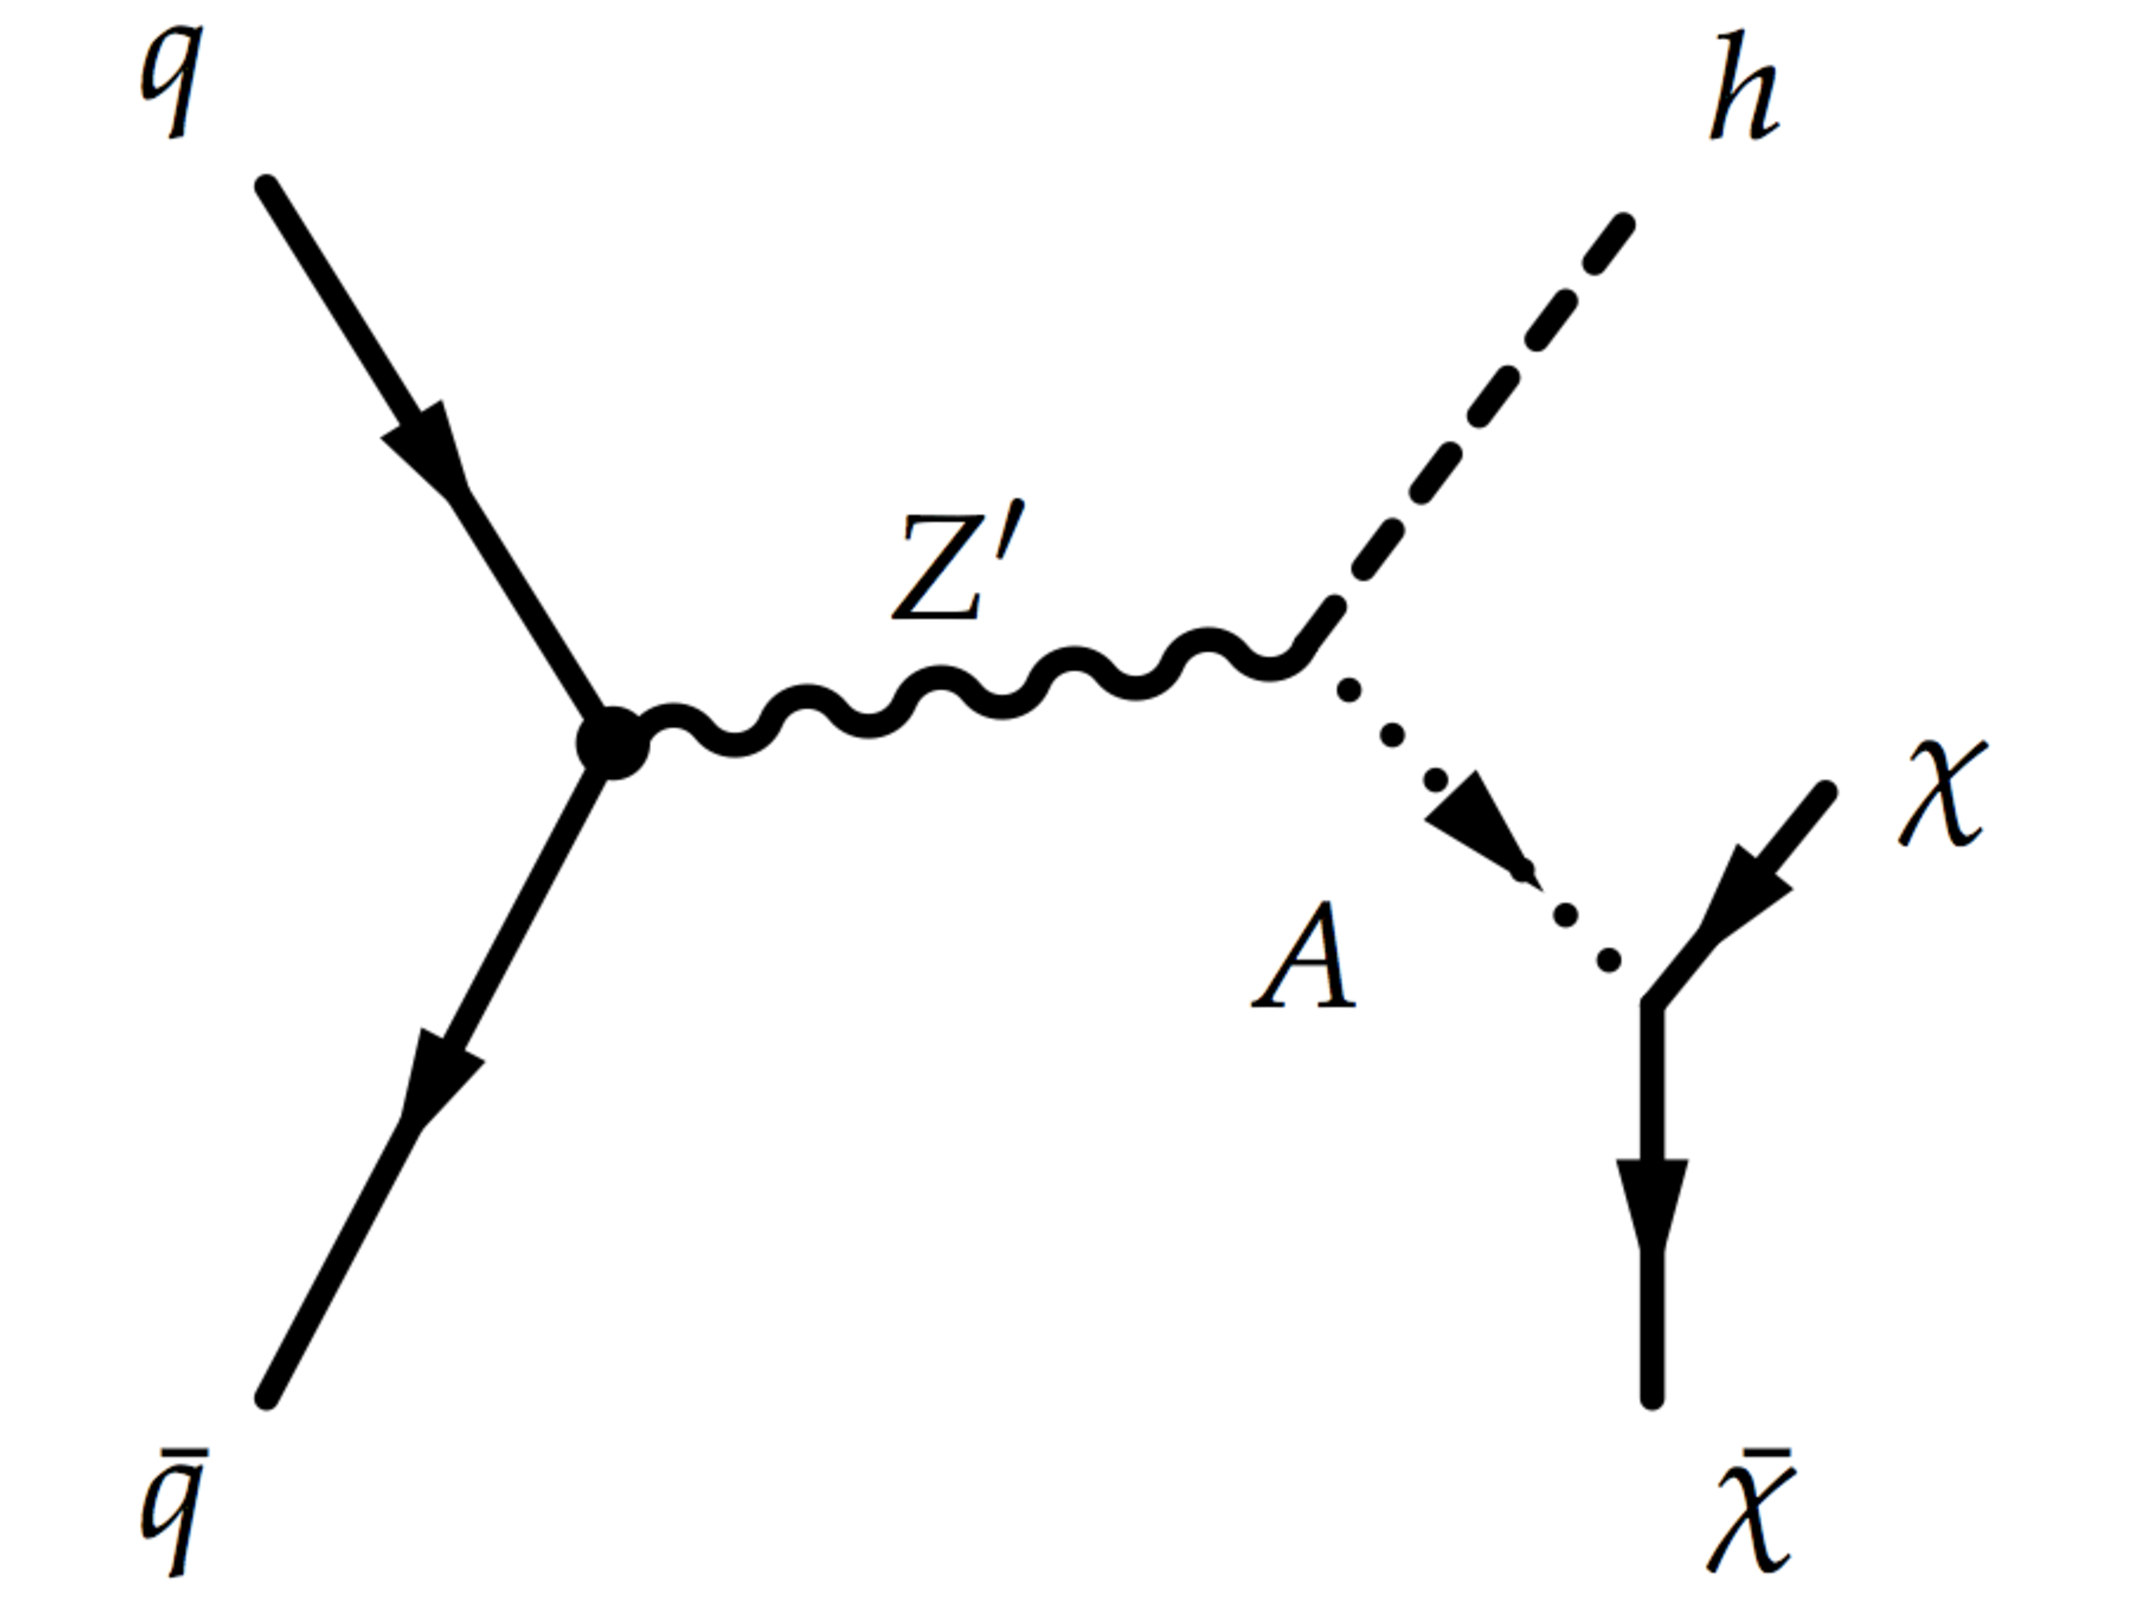
\includegraphics[width=0.35\textwidth]{Figure_001.pdf}
\caption{Leading order Feynman diagram of the \cPZpr-2HDM ``simplified model''. A pseudoscalar boson \Az decaying into invisible dark matter is produced from 
the decay of an on-shell $\cPZpr$ resonance. This gives rise to a Higgs boson 
and missing transverse momentum.}
\label{fig:feynman}
\end{figure}

In the \cPZpr-2HDM model, the gauge symmetry of the SM is extended by a
$U(1)_{\cPZpr}$ group, with a new massive \cPZpr\ gauge boson.
A Type-2 2HDM~\cite{Lee:1973iz,Branco:2011iw} is used to formulate 
the extended Higgs sector.
A doublet $\Phi_u$ couples only to up-type quarks, and 
a doublet $\Phi_d$ couples to down-type
quarks and leptons. 
Only $\Phi_u$ and right-handed up-type quarks $u_R$ have an associated charge 
under the $U(1)_{\cPZpr}$ group, while $\Phi_d$ and all other SM
fermions are neutral. 
After electroweak symmetry breaking, the Higgs doublets attain vacuum 
expectation values $v_u$ and $v_d$, 
resulting in five physical Higgs bosons: 
a light neutral CP-even scalar \Ph, assumed to be the 
observed 125\GeV Higgs boson, a heavy neutral CP-even scalar \PH,
a neutral CP-odd scalar \Az, and two charged scalars \Hpm.  
The analysis is performed in the context of the so-called 
alignment limit where the \Ph\ has SM-like couplings to fermions and gauge
bosons, and the ratio of the vacuum expectation values $\tan \beta = v_u/v_d > 0.3$, as implied from the perturbativity limit of the Yukawa 
coupling~\cite{2HDM,Craig:2013hca} of the top quark, the \Ph-\PH mixing angle $\alpha$ is 
related to $\beta$ by $\alpha = \beta - \pi/2$. 

The benchmark model is parametrized through six quantities: (i) the 
pseudoscalar mass 
\maz, (ii) the DM mass $m_{\chi}$, (iii) the \cPZpr\ mass \mzp,
(iv) $\tan \beta$, (v) the \cPZpr\ coupling strength \gzp, and (vi) 
the coupling constant between the \Az and DM particles $g_{\chi}$. 

Only the masses \maz and \mzp affect the kinematic 
distributions of the objects in the final states studied in this analysis. 
In fact, when \Az is on-shell, i.e. $\maz > 2 m_{\chi}$, the distributions 
have little dependence on $m_{\chi}$. 
The remaining parameters modify the cross section, branching fraction, and decay 
widths of the $\cPZpr$ and the \Az, resulting in only small changes to the 
final-state kinematic distributions. 

We consider a \cPZpr\ resonance with mass between 600 and 2500\GeV and 
an \Az with mass between 300 and 800\GeV, while the mass of DM particles $m_{\chi}$ is less than or equal to 100 GeV.
The parameters $\tan \beta$ and $g_{\chi}$ are fixed at unity and two different assumptions on \gzp\ are 
evaluated as described in more detail later. 
Values of \maz below 300\GeV are excluded by constraints on flavor changing 
neutral currents from measurements of $\cPqb\rightarrow \cPqs\gamma$ \cite{Branco:2011iw}, 
and are not considered here. 

The branching fraction for decays of \Az to DM particles, 
${\cal B}(\Az\rightarrow\chi\overline{\chi})$, decreases as $m_{\chi}$ 
increases;                                   
for the range of \maz considered here, the relative decrease of 
${\cal B}(\Az\rightarrow\chi\overline{\chi})$ is less than 7\% as $m_{\chi}$                              
increases from 0 to 100\GeV. 
Therefore, although signals with $m_{\chi}= 100\GeV$ are considered in this search, 
the results are valid for any value of dark matter mass below 100 \GeV.

With the assumed dark matter mass, the value of ${\cal B}(\Az\rightarrow\chi\overline{\chi})$ is ${\approx} 100\%$ for $\maz = 300\GeV$. 
The branching fraction starts to decrease for $\maz$ greater than twice the mass 
of the top quark as the decay $\Az\rightarrow$ $\cPqt\cPaqt$ becomes kinematically 
accessible. For example, if $\maz = 400~(800)\GeV$, ${\cal B}(\Az\rightarrow\chi\overline{\chi})$ 
reduces to $54~(42)\%$. The results presented here consider only \Az decays to 
DM particles and the signal cross section includes 
the value of ${\cal B}(\Az\rightarrow\chi\overline{\chi})$.

The quantity \ptvecmiss, calculated as the negative vectorial sum of the transverse momentum (\pt) of all objects identified in an event, represents the total
momentum carried by the DM particles. 
The magnitude of this vector is referred to as \MET.  
For a given value of \mzp, the \pt of the \Az decreases as \maz increases. 
Therefore, the \MET spectrum softens with increasing \maz. 
A comparison of the \MET distributions for three values of \maz is shown in Fig.~\ref{fig:mA0}. 

\begin{figure}[htbp]
\centering
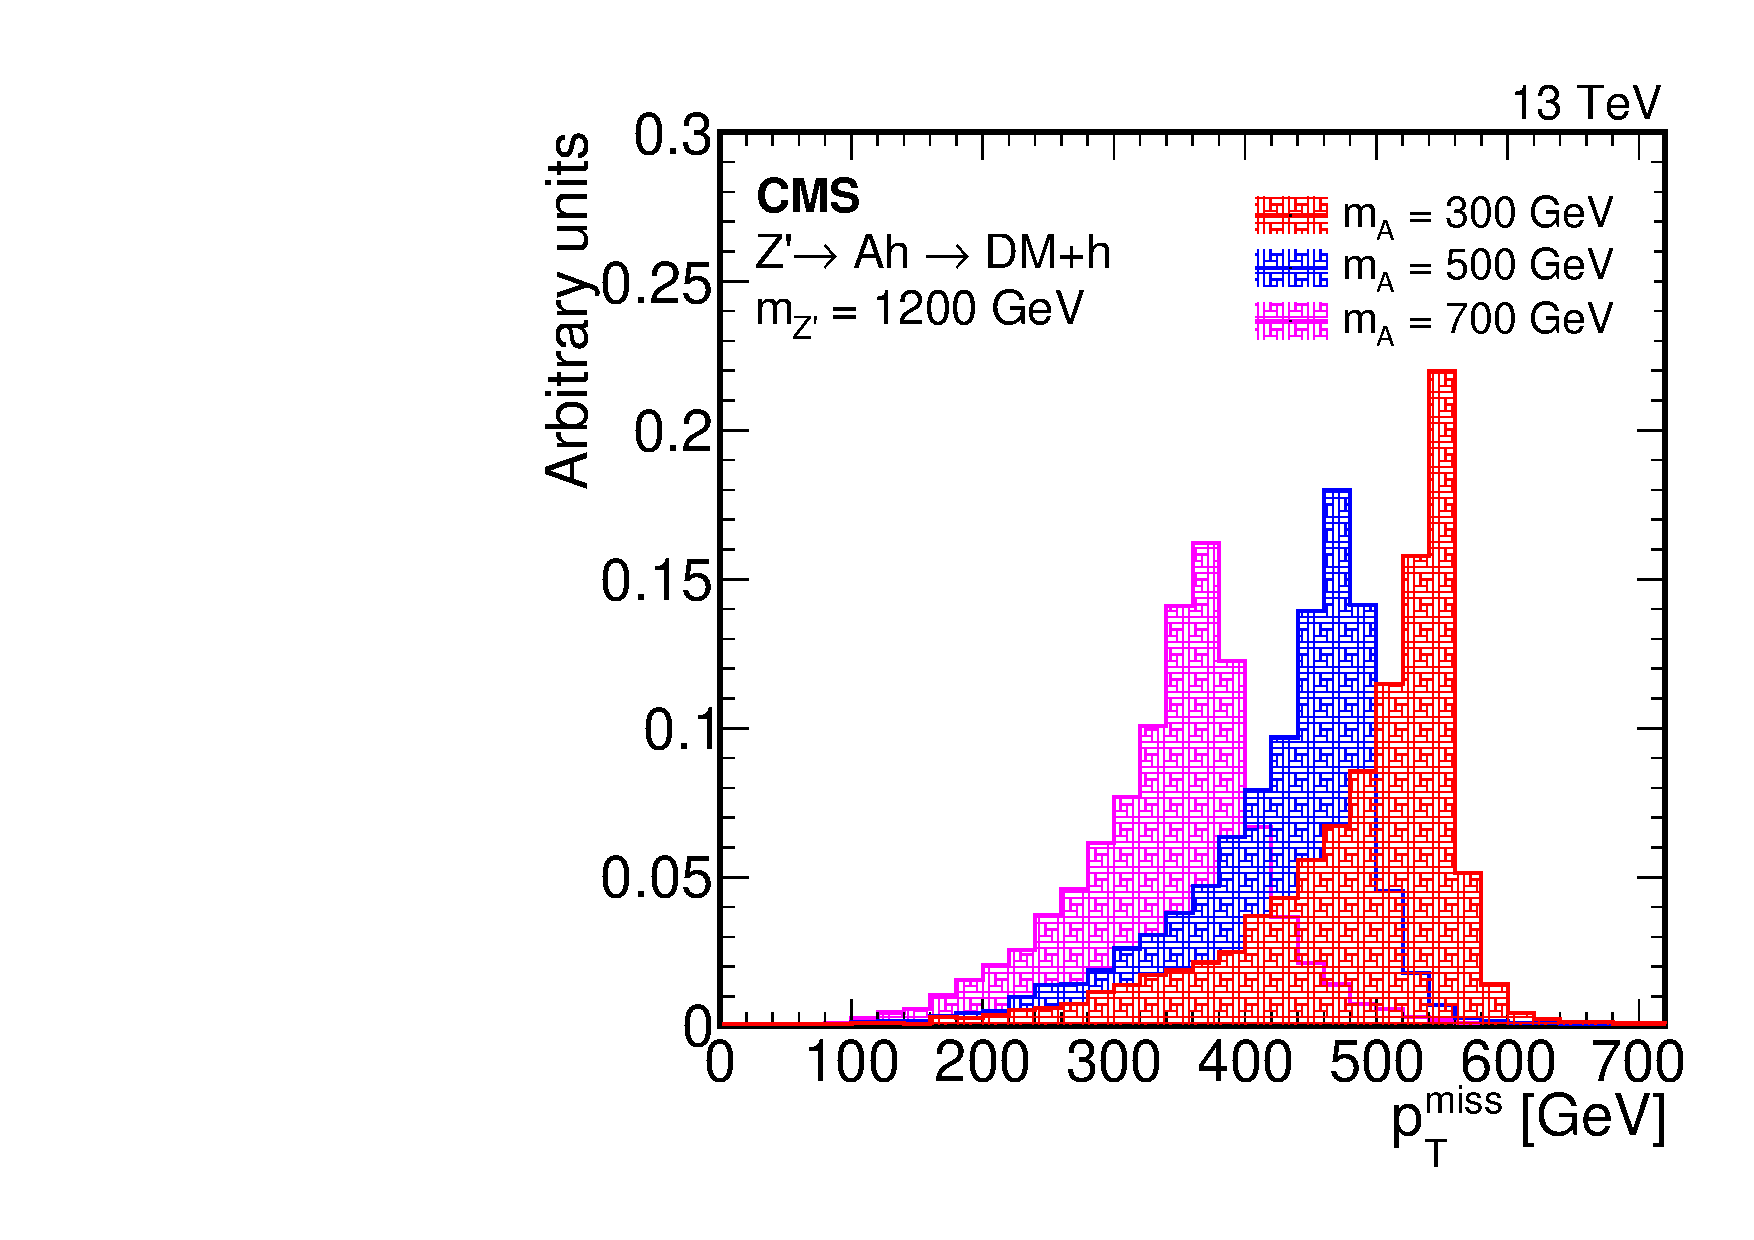
\includegraphics[width=0.45\textwidth]{Figure_002.pdf}
\caption{Distribution of \MET at generator level for \cPZpr\ $\rightarrow$ \Az~h $\rightarrow$ DM+h with \maz = 300, 500, and 700\GeV with \mzp = 1200\GeV. All other parameters of the model are fixed, as mentioned in the text.}
\label{fig:mA0}
\end{figure}

The signal cross section times branching fraction is calculated 
for two assumptions on \gzp: 
(i) a fixed value of \gzp = 0.8, as considered in Ref.~\cite{ATLAS-2015-PAS} and recommended in 
Ref.~\cite{Abercrombie:2015wmb}, 
and (ii) using the maximum value from electroweak global fits and 
constraints from dijet searches~\cite{2HDM,private}:
\begin{equation}
\label{eq:gz}
\gzp = 0.03\, \frac{g_{\mathrm{W}}}{\cos\theta_{W}\sin^{2}\beta} \, \frac{\sqrt{m_{\mathrm{Z'}}^{2}-m_{\mathrm{Z}}^{2}}}{m_{\mathrm{Z}}}, 
\end{equation} 
yielding $\gzp=0.485$ for $\mzp=1\TeV$, and $\gzp=0.974$ for $\mzp=2\TeV$. 
It can be seen from Eq.~\ref{eq:gz} that \gzp = 0.8 is the maximum allowed value of \gzp\ for 
$\tan \beta=1$ and \mzp=1.7~\TeV (the best reach of LHC as estimated by Ref.~\cite{2HDM}).  
Note that this analysis does not consider the contribution of another decay that gives a similar mono-h 
signature, $\cPZpr\rightarrow \cPZ \mathrm{h}$ where $\cPZ\rightarrow\nu\overline{\nu}$. 
The ratio of branching fractions, 
${\cal B}(\cPZpr\rightarrow \cPZ \mathrm{h},\cPZ\rightarrow\nu\overline{\nu})/{\cal B}(\cPZpr \rightarrow \Az \mathrm{h},\Az\rightarrow\chi\overline{\chi})$, 
is a function of $\tan \beta$ and \mzp and does not depend on \gzp since 
the value of \gzp cancels in the ratio.


The \Hbb  decay mode has the largest branching fraction (${\approx} 58 \%$) of all, but suffers from relatively poor mass resolution of about 10\%, and while the \HGG branching fraction is small (${\approx} 0.2\%$), the channel benefits from the high precision in reconstructed diphoton mass, with a resolution of about 1--2\%.

\par In the \Hbb channel, the fact that 
the \pt of the \Ph\ should increase with \mzp and 
decrease with \maz is exploited.  
The minimum separation in the pseudorapidity and azimuth ($\eta$, $\phi$) plane
between the decay products of h scales as $m_{\Ph}/p_{\mathrm{T}}^{\mathrm{h}}$, where 
$p_{\mathrm{T}}^{\mathrm{h}}$ is the transverse momentum of the h boson.  
The allowed mass ranges of \mzp and \maz
imply a very wide range of values for $p_{\mathrm{T}}^{\mathrm{h}}$ 
and consequently a wide range in the separation of the decay products.
Analysis in this channel is therefore divided into two regimes: (i) a 
resolved regime where the \Ph decays to two distinctly reconstructed b jets, %using a distance parameters of  0.4, 
%and (ii) a Lorentz-boosted regime where the \Ph is reconstructed as a single jet with a distance parameter 0.8. 
and (ii) as a single fat jet. 
For each mass point, the analysis with best sensitivity for the expected limit is used as the final result. 
The signal extraction is performed through a simultaneous fit to the signal- and background-enriched 
control regions.  

The search in the \HGG channel is performed by seeking an excess of events 
over the SM prediction in the diphoton mass spectrum, after requiring a large 
\MET. 
Control samples in data are used to estimate the reducible background, which 
mainly consists of diphoton SM production. A counting approach is used 
to estimate the potential signal. 

\subsection{Event selection and background estimation}\label{sec:eventselection}
\label{eventselection}

This analysis searches for excesses over the background-only prediction in events with large \MET and a system of two b-tagged jets or two photons that has a reconstructed invariant mass close to the mass of the SM-like Higgs boson \Ph. 
In the \Hbb decay channel, the analysis relies on fitting the \MET distribution simultaneously in the signal region (SR), defined after selecting a mass window around the Higgs boson mass, and in background-enriched control regions (CRs). 
For the \HGG decay channel, a simple analysis is performed where the signal and resonant background contributions are estimated by counting 
the number of simulated events in the SR, while the nonresonant background is
extrapolated from the data in a low-\MET region. 
In the following sections, the event selection and analysis strategy are described in detail for the \Hbb channel only.

A search for DM produced in association with \Hbb is performed in a resolved regime, where events are required to have at least two AK4 jets, and in the 
Lorentz-boosted regime where one AK8 jet is required. 
In addition, \MET is required to be large because it is a key signature of the signal events
and it provides strong rejection against the large reducible backgrounds. 

\subsubsection{Event selection}
The trigger used in the selection of signal-like events requires $\MET > 90\GeV$ and $H_{\mathrm{T}}^{\mathrm{miss}} > 90\GeV$, where $H_{\mathrm{T}}^{\mathrm{miss}}$ is defined as the magnitude of the vectorial sum of the \pt of all jets in the event with $p_{\mathrm{T}} > 20\GeV$. 
An additional trigger with a $\MET > 170\GeV$ requirement is used to achieve higher efficiency.
In this way, events with either high \MET or high $H_{\mathrm{T}}^{\mathrm{miss}}$ will pass the trigger.
For events passing the selection criteria that have $ \MET > 170 (200)\GeV$ for the resolved (boosted) analysis, the trigger efficiency is found to be greater than 98\%. 
%The \MET threshold for the resolved analysis is slightly lower to enhance the signal efficiency in the phase space that has a softer \MET distribution.
The \MET threshold for the resolved analysis is set slightly lower to enhance the signal efficiency in this region of phase space, where the \MET distribution is softer.

%Event filters \cite{CMS-PAS-JME-16-004} are used to remove detector induced (noise in ECAL or HCAL, or beam halo) high \MET events. 
%It has been verified that the efficiency of these filter on signal events is more than 99.99\%.
Event filters are used to remove spurious high \MET events caused by instrumental noise in the calorimeters or beam halo muons. It has been verified that the efficiency of these filters for accepting signal events is more than 99.99\%.
%It has been verified that the filters \cite{CMS-PAS-JME-16-004} used to remove instrumental background events, which produce high mismeasured \MET, do not reduce the signal efficiency. 
The main part of the event selection consists of Higgs boson tagging. This selection is different for the resolved and boosted analyses.
In the resolved regime, events are 
required to have two AK4 jets with $\pt>30\GeV$ and $|\eta|< 2.4$. 
These two jets are used to reconstruct the Higgs boson candidate, which 
is required to have $\pt > 150\GeV$.
Each of the two AK4 jets in the resolved regime is required to pass the b tagging selection, whereas in the boosted regime, the two subjets inside an AK8 jet must both pass the b tagging selection. 
In the boosted regime, the decay products from the Higgs boson are merged. Therefore, an AK8 jet with \pt greater than 200\GeV is used to reconstruct 
the Higgs boson. If more than one Higgs boson candidate is reconstructed, the ambiguity is resolved by selecting the candidate with the highest \pt. 
Backgrounds due to hadronic jets are further reduced by constraining the reconstructed Higgs boson candidate mass, $m_\mathrm{bb}$, to be between 100 and 150\GeV.
%For the resolved regime, Higgs boson candidate mass is reconstructed using two b, to be between 100 and 150\GeV. 
For the resolved regime, the Higgs boson candidate mass is reconstructed using two b-tagged AK4 jets. 
For the boosted regime, the corrected pruned mass of the AK8 jet with two b-tagged subjets is used as the Higgs boson candidate mass. 

Multijet events can act as a source of background  when the energy of one of the jets is mismeasured. 
Therefore, the absolute difference between the azimuthal angles of the vector 
\ptvecmiss\ and any other AK4 jet with $\pt > 30\GeV$ 
is required to be greater than 0.4 radians. 
Multijet background is further reduced in the 
resolved analysis by requiring the azimuthal angle difference between the \ptvecmiss and $\vec{p}_{\mathrm{\, T,trk}}^{\mathrm{\, miss}}$ to be less than 0.7 radians. 

Events are rejected if they have any  
isolated electron (muon) with $\pt > 10\GeV$ and $|\eta| < $ 2.5 (2.4) or any $\tau_\mathrm{h}$ candidates with $\pt > 20\GeV$ and $|\eta| < 2.3$~\cite{Khachatryan:2015hwa,Chatrchyan:2013sba,CMSTauJINST}. 
In addition, the events must not have any additional loose AK4 b-tagged jet or 
more than one additional AK4 jet with $\pt > 30\GeV$ and $|\eta| < 4.5$. 
These vetoes considerably reduce the background from semileptonic top decay 
modes and leptonic decays of W+jets. 

The product of the detector acceptance and selection efficiency varies from 
1 to 29\%, depending on the values of 
\mzp and \maz. The average \MET increases with \mzp and decreases with \maz. 
The overall selection efficiency, shown in Table \ref{tab:AcceptanceHGG}, 
%Therefore, the selection efficiency 
follows the same trend.

\subsubsection{Analysis strategy and background estimation}

Several CRs are used to 
correct the background normalizations with dedicated scale factors. For both resolved and boosted regimes, the selection criteria of these CRs are kept as close as possible to those of the SR, except for the inversion of the additional 
object vetoes (leptons, jets) and the Higgs boson mass window.
This makes the CRs orthogonal to the SR.

For the resolved regime, three CRs are specified: Z($\rightarrow\nu\overline{\nu}$)+jets, 
top quark, and W+jets.
The b tagging selection in all the CRs is the same as in the SR in order to minimize the b tagging systematic uncertainties
when extrapolating the background scale factors measured in the CRs to the SR. 
The Z($\rightarrow\nu\overline{\nu}$)+jets CR is defined with the same selection as the 
SR, except for the inversion of the reconstructed Higgs boson mass requirement. 
The W+jets and top quark CRs are defined by removing the mass selection and 
requiring exactly one isolated electron (muon) with $\pt > 10~\GeV$ and 
$|\eta|< 2.5$ (2.4). 
Events with one additional AK4 jet are placed in the top quark CR, whereas 
events with no additional AK4 jets enter the W+jets CR. 

For the boosted regime, the Z($\rightarrow\nu\overline{\nu}$)+jets CR is defined by inverting the mass requirement for the AK8 jet. 
Owing to the low event count and very similar topology between the W+jets and top 
quark backgrounds it is difficult to 
construct two separate CRs for W+jets and top quark backgrounds. 
Hence, the single-lepton CR, a combination of mainly W+jets and top quark 
events, is defined using the same selection as that for the signal, but 
requiring exactly one lepton and removing the mass requirement. 

Figure~\ref{fig:massHbb} shows the Higgs boson candidate mass for the resolved and boosted regimes.  They correspond to the 
simultaneous fit of the \MET distributions in the SR and background enriched CRs to extract the signal.
Data-to-simulation ratios for pre-fit and post-fit background predictions are shown in the lower panels of all Figs.~\ref{fig:massHbb}--\ref{fig:finalSignalPlots}.

\begin{figure}[htbp]
\centering
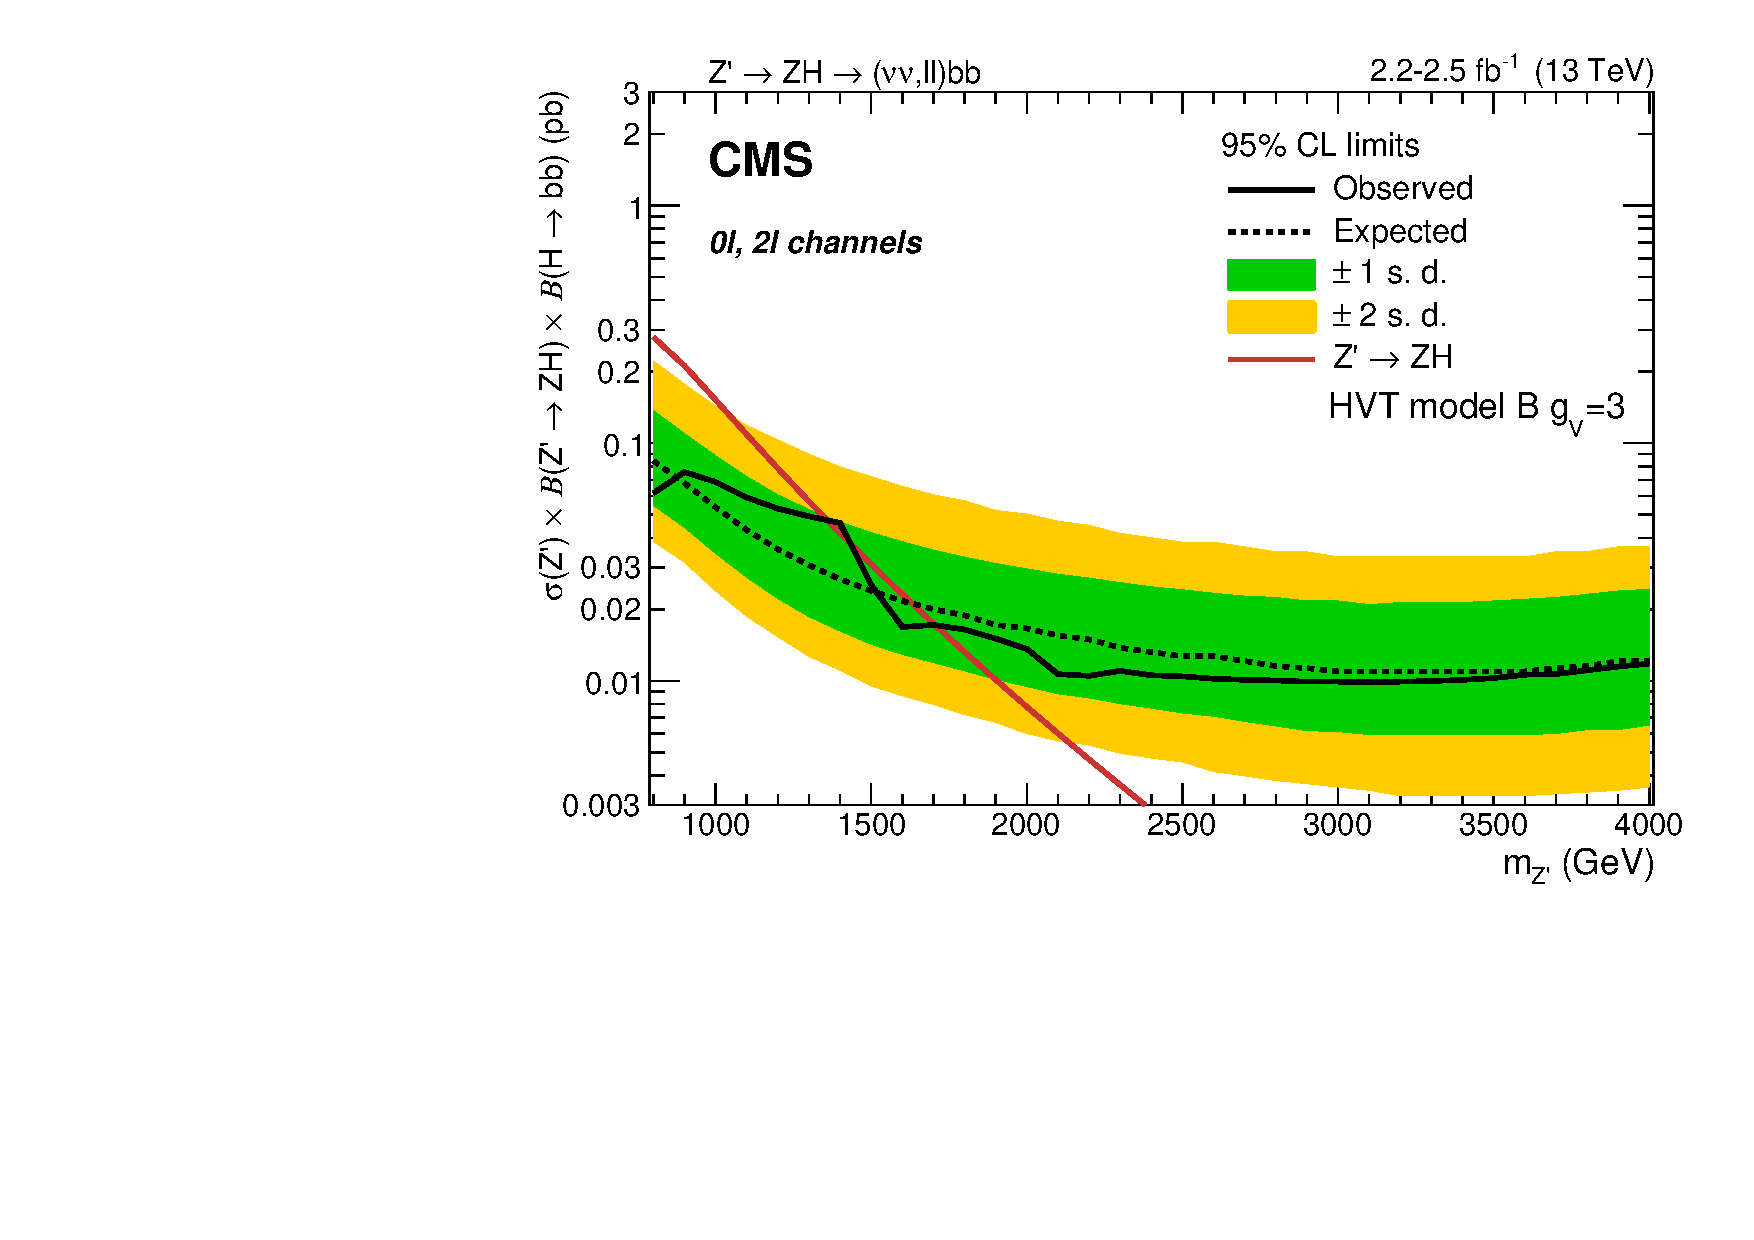
\includegraphics[width=0.45\textwidth]{Figure_003-a.pdf}
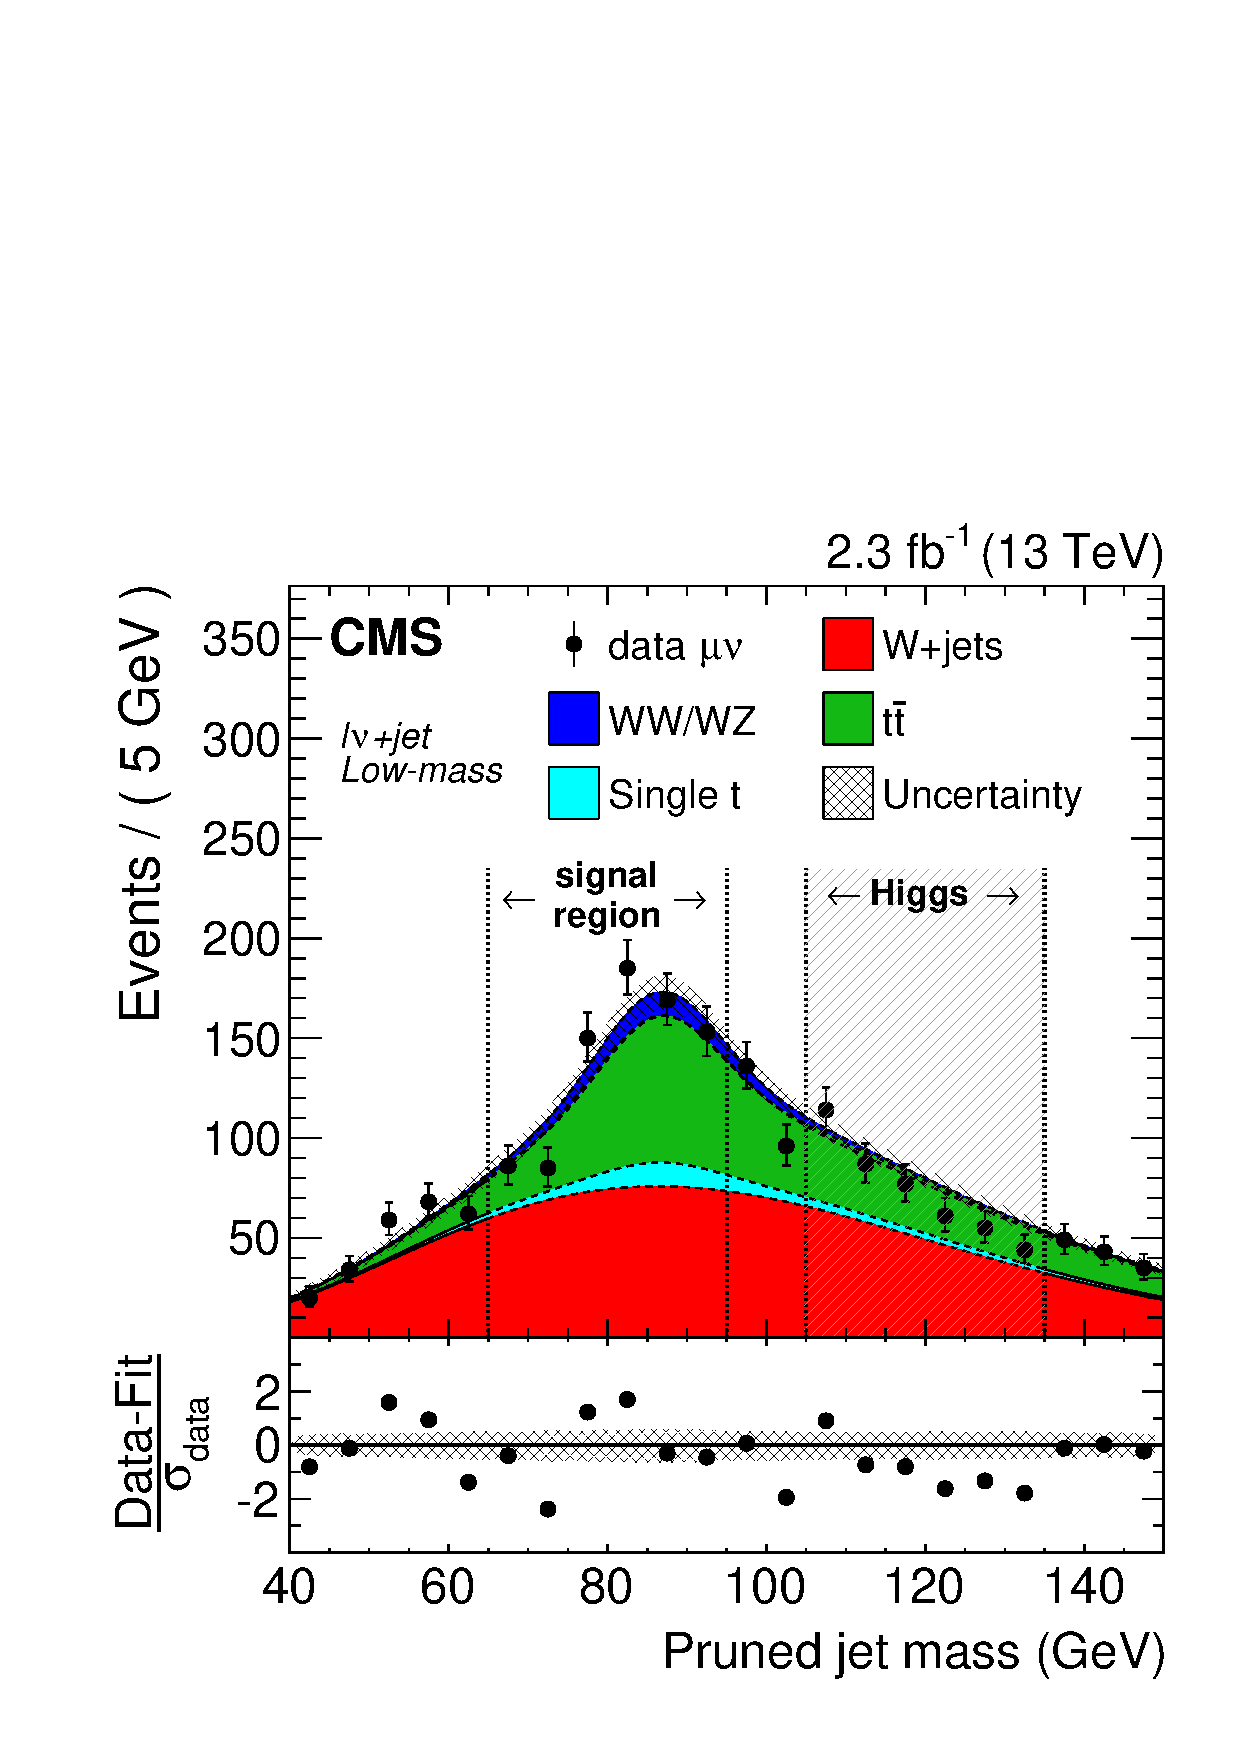
\includegraphics[width=0.45\textwidth]{Figure_003-b.pdf}
\caption{Post-fit distribution of the reconstructed Higgs boson candidate mass expected from SM backgrounds and observed in data for the resolved (left) 
and the boosted (right) regimes with three different \mzp signal points overlaid. Other parameters for this model are fixed to $m_{\chi} = 100\GeV$ and $\tan{\beta} = g_{\chi} = 1$. The cross sections times branching fractions for the signal models are computed assuming \gzp = 0.8. The bottom panels show the data-to-simulation ratios for pre-fit (red markers) and post-fit (black markers) background predictions with a hatched band corresponding to the uncertainty due to the finite size of simulated samples and a gray band that represents the systematic uncertainty in the post-fit background prediction. The second bin represents the SR, while the events in the first and third bins are merged and represent the mass sidebands (Z($\rightarrow\nu\overline{\nu}$)+jets) CR. }

\label{fig:massHbb}
\end{figure}

\begin{figure}[htbp]
\centering
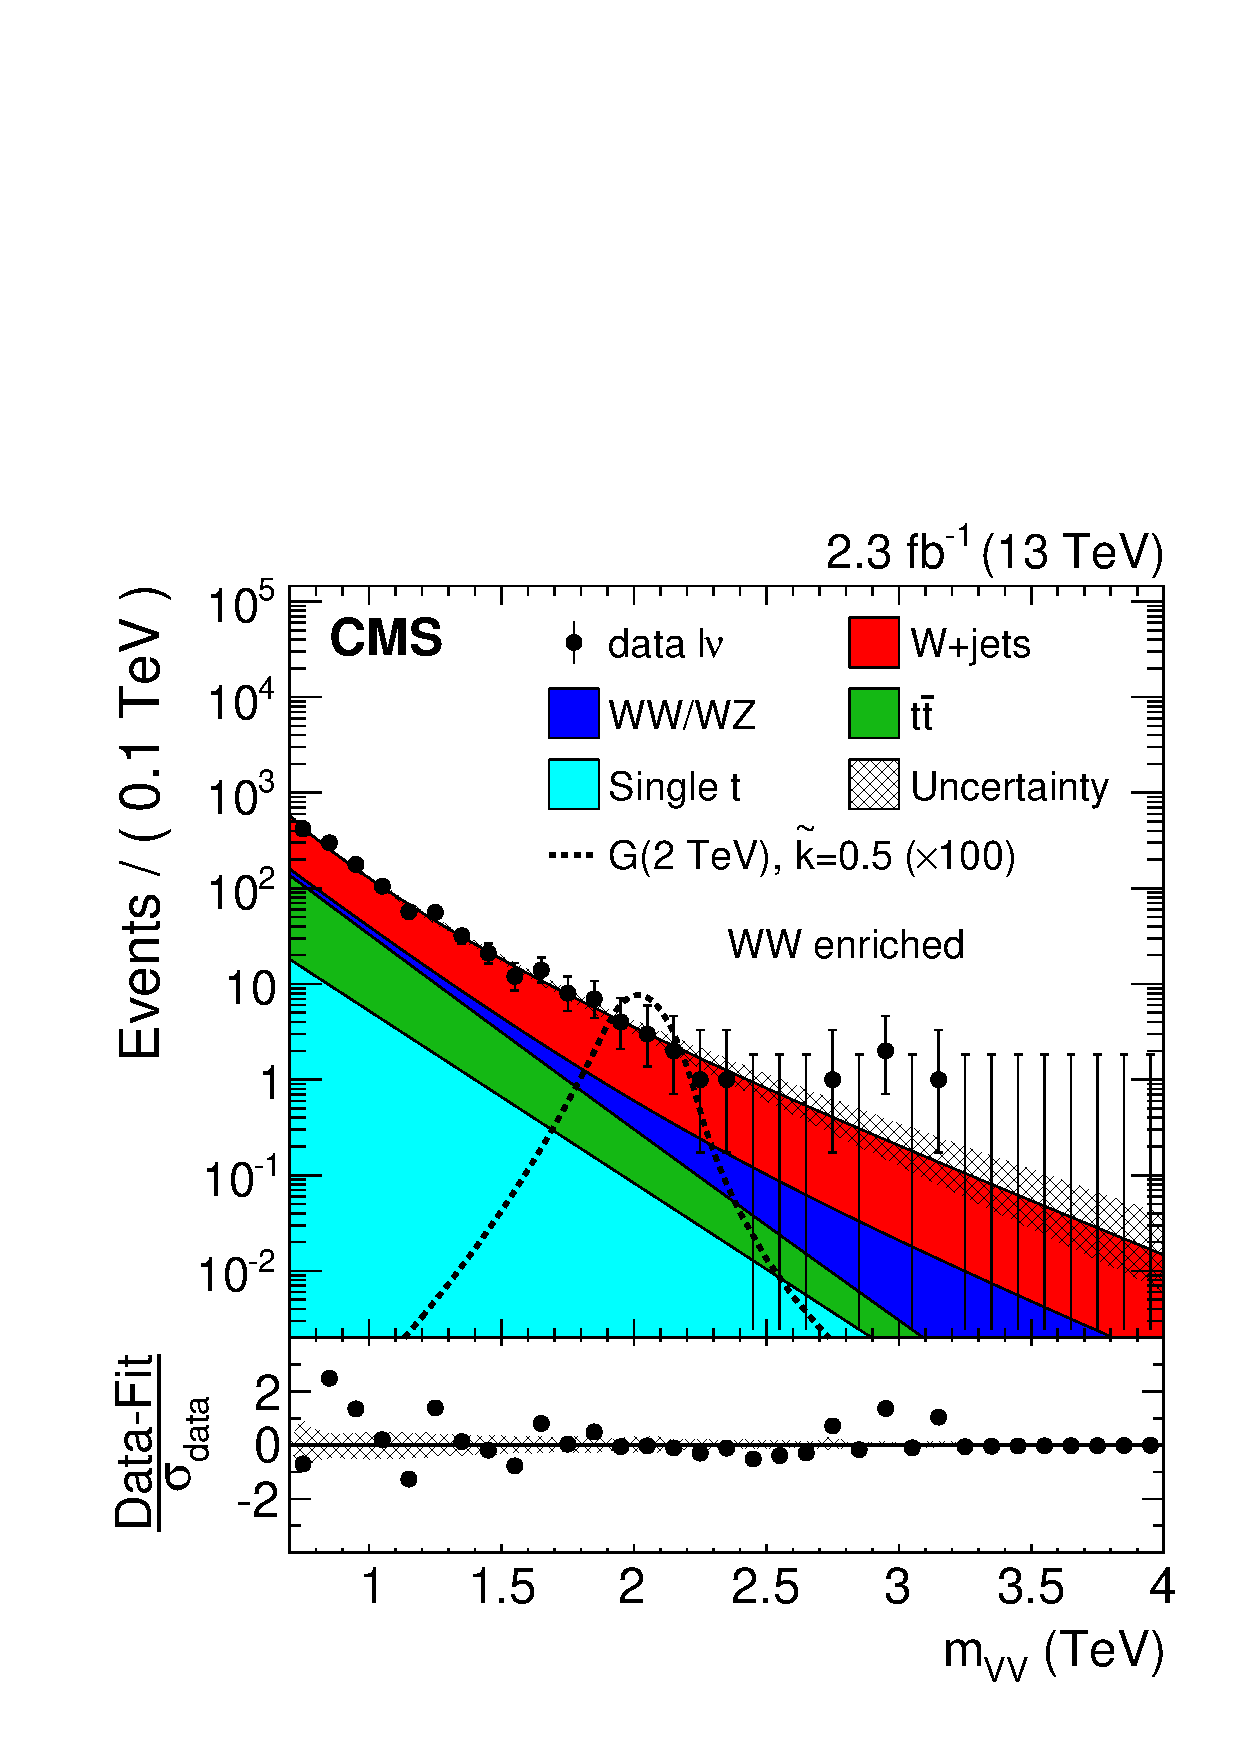
\includegraphics[width=0.49\textwidth]{Figure_004-a.pdf}
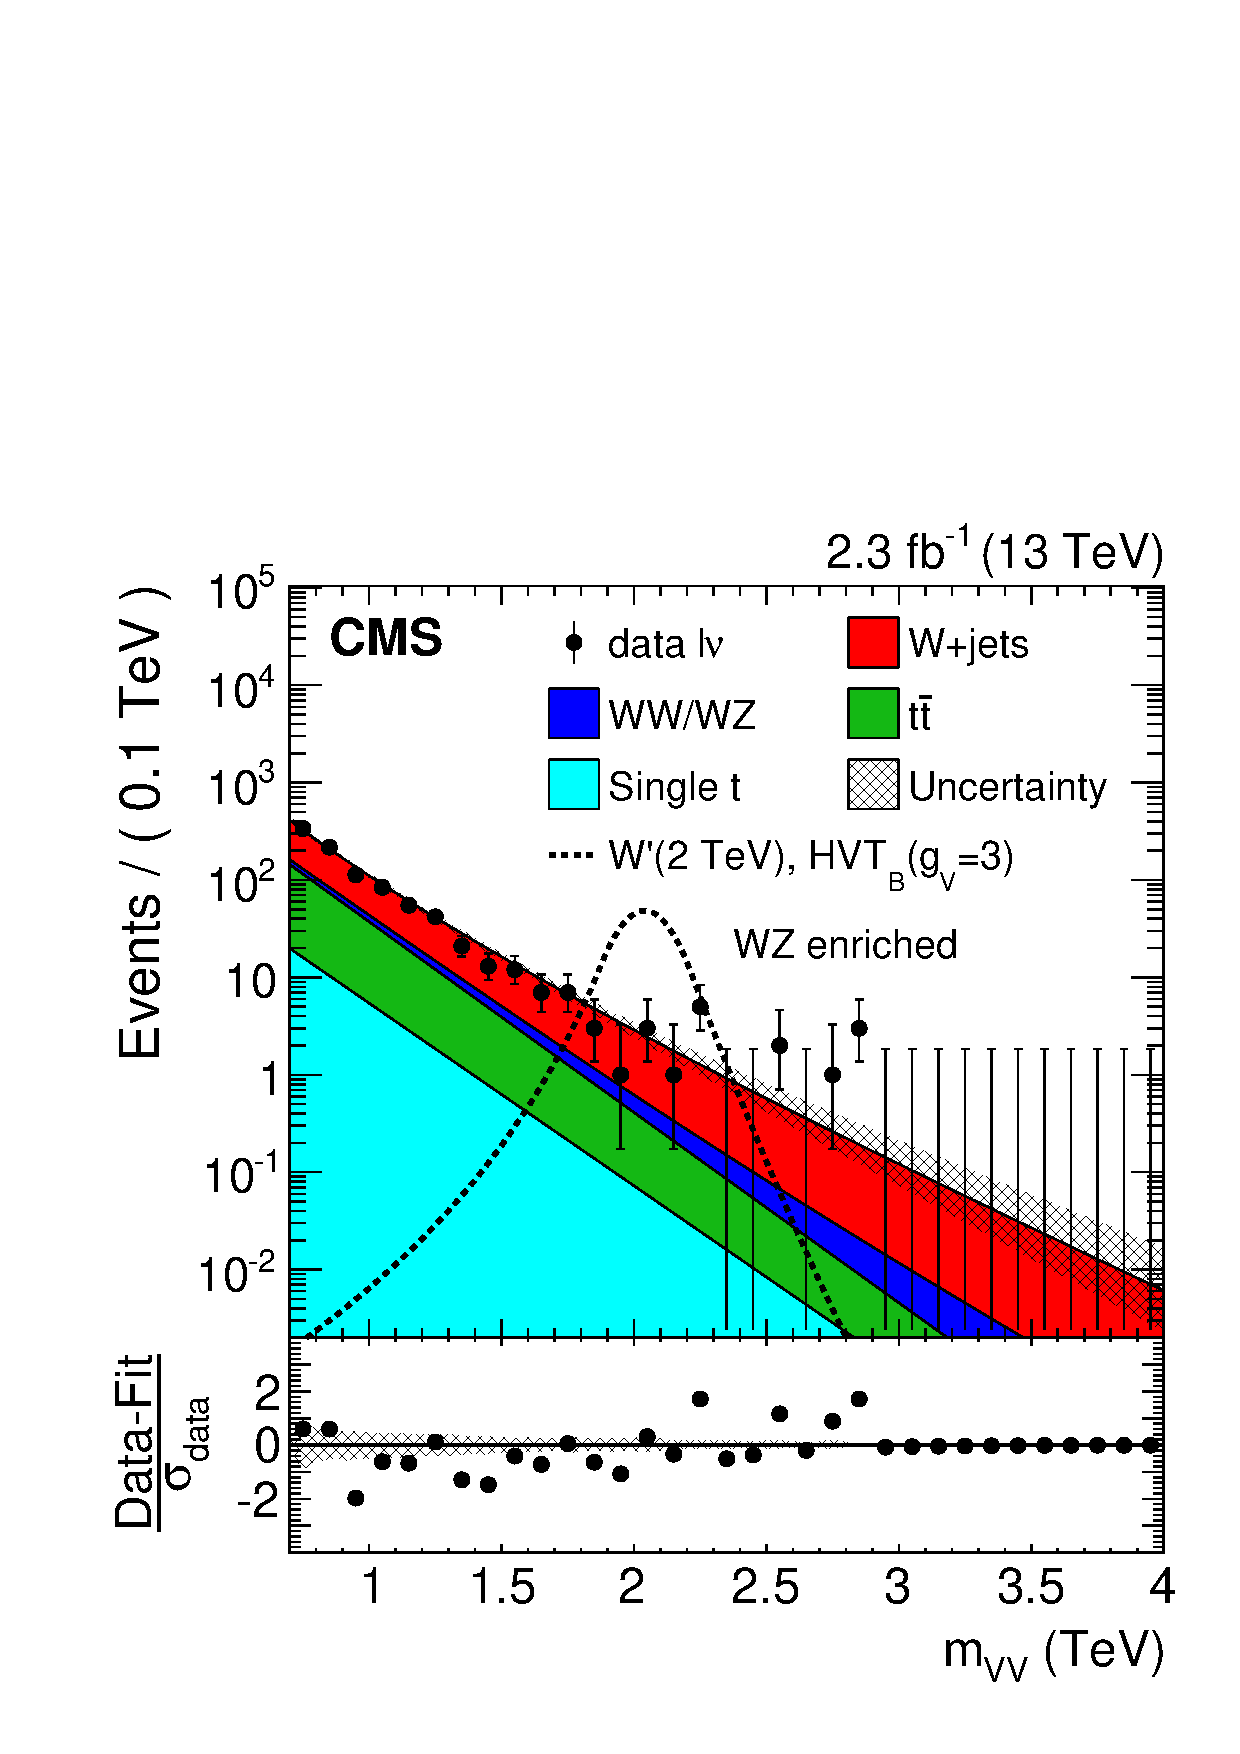
\includegraphics[width=0.49\textwidth]{Figure_004-b.pdf}
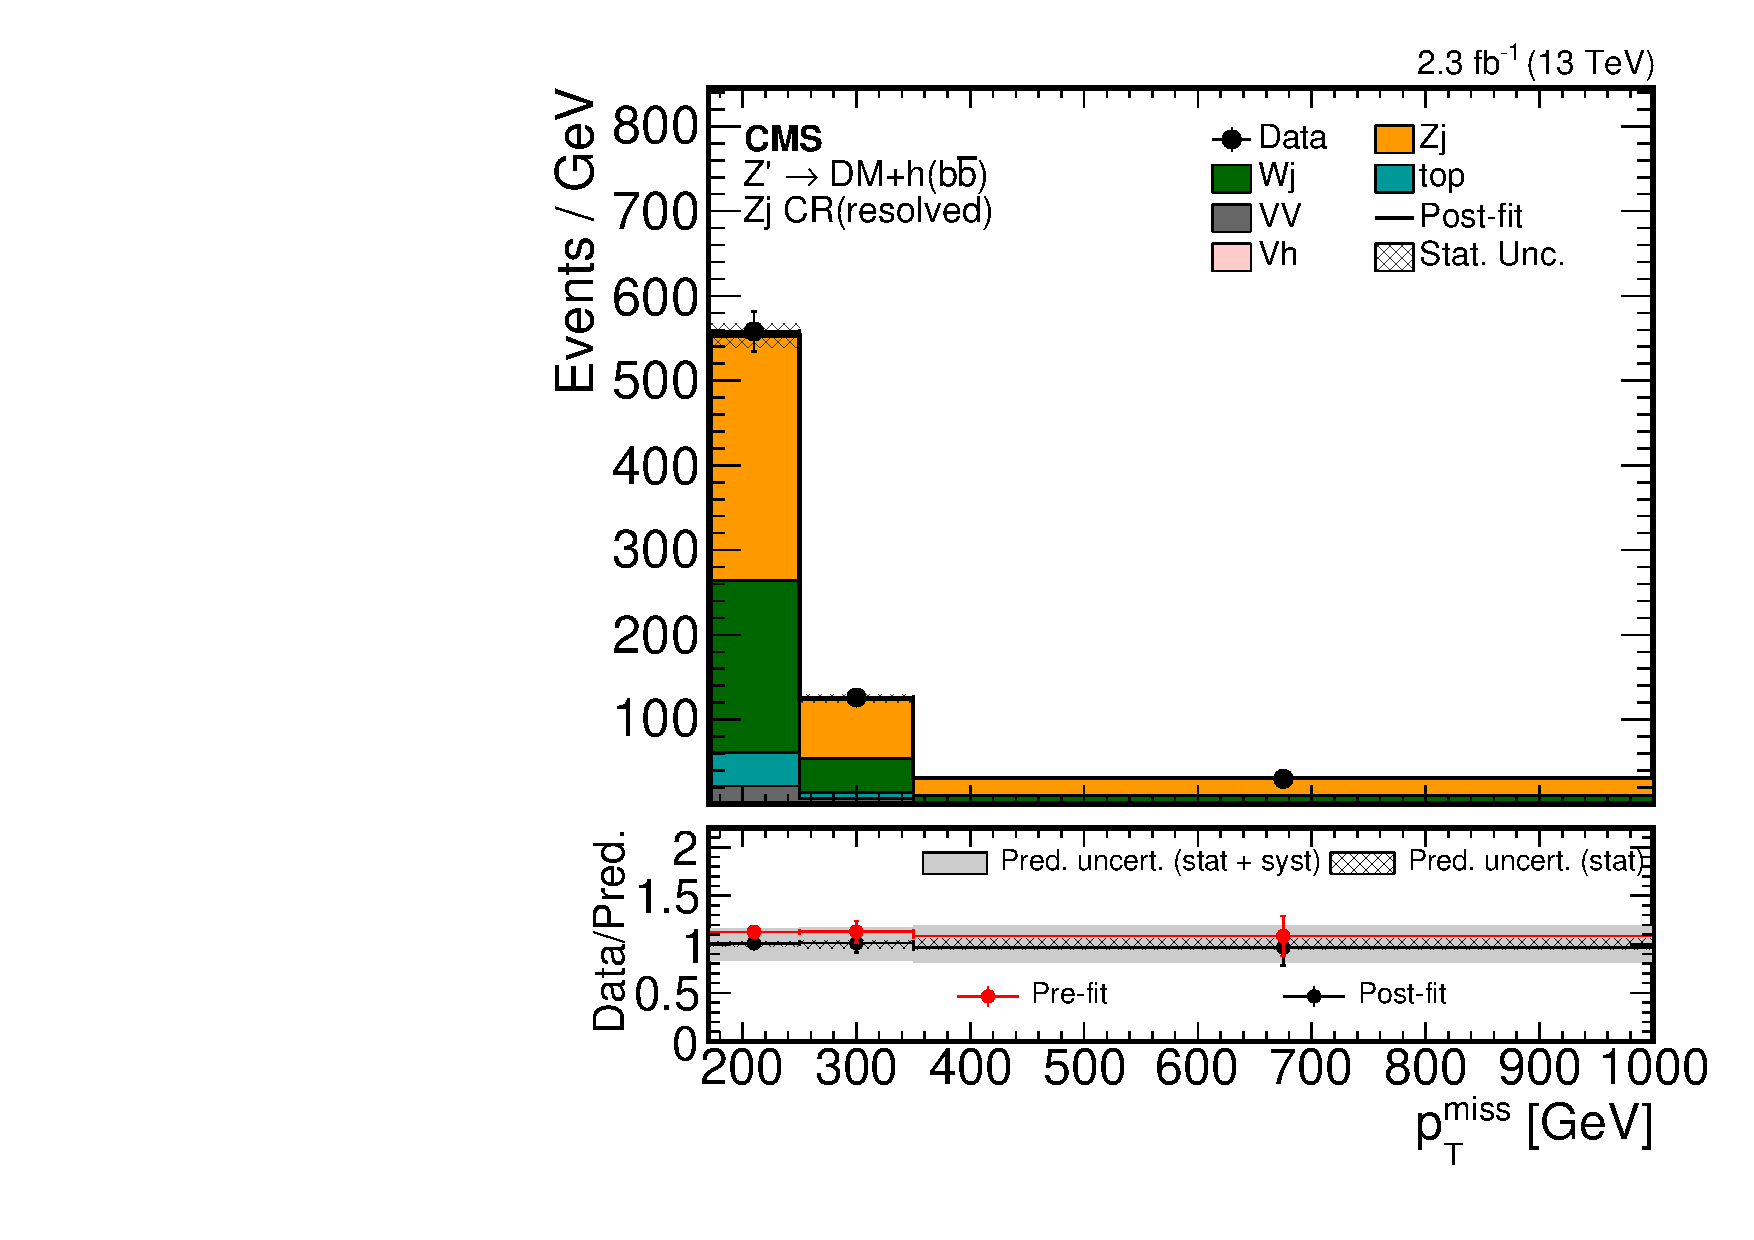
\includegraphics[width=0.49\textwidth]{Figure_004-c.pdf}

\caption{Post-fit distribution of \MET expected from SM backgrounds and observed in data for the W+jets (upper left), top quark (upper right) and Z($\rightarrow\nu\overline{\nu}$)+jets (lower) CRs for the resolved regime.  The bottom panels show the data-to-simulation ratios for pre-fit (red markers) and post-fit (black markers) background predictions with a hatched band corresponding to the uncertainty due to the finite size of simulated samples and a gray band that represents the systematic uncertainty in the post-fit background prediction. The last bin includes all events with $\MET > 350\GeV$.}
\label{fig:controlregionR}
\end{figure}

\begin{figure}[htbp]
\centering
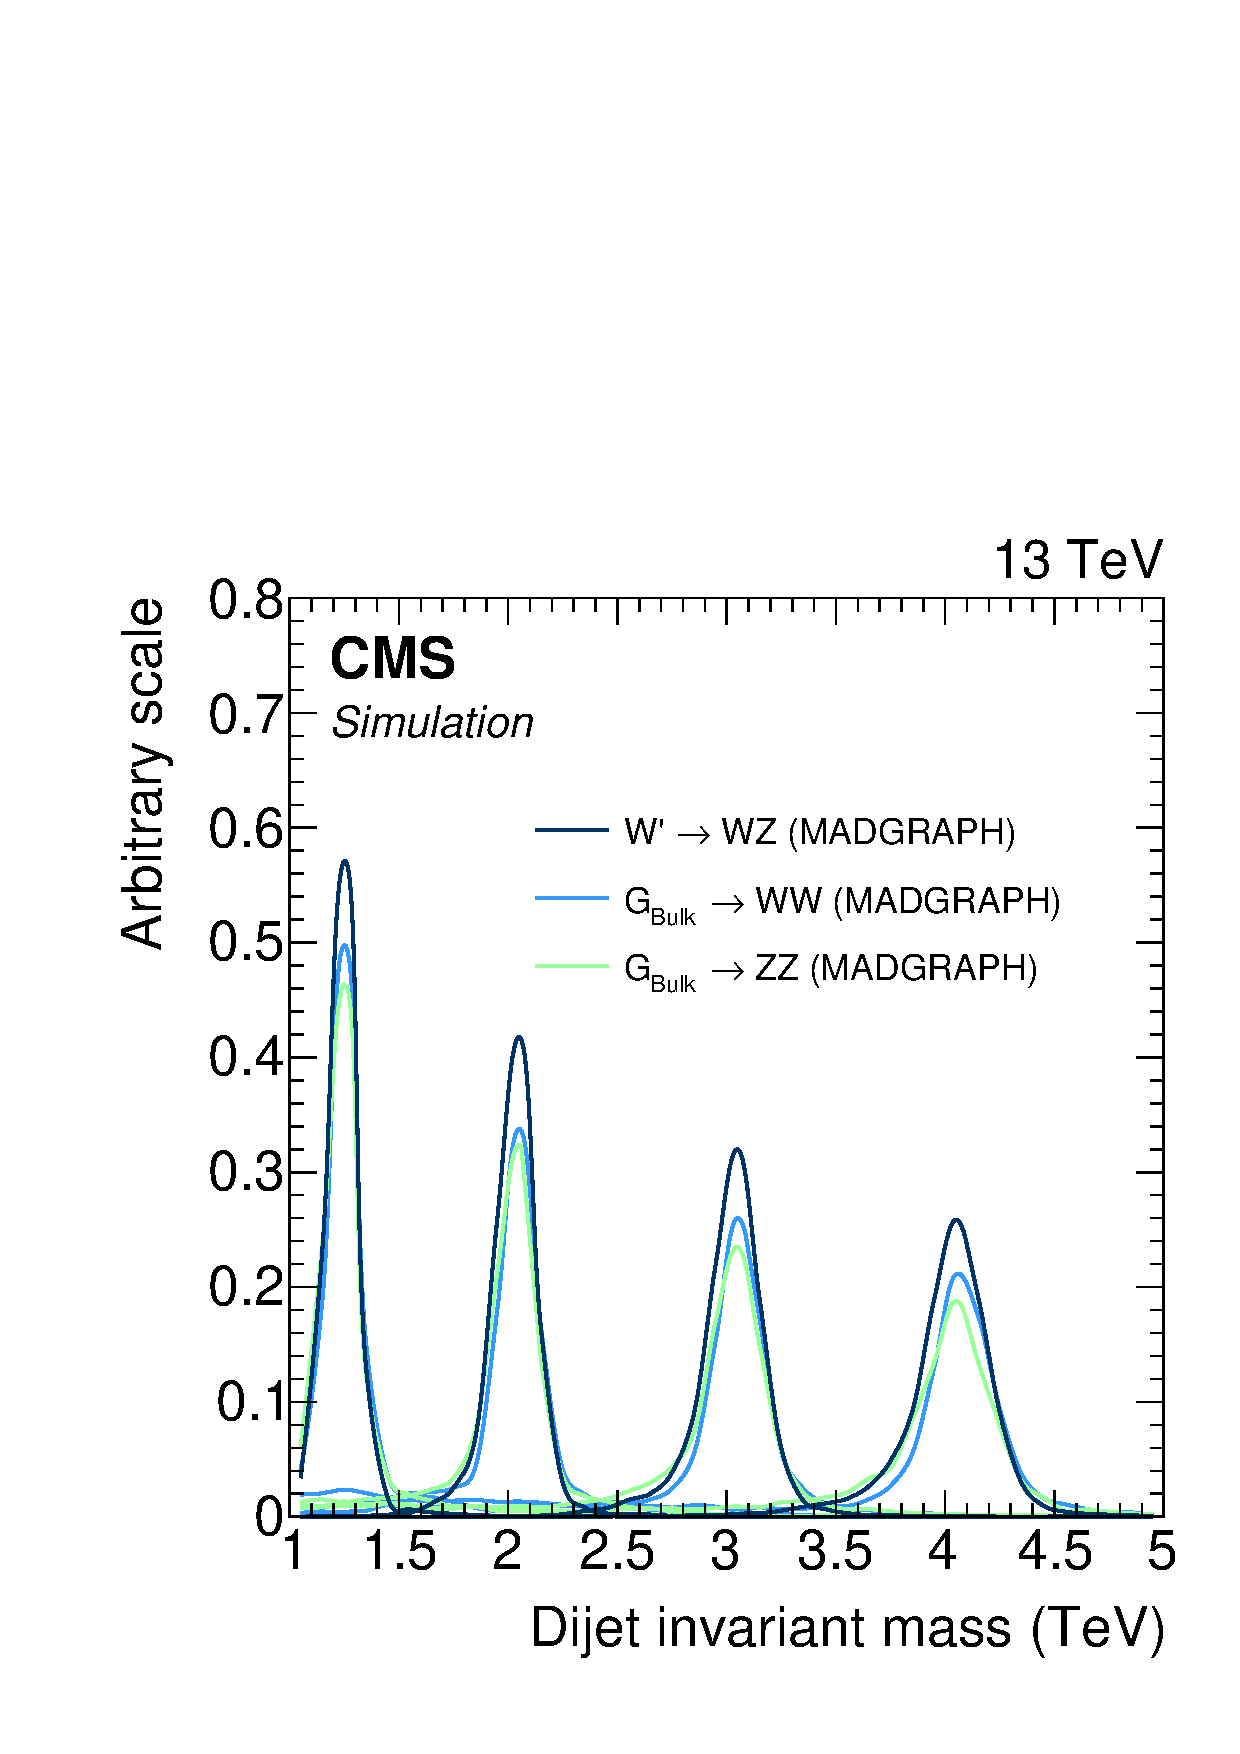
\includegraphics[width=0.49\textwidth]{Figure_005-a.pdf}
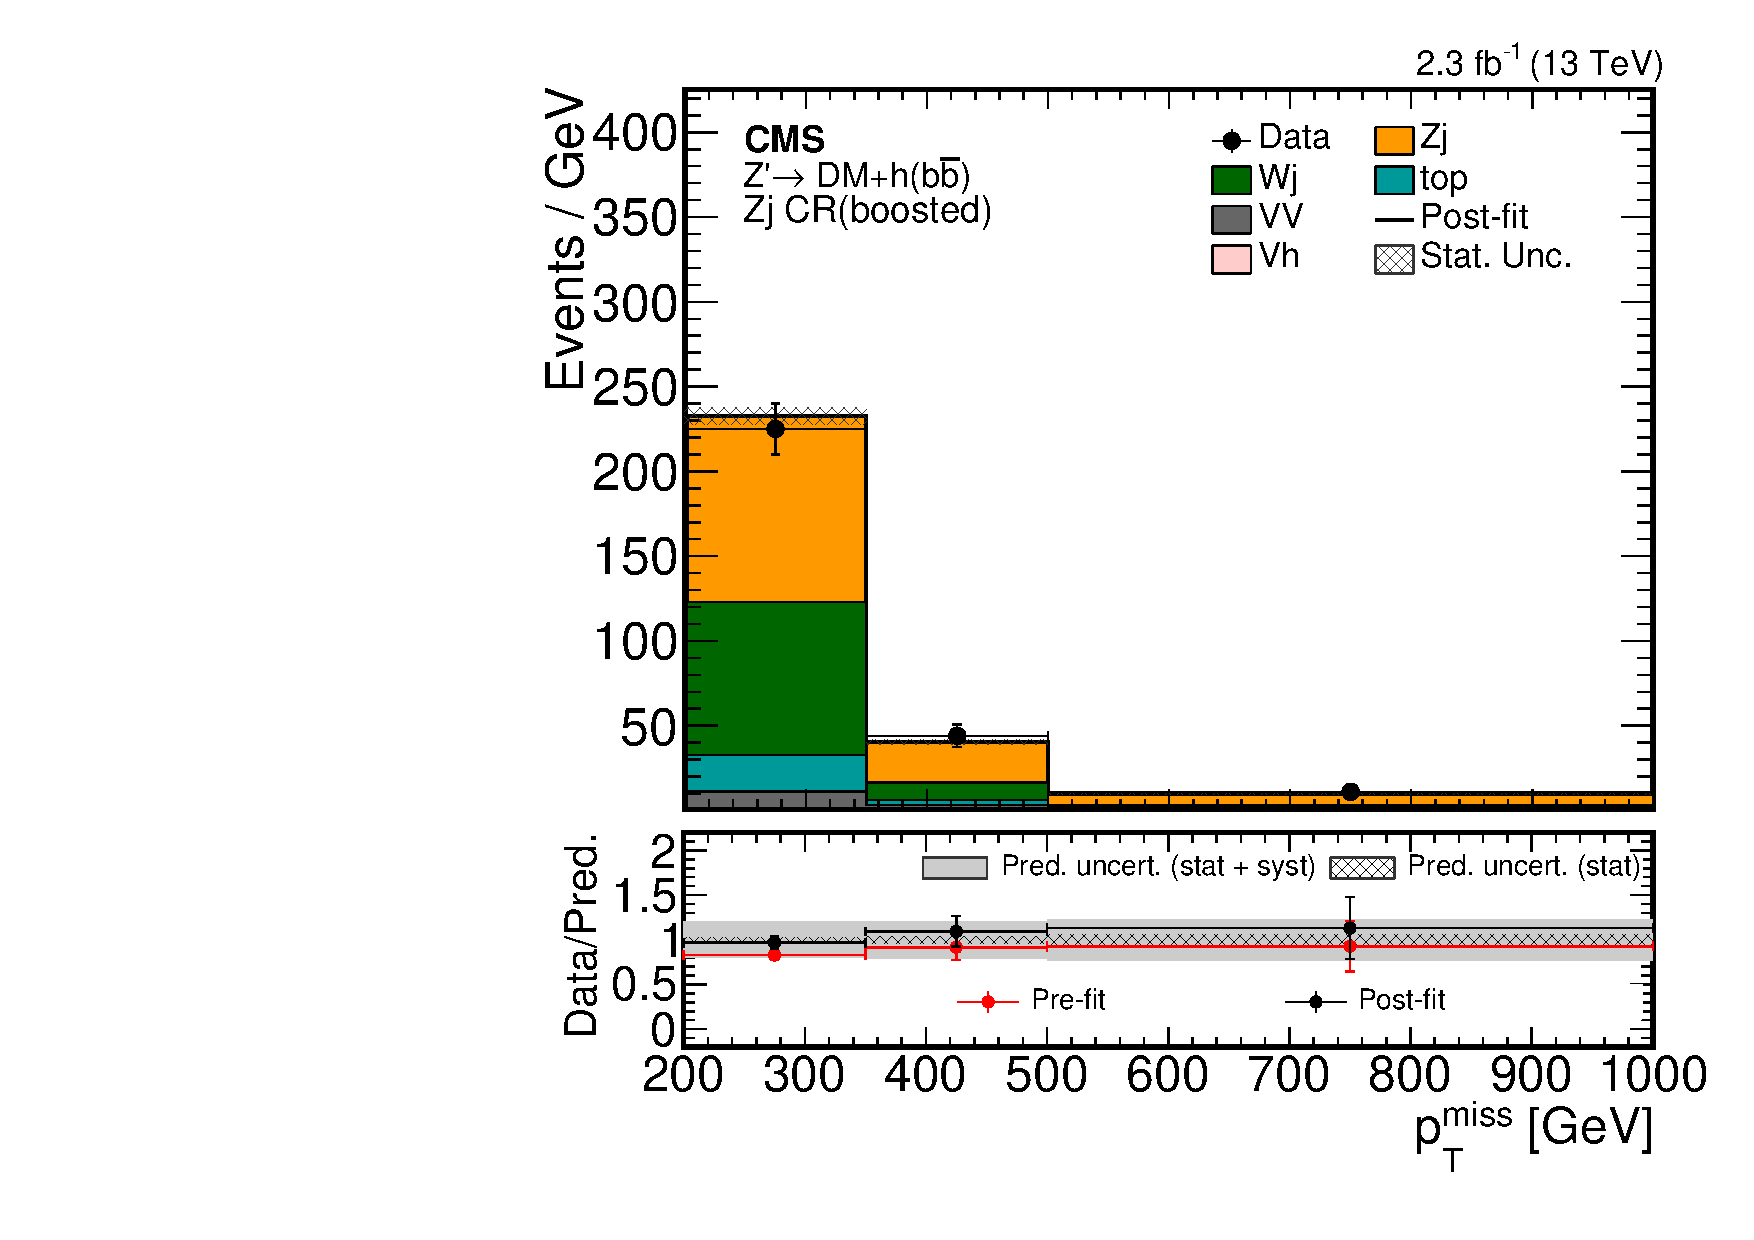
\includegraphics[width=0.49\textwidth]{Figure_005-b.pdf}
\caption{Post-fit distribution of \MET expected from SM backgrounds and observed in data for the single-lepton CR and Z($\rightarrow\nu\overline{\nu}$)+jets CRs for the boosted regime. The bottom panels show the data-to-simulation ratios for pre-fit (red markers) and post-fit (black markers) background predictions with a hatched band corresponding to the uncertainty due to the finite size of simulated samples and a gray band that represents the systematic uncertainty in the post-fit background prediction. The last bin includes all events with $\MET > 500\GeV$.}
\label{fig:controlregionB}
\end{figure}

Figure~\ref{fig:controlregionR} shows the comparison of data and simulation for the main observable, \MET, in the W+jets, top quark, and Z($\rightarrow\nu\overline{\nu}$)+jets  CRs for the resolved regime. 
The comparison between data and simulated samples for the boosted regime is shown in Fig.~\ref{fig:controlregionB} for the single-lepton CR and the Z($\rightarrow\nu\overline{\nu}$) 
mass sideband region. %The last bin in both of these figures contains all events with $\MET > 350$ (500)\GeV for the resolved (boosted) regime. 

Figure~\ref{fig:finalSignalPlots} shows the \MET distributions in three bins in the SR that are used for the final signal extraction. 
These three bins were chosen to optimize the expected limits.
The selected signal and background events are compared to data and fit simultaneously in the SR and CRs in three \MET bins separately 
for the resolved and the boosted regimes. 

The simultaneous fit of SR and background-enhanced CRs is performed correlating the normalization and systematic uncertainties. 
The measured data-to-simulation post-fit scale factors are compatible with unity within the total combined statistical and systematic uncertainty. In particular, for the resolved regime, the scale factors for the backgrounds are 1.23 $\pm$ 0.17 for Z($\rightarrow\nu\overline{\nu}$)+jets,  1.33 $\pm$ 0.19 for W+jets, and 1.13 $\pm$ 0.17 for the top quark 
contributions. 
For the boosted analysis, the scale factors are 0.77 $\pm$ 0.15 for Z($\rightarrow\nu\overline{\nu}$)+jets and 0.95 $\pm$ 0.19 for W+jets and top quark processes. 
Although the background scale factors do not show a common trend between the boosted and resolved analyses, it should be noted that the b-tagging requirement, selected phase space and other parameters are different in the two cases. Thus the two simultaneous fits are essentially independent, allowing the post-fit scale factors to move in either direction from unity.

\begin{figure}[htbp]
\centering
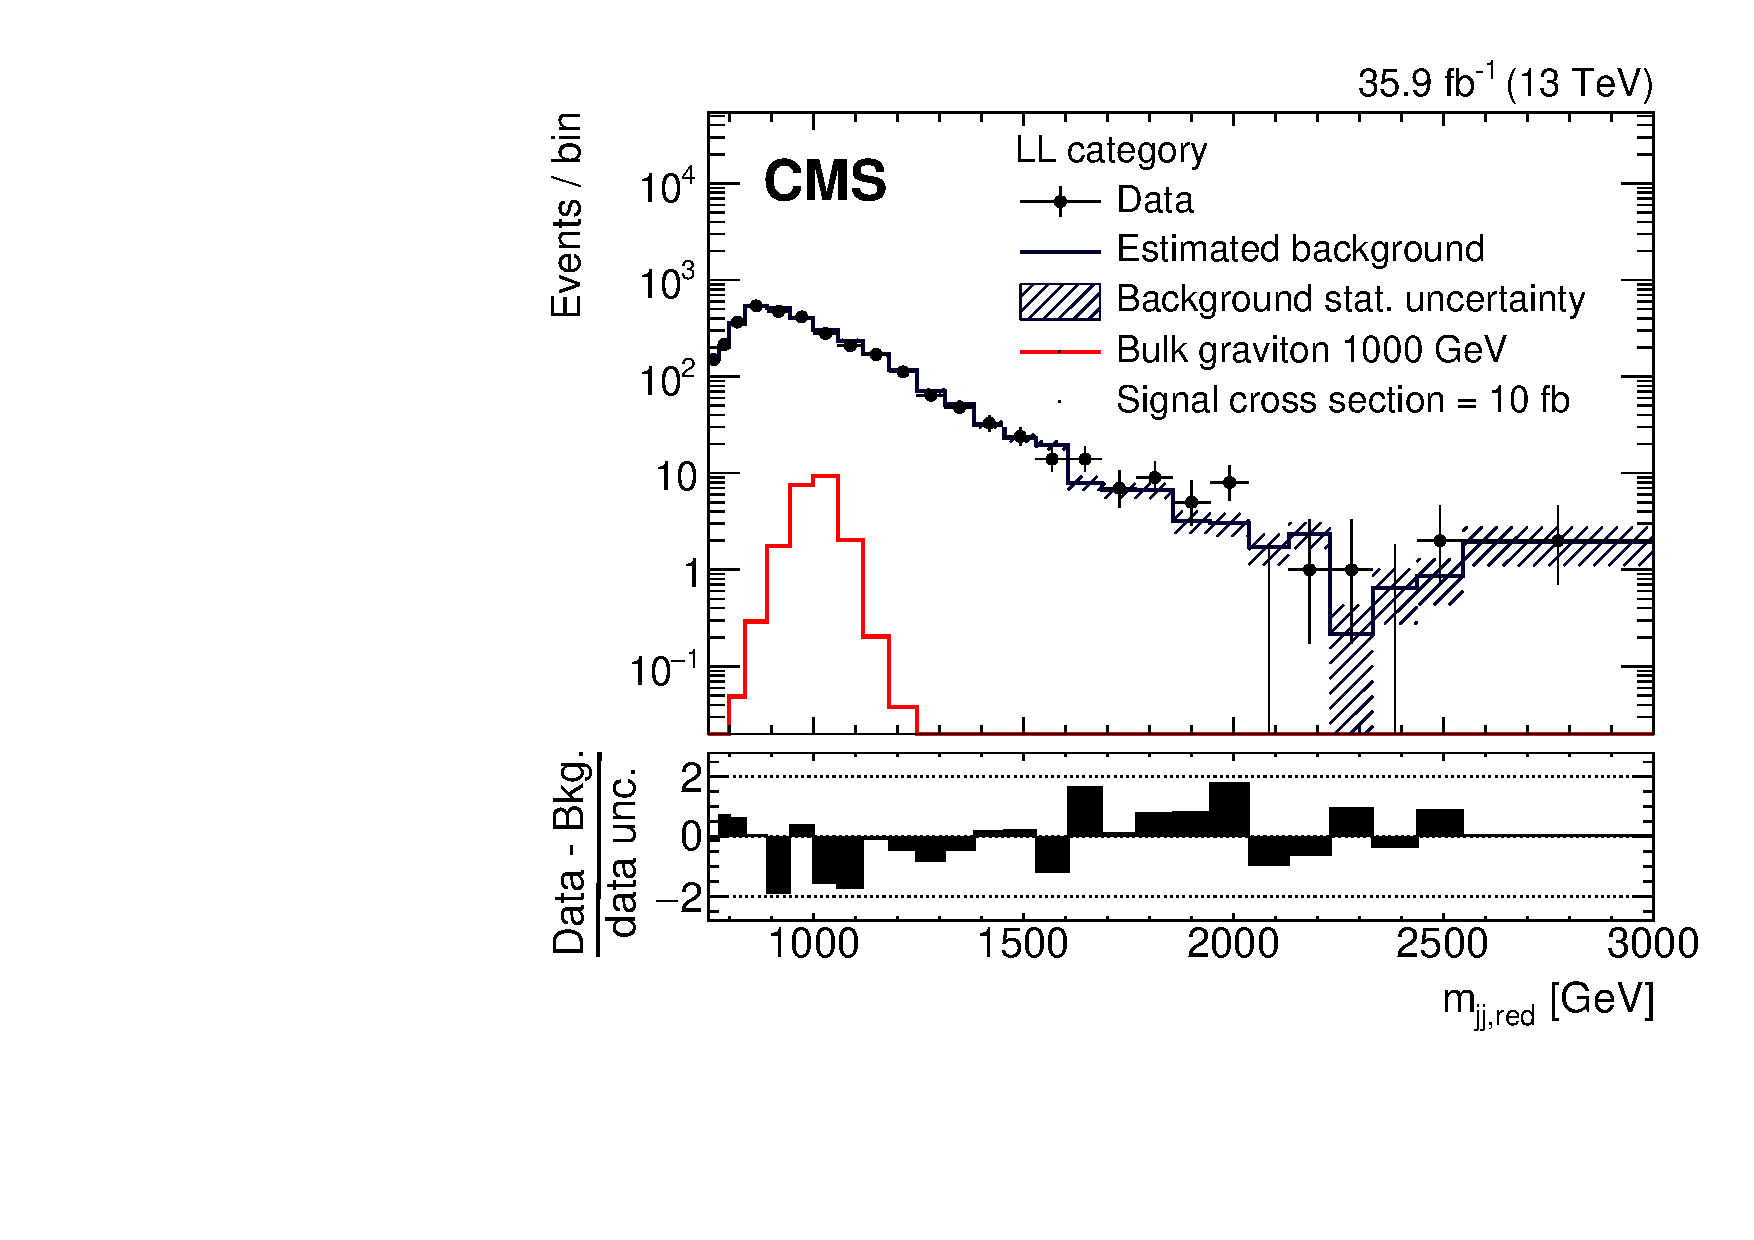
\includegraphics[width=0.49\textwidth]{Figure_006-a.pdf}
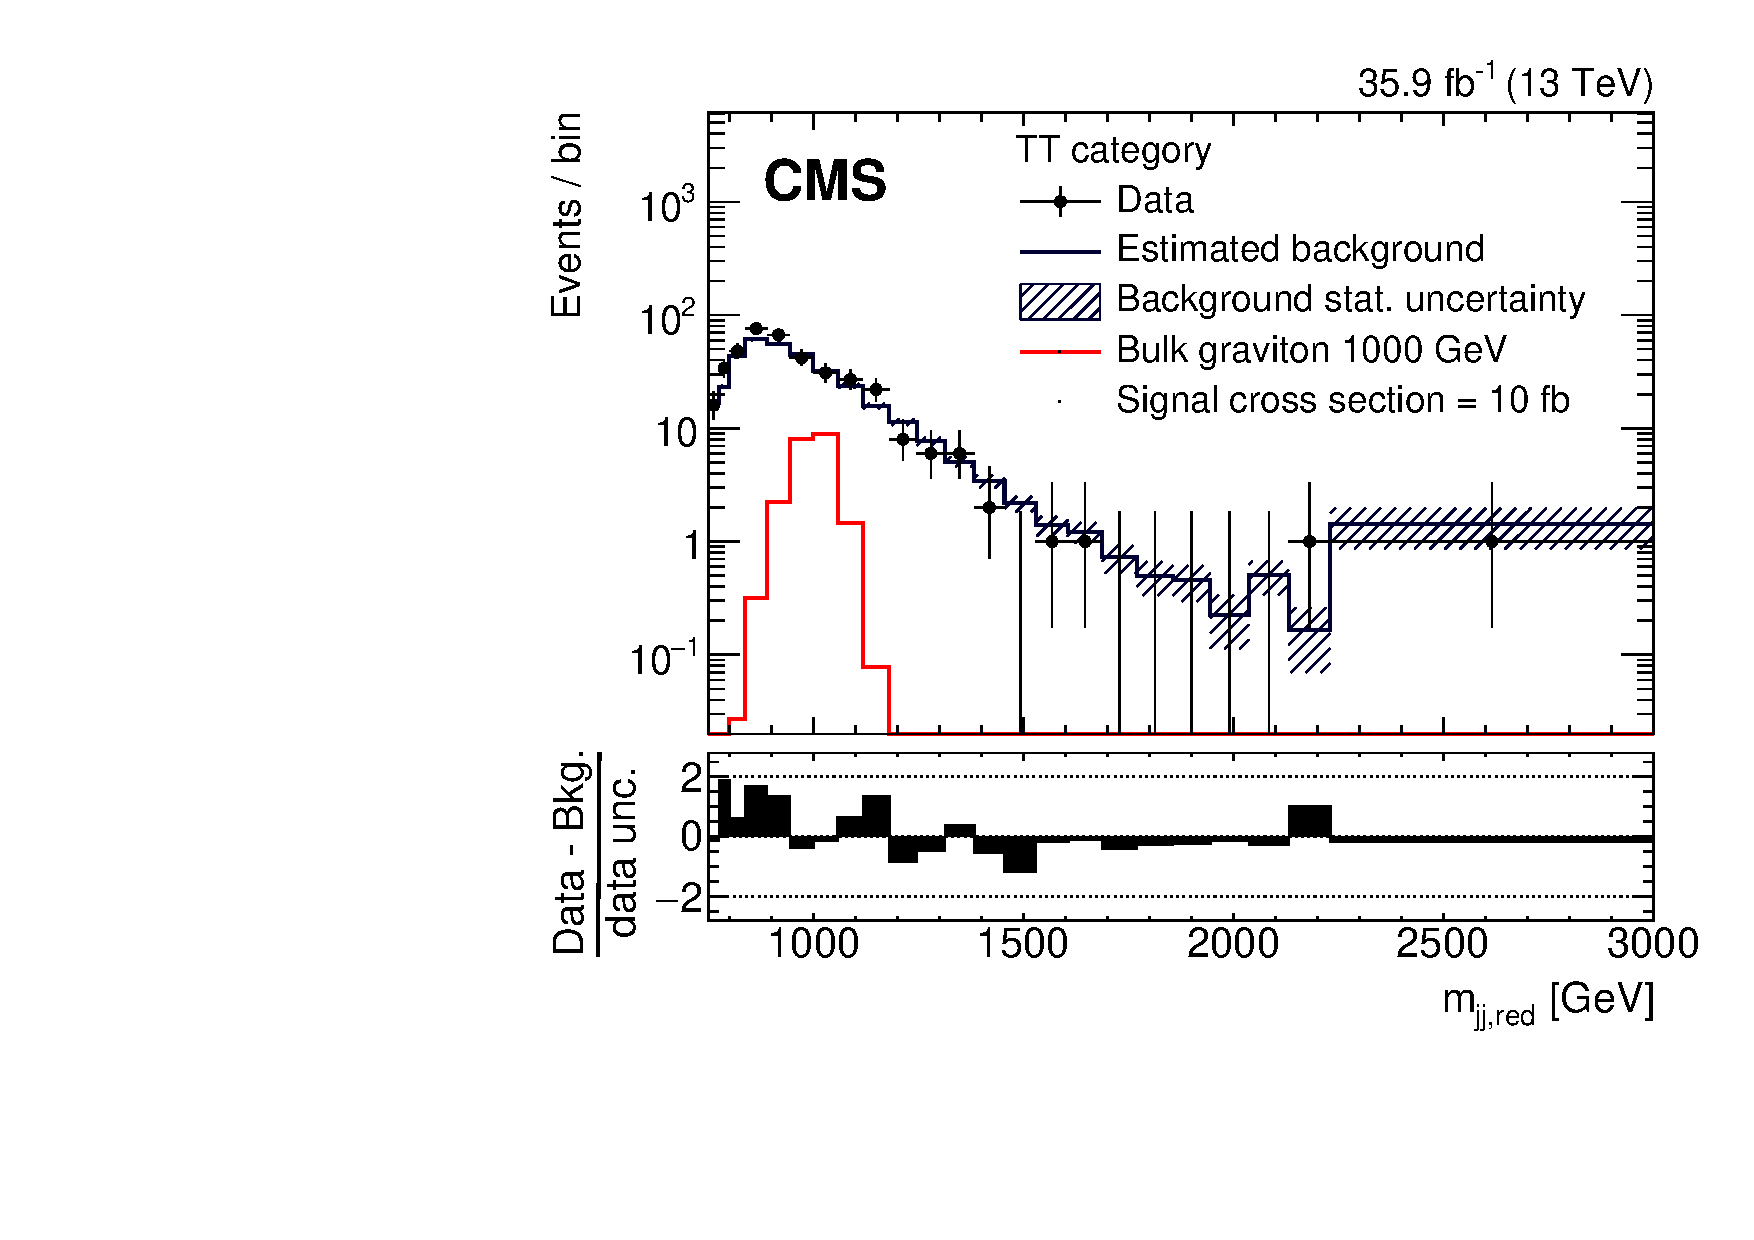
\includegraphics[width=0.49\textwidth]{Figure_006-b.pdf}
\caption{Post-fit distribution of \MET expected from SM backgrounds and observed in data for the resolved (left) and the boosted (right) regimes in the signal region with three different \mzp signal points overlaid. Other parameters for this model are fixed to $m_{\chi} = 100\GeV$ and $\tan{\beta} = g_{\chi} = 1$. The cross sections times branching fractions for the signal models are computed assuming \gzp = 0.8. The bottom panels show the data-to-simulation ratios for pre-fit (red markers) and post-fit (black markers) background predictions with a hatched band corresponding to the uncertainty due to the finite size of simulated samples and a gray band that represents the systematic uncertainty in the post-fit background prediction. The last bin includes all events with $\MET > 350 $ (500)\GeV for the resolved (boosted) regime.}
\label{fig:finalSignalPlots}
\end{figure}



\subsection{Results \label{sec:results}}
For the event selection described in Section~\ref{sec:eventselection}, the predicted signal acceptances multiplied by the efficiencies ($A \epsilon$) are listed in Table~\ref{tab:AcceptanceHGG} for the two decay channels.
 
\begin{table}[bthp]
\centering
\renewcommand{\arraystretch}{1.1}
\topcaption{\label{tab:AcceptanceHGG}
The product of acceptance and efficiency (with statistical uncertainty) for signal in the SR, after full event selection for the \Hbb (upper) and 
the \HGG (lower) decay channels. The systematic uncertainty for \Hbb (\HGG) is approximately 10\% (5\%). For \Hbb, the value shown here is either for the resolved regime or for the boosted regime, depending on which is used for the cross-section limit calculation, as shown in Fig. \ref{fig:limit2d} left. }
\resizebox{\textwidth}{!}{
\begin{tabular}{c|c|c|c|c|c|c}
\begin{tabular}{c} \maz \\ $[\GeV]$ \end{tabular} & 300 & 400 & 500 & 600 & 700 & 800 \\ \hline
\begin{tabular}{c} \mzp \\ $[\GeV]$ \end{tabular} & \multicolumn{6}{c}{\Hbb} \\ \hline 
\x600  & 0.058  $ \pm $ 0.003  & 0.013 $ \pm $ 0.003  &  ---      &  ---  & ---     & ---                                                               \\
\x800  & 0.132  $ \pm $ 0.003  & 0.117 $ \pm $ 0.003  & 0.083 $ \pm $ 0.003  & 0.040 $ \pm $ 0.003  & ---                    & ---                  \\ 
1000 & 0.245  $ \pm $ 0.004  & 0.218 $ \pm $ 0.003  & 0.167 $ \pm $ 0.002  & 0.123 $ \pm $ 0.003  & 0.181 $ \pm $ 0.003  & 0.066$ \pm $ 0.003 \\
1200 & 0.282  $ \pm $ 0.003  & 0.272 $ \pm $ 0.004  & 0.262 $ \pm $ 0.003  & 0.238 $ \pm $ 0.004  & 0.195 $ \pm $ 0.003  & 0.126$ \pm $ 0.003 \\
1400 & 0.286  $ \pm $ 0.003  & 0.287 $ \pm $ 0.003  & 0.283 $ \pm $ 0.003  & 0.279 $ \pm $ 0.003  & 0.285 $ \pm $ 0.003  & 0.249$ \pm $ 0.003 \\
1700 & 0.280  $ \pm $ 0.003  & 0.284 $ \pm $ 0.003  & 0.283 $ \pm $ 0.003  & 0.284 $ \pm $ 0.003  & 0.285 $ \pm $ 0.004  & 0.284$ \pm $ 0.003 \\
2000 & 0.269  $ \pm $ 0.005  & 0.271 $ \pm $ 0.003  & 0.275 $ \pm $ 0.003  & 0.273 $ \pm $ 0.003  & 0.276 $ \pm $ 0.003  & 0.279$ \pm $ 0.004 \\
2500 & 0.248  $ \pm $ 0.003  & 0.246 $ \pm $ 0.003  & 0.250 $ \pm $ 0.004  & 0.251 $ \pm $ 0.003  & 0.255 $ \pm $ 0.003  & 0.256$ \pm $ 0.003 \\
\hline 
\begin{tabular}{c} \mzp \\ $[\GeV]$ \end{tabular}  & \multicolumn{6}{c}{\HGG} \\ 
\hline
600     & 0.317 $ \pm $ 0.004 & 0.212 $ \pm $ 0.003 & --- & --- & --- & ---                                                                 \\
800     & 0.399 $ \pm $ 0.004 & 0.386 $ \pm $ 0.003 & 0.348 $ \pm $ 0.003 &  0.280 $\pm$ 0.003  & --- & ---                                 \\
1000 	& 0.444 $ \pm $ 0.004 & 0.437 $ \pm $ 0.003 & 0.422 $ \pm $ 0.003 & 0.402 $ \pm $ 0.003 & 0.373 $ \pm $ 0.003 & 0.330 $ \pm $ 0.003 \\
1200 	& 0.474 $ \pm $ 0.004 & 0.468 $ \pm $ 0.003 & 0.461 $ \pm $ 0.003 & 0.454 $\pm$ 0.003  & 0.438 $ \pm $ 0.003 & 0.417 $ \pm $ 0.003  \\
1400 	& 0.492 $ \pm $ 0.004 & 0.493 $ \pm $ 0.003 & 0.485 $ \pm $ 0.003 & 0.481 $ \pm $ 0.003 & 0.472 $ \pm $ 0.003 & 0.465 $ \pm $ 0.003 \\
1700 	& 0.493 $ \pm $ 0.004 & 0.499 $ \pm $ 0.003 & 0.504 $ \pm $ 0.003 & 0.503 $ \pm $ 0.003 & 0.499 $ \pm $ 0.003 & 0.498 $ \pm $ 0.003 \\
2000 	& 0.351 $ \pm $ 0.004 & 0.373 $ \pm $ 0.003 & 0.394 $ \pm $ 0.003 & 0.421 $ \pm $ 0.003 & 0.453 $ \pm $ 0.003 & 0.488 $ \pm $ 0.003 \\
2500 	& 0.213 $ \pm $ 0.004 &  0.217 $\pm$ 0.003  & 0.227 $ \pm $ 0.003 & 0.236 $ \pm $ 0.003 & 0.254 $ \pm $ 0.003 & 0.268 $ \pm $ 0.003 \\
\end{tabular}
}
\end{table}

\begin{table}[http]
\topcaption{Post-fit background event yields and observed numbers of events in data for 2.3\fbinv in both the resolved and the boosted regimes for the \Hbb analysis. The expected numbers of signal events for $m_{\mathrm{A}} = 300\GeV$, scaled to the nominal cross section with $\gzp = 0.8$, are also reported. The statistical and systematic uncertainties are shown separately in that order.
%. reported. The errors shown in the table include both statistical and systematic uncertainty.
\label{tab:eventYieldTable} }
\small
\begin{center}
\begin{tabular}{c|cc}
{\Hbb analysis}& \multicolumn{2}{c}{Number of events (in 2.3\fbinv)}\\
\hline
Process                           & Resolved  & Boosted \\
\hline
% stats and systematics summed up 
%$Z(\rightarrow \nu\overline{\nu})$+jets   & 29.6 $\pm$ 4.9\x   &     19.3 $\pm$ 2.0\x  \\
%top quark                         & 7.3 $\pm$ 2.1   &     8.2 $\pm$ 2.3  \\
%W+jets                       & 9.1 $\pm$ 2.2   &     10.7 $\pm$ 2.6\x  \\
%Diboson                      & 2.7 $\pm$ 0.7   &     1.5 $\pm$ 0.5  \\
%Vh                           & 2.0 $\pm$ 0.2   &     0.8 $\pm$ 0.2   \\
%Multijet                          & 0.010 $\pm$ 0.002 & 0.02 $\pm$ 0.01 \\
%
$Z(\rightarrow \nu\overline{\nu})$+jets   & 29.6 $\pm$ 2.7 $\pm$ 4.1\x   &     19.3 $\pm$ 0.8  $\pm$ 1.8\x  \\
top quark                                 & 7.3 $\pm$ 1.8 $\pm$ 1.0      &     8.2 $\pm$ 1.7   $\pm$ 1.6                  \\
W+jets                                    & 9.1 $\pm$ 1.6 $\pm$ 1.5      &     10.7 $\pm$ 1.6  $\pm$ 2.0\x  \\
Diboson                                   & 2.7 $\pm$ 0.5 $\pm$ 0.5      &     1.5 $\pm$ 0.3   $\pm$ 0.4                 \\
Vh                                        & 2.0 $\pm$ 0.02 $\pm$ 0.2     &     0.8 $\pm$ 0.05  $\pm$ 0.2                  \\
Multijet                                  & 0.01 $\pm$ 0.01 $\pm$ 0.20  &     0.02 $\pm$ 0.01 $\pm$ 0.01              \\
\hline
Total background             &50.7 $\pm$ 2.9 $\pm$   4.6 \x  &     40.5 $\pm$ 2.4 $\pm$ 3.1\x   \\
\hline
Data                       & 44        & 38     \\
\multicolumn{3}{c}{}        \\ [-1.0ex]
 \mzp $[\GeV]$           &      \multicolumn{2}{c}{}        \\
\hline
\x600                        &  29.0 $\pm$ 0.4 $\pm$ 3.5\x     & --- \\
\x800                        &  40.4 $\pm$ 0.5 $\pm$ 3.8\x     & ---   \\
1000                       &  23.3 $\pm$ 0.3 $\pm$  2.5\x & ---  \\
1200                       & ---    & 23.6 $\pm$ 0.4  $\pm$  2.4\x  \\
1400                       & ---    & 13.1 $\pm$ 0.3  $\pm$   1.4\x  \\
1700                       & ---    & 5.6 $\pm$  0.2  $\pm$   0.7   \\
2000                       & ---    & 2.3 $\pm$  0.1   $\pm$  0.3   \\
2500                       & ---    & 0.24 $\pm$ 0.01  $\pm$  0.03  \\
\end{tabular}
\end{center}
\end{table}

Table \ref{tab:eventYieldTable} shows, for the \Hbb channel, the 
SR post-fit yields for each background and signal mass point along with the sum of the statistical and systematic uncertainties for the resolved and boosted regimes. The total background uncertainty is approximately 10\% and mainly driven by the systematic uncertainty. 



Since no excess of events has been observed over the SM background expectation in the signal region, the results of this search are interpreted in terms of an upper limit on the production cross section of DM candidates in association with a Higgs boson via $\PZpr \rightarrow \Az \Ph \rightarrow \chi \overline{\chi} \, \PAQb\PQb(\gamma\gamma)$. 
The upper limits are computed at 95\% confidence level (CL) using a modified frequentist method (CL$_s$) \cite{yellowReport, bib:CLS1, bib:CLS2} computed with an asymptotic approximation \cite{bib:CLS3}. 
A profile likelihood ratio is used as the test statistic in which systematic uncertainties are modeled as nuisance parameters.
These limits are obtained as a function of \mzp and \maz for both Higgs boson decay channels and for the combination of the two.
The two decay channels are combined using the branching ratios predicted by the SM.
In the combination of the two analyses, all signal and \MET-related systematic uncertainties as well as the systematic uncertainty in the integrated luminosity 
are assumed to be fully correlated.

Figure~\ref{fig:limitsexpected}  (left) shows the 95\% CL expected and observed limits on the dark matter production cross section for \Hbb and \HGG for \maz = 300\GeV. These results, obtained with $m_{\chi}= 100\GeV$, can be considered valid for any dark matter mass below 100\GeV since the branching fraction for decays of \Az to DM particles, ${\cal B}(\Az\rightarrow\chi\overline{\chi})$, decreases as $m_{\chi}$ increases.
As shown in Figure~\ref{fig:limitsexpected}, for the phase space parameters considered for this model ($g_{\chi}$ and $\tan{\beta}$ equal to unity), results of the combined analysis are mainly driven by the \Hbb channel. The combination with the \HGG channel provides a 2-4\% improvement in terms of constraints on the model for the low \PZpr mass values. Future iterations of this search will explore additional phase space regions of the \cPZpr-2HDM model, i.e. larger values of $\tan{\beta}$, where the \HGG channel becomes more sensitive than \Hbb~\cite{2HDM}.

Figures~\ref{fig:limitsexpected} (right) and~\ref{fig:limit2d} show the 95\% CL  expected and observed upper limits on the signal strength. 
For \maz = 300\GeV, the \PZpr mass range from 600 to 1780\GeV is expected to be excluded with a 95\% CL when the signal model 
cross section is calculated using \gzp = 0.8, while the 
observed data, for \maz = 300\GeV exclude the \zp mass range from 600 to 1860\GeV. 
When the signal model cross section is calculated using the constrained \gzp, the expected exclusion range is 830 to 1890\GeV, 
and the observed exclusion range is 770 to 2040\GeV. 
Figure~\ref{fig:limit2d} shows the expected and observed upper limits on the signal strength for the \Hbb and \HGG decay channels. 
Figure~\ref{fig:limit2dcombo} shows the upper limits on the signal strength combining the results from both the \Hbb and \HGG decay channels. 

\begin{figure}[htbp]
\centering
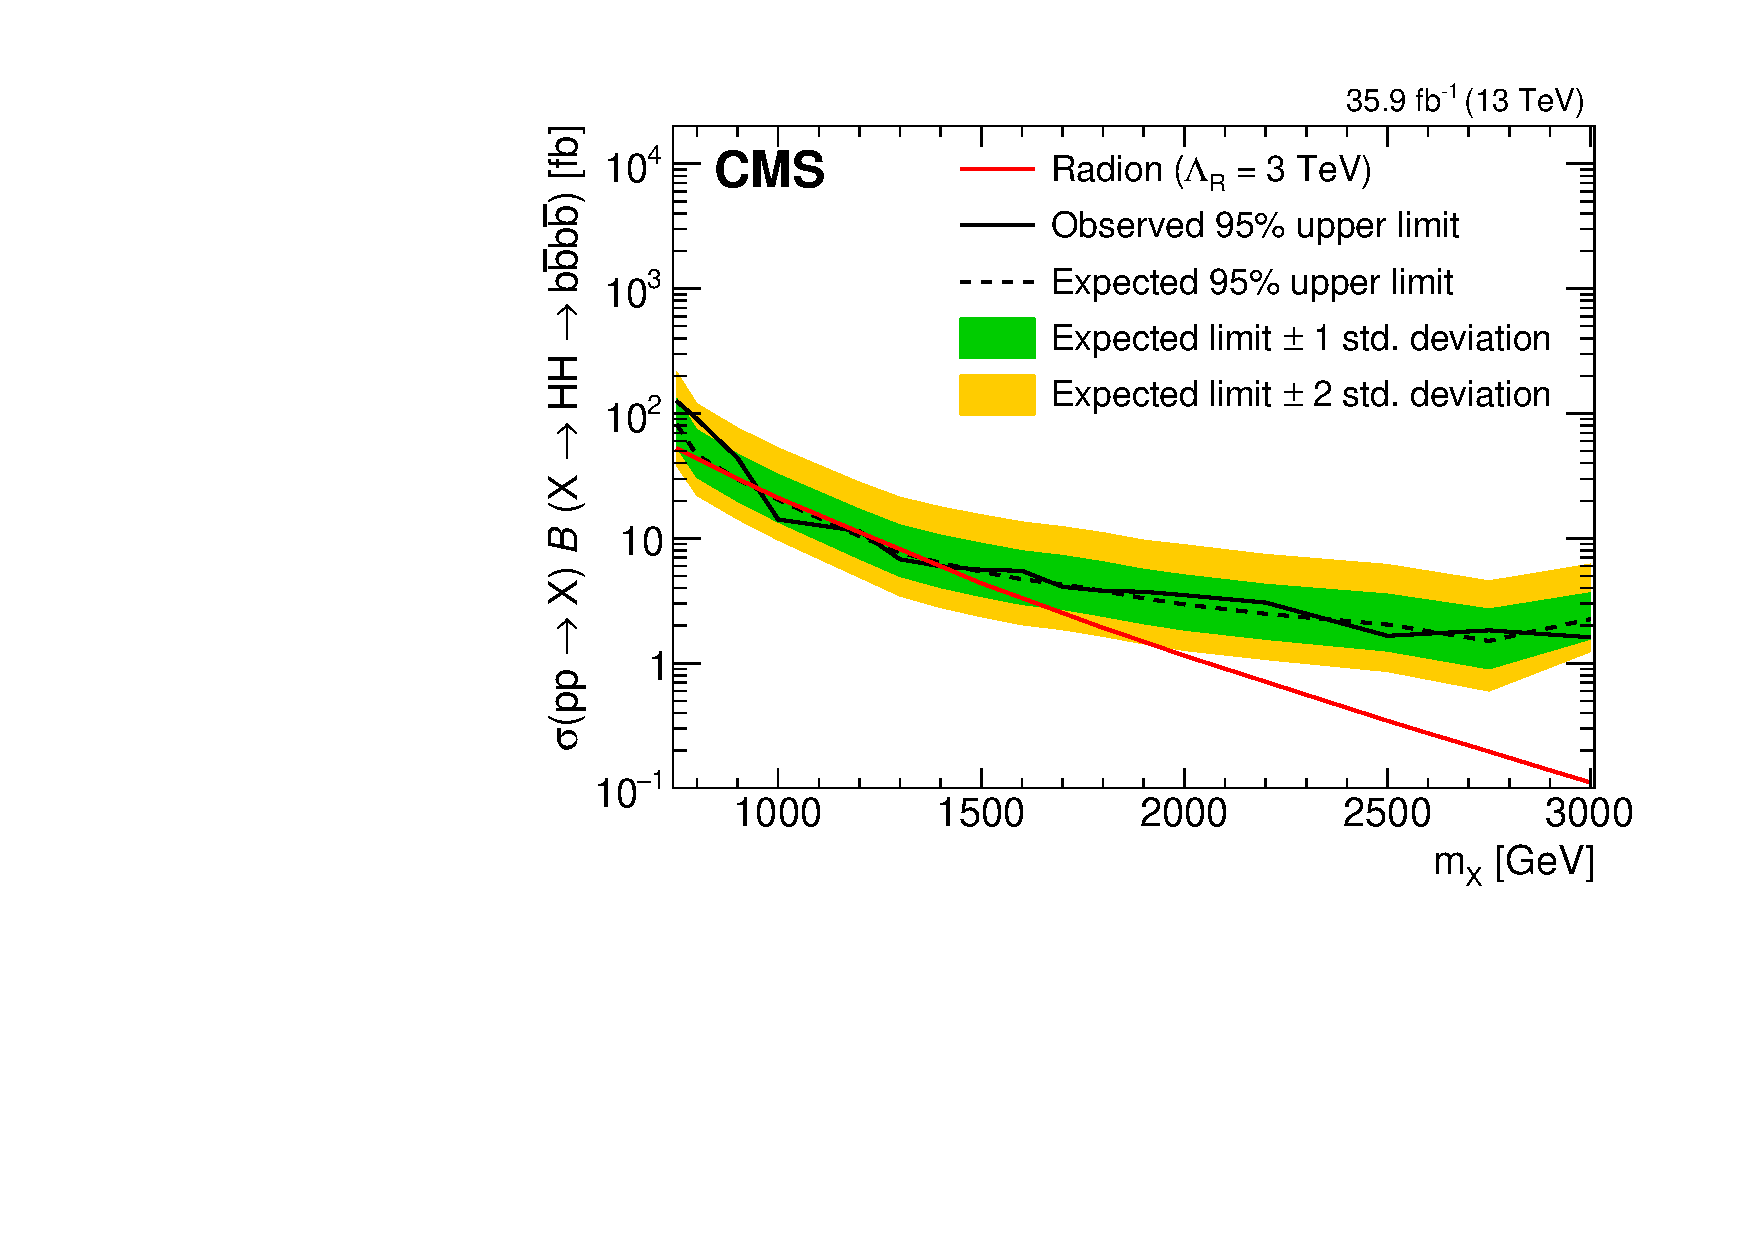
\includegraphics[width=0.45\textwidth]{Figure_009-a.pdf}
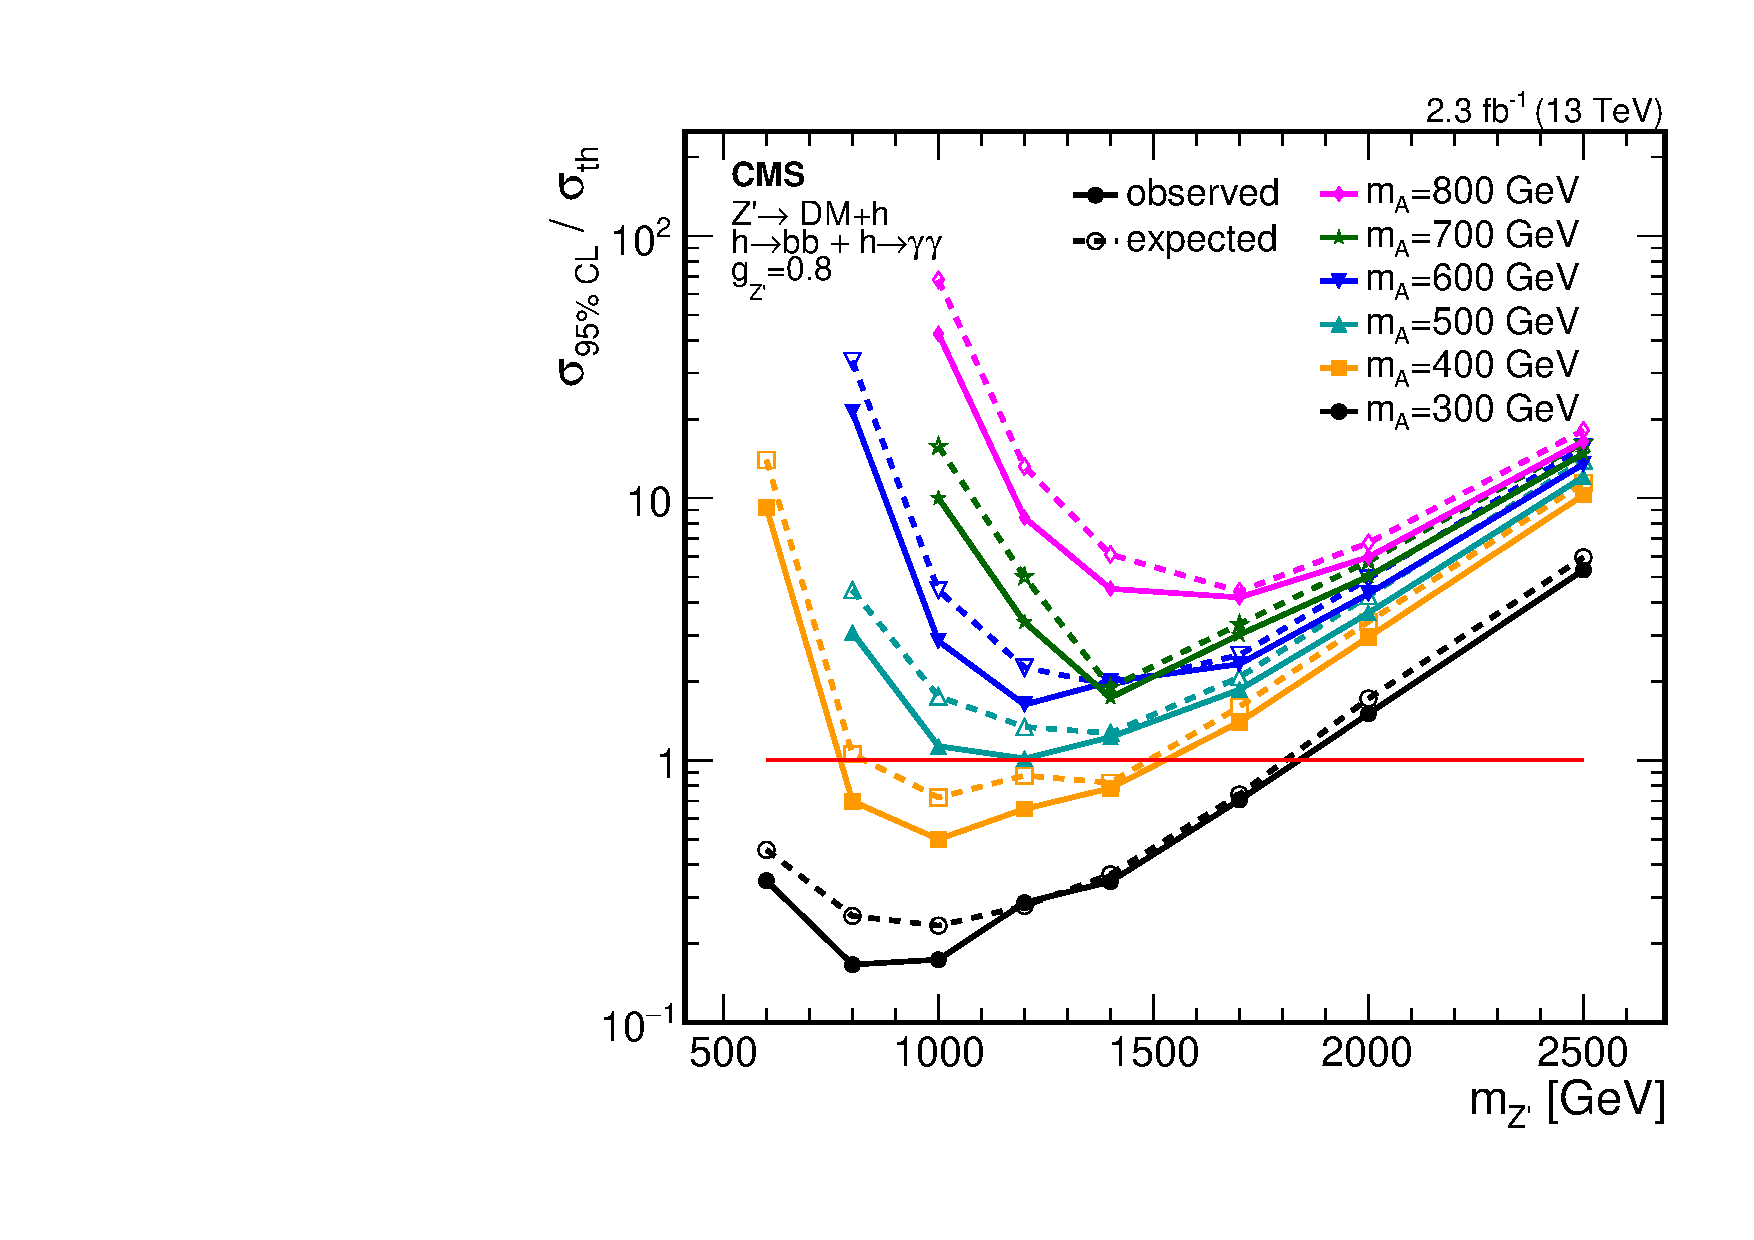
\includegraphics[width=0.45\textwidth]{Figure_009-b.pdf}
\caption{Left: The expected and observed 95\% CL limits 
on dark matter production cross sections for \Hbb and \HGG for \maz = 300\GeV. The exclusion region is shown for two 
\gzp values. The dark green and light yellow  bands show the 68\% and 95\% uncertainties on the expected limit.
Right: The expected and observed 95\% CL limits on the signal strength for \maz = 300--800\GeV are shown.
Other parameters for this model are fixed to $m_{\chi} = 100\GeV$ and $\tan{\beta} = g_{\chi} = 1$. 
The theoretical cross section ($\sigma_{\mathrm{th}}$) used for the right-hand plot is calculated using \gzp = 0.8.}
\label{fig:limitsexpected}
\end{figure}

\begin{figure}[htbp]
\centering
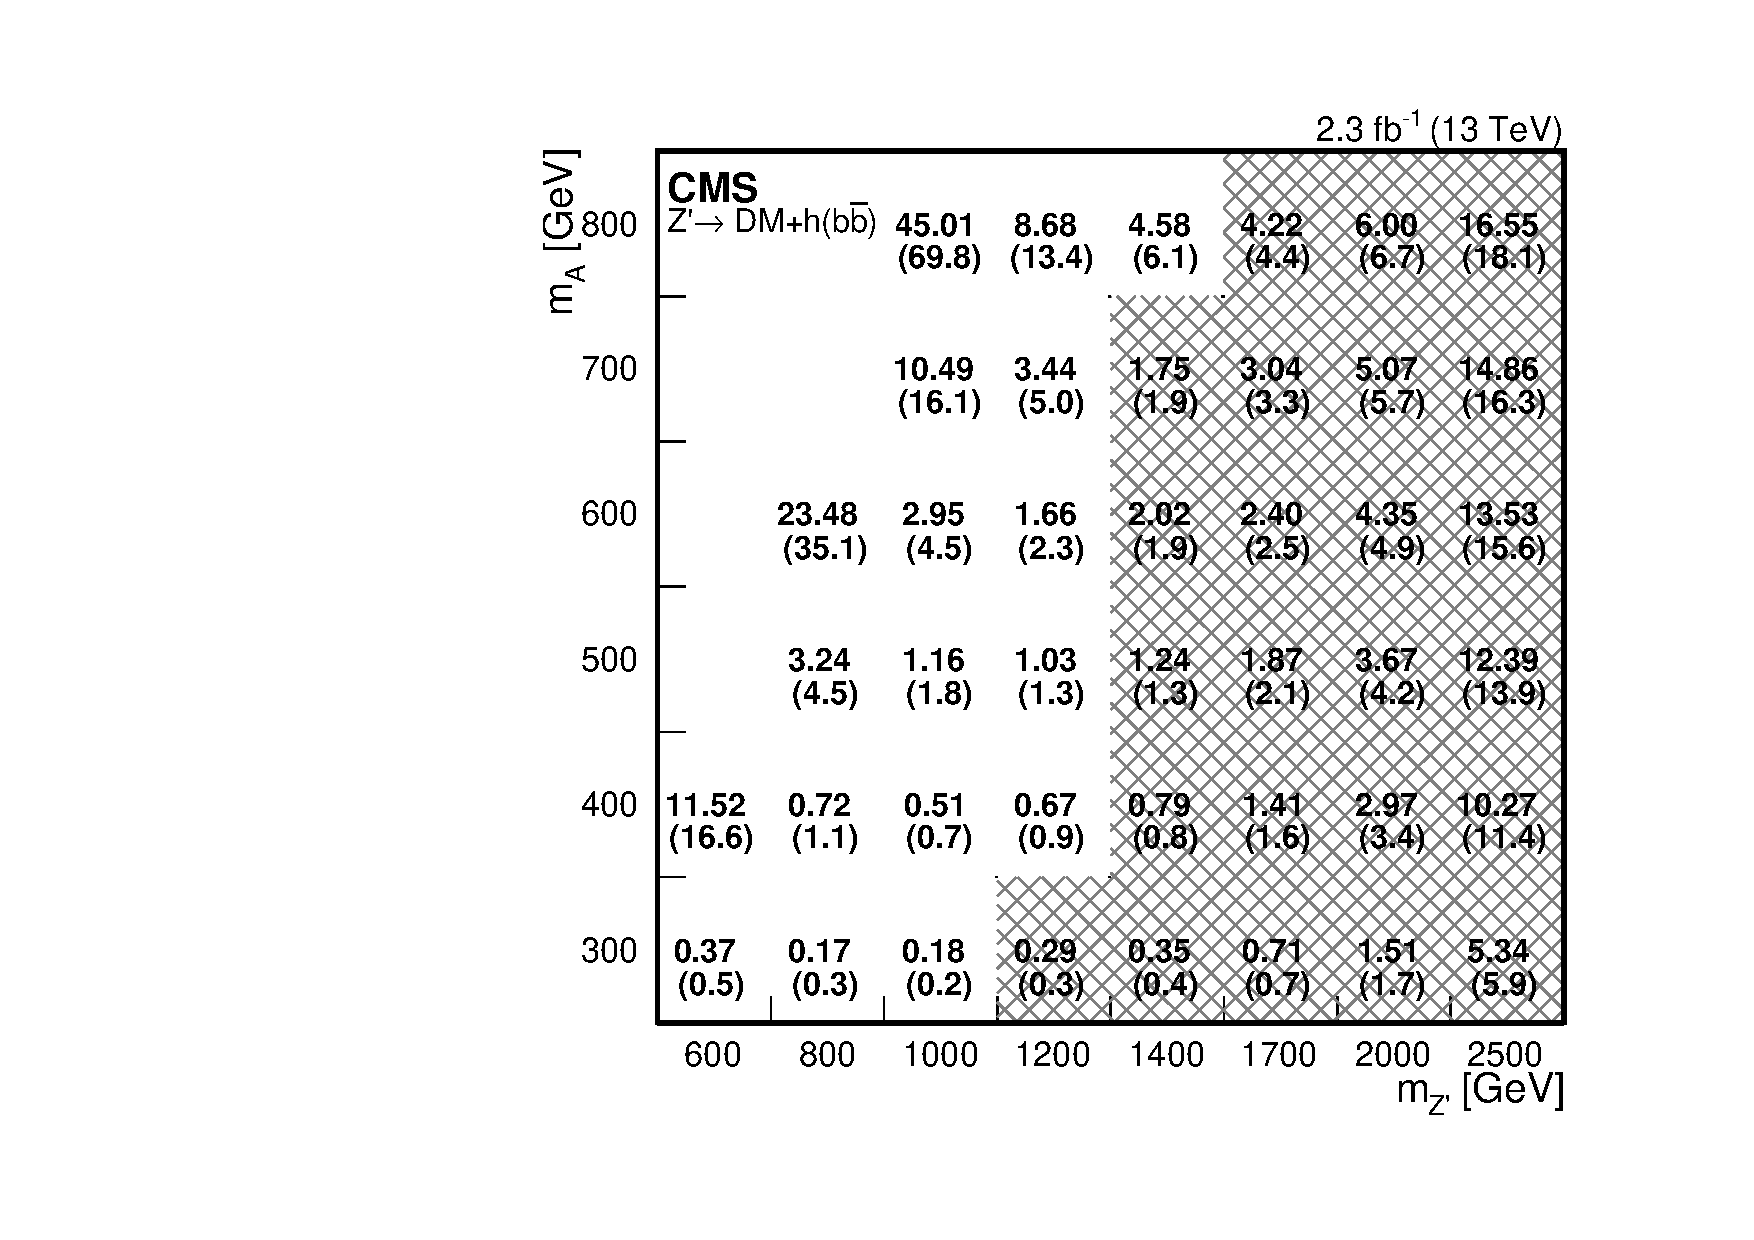
\includegraphics[width=0.45\textwidth]{Figure_010-a.pdf}
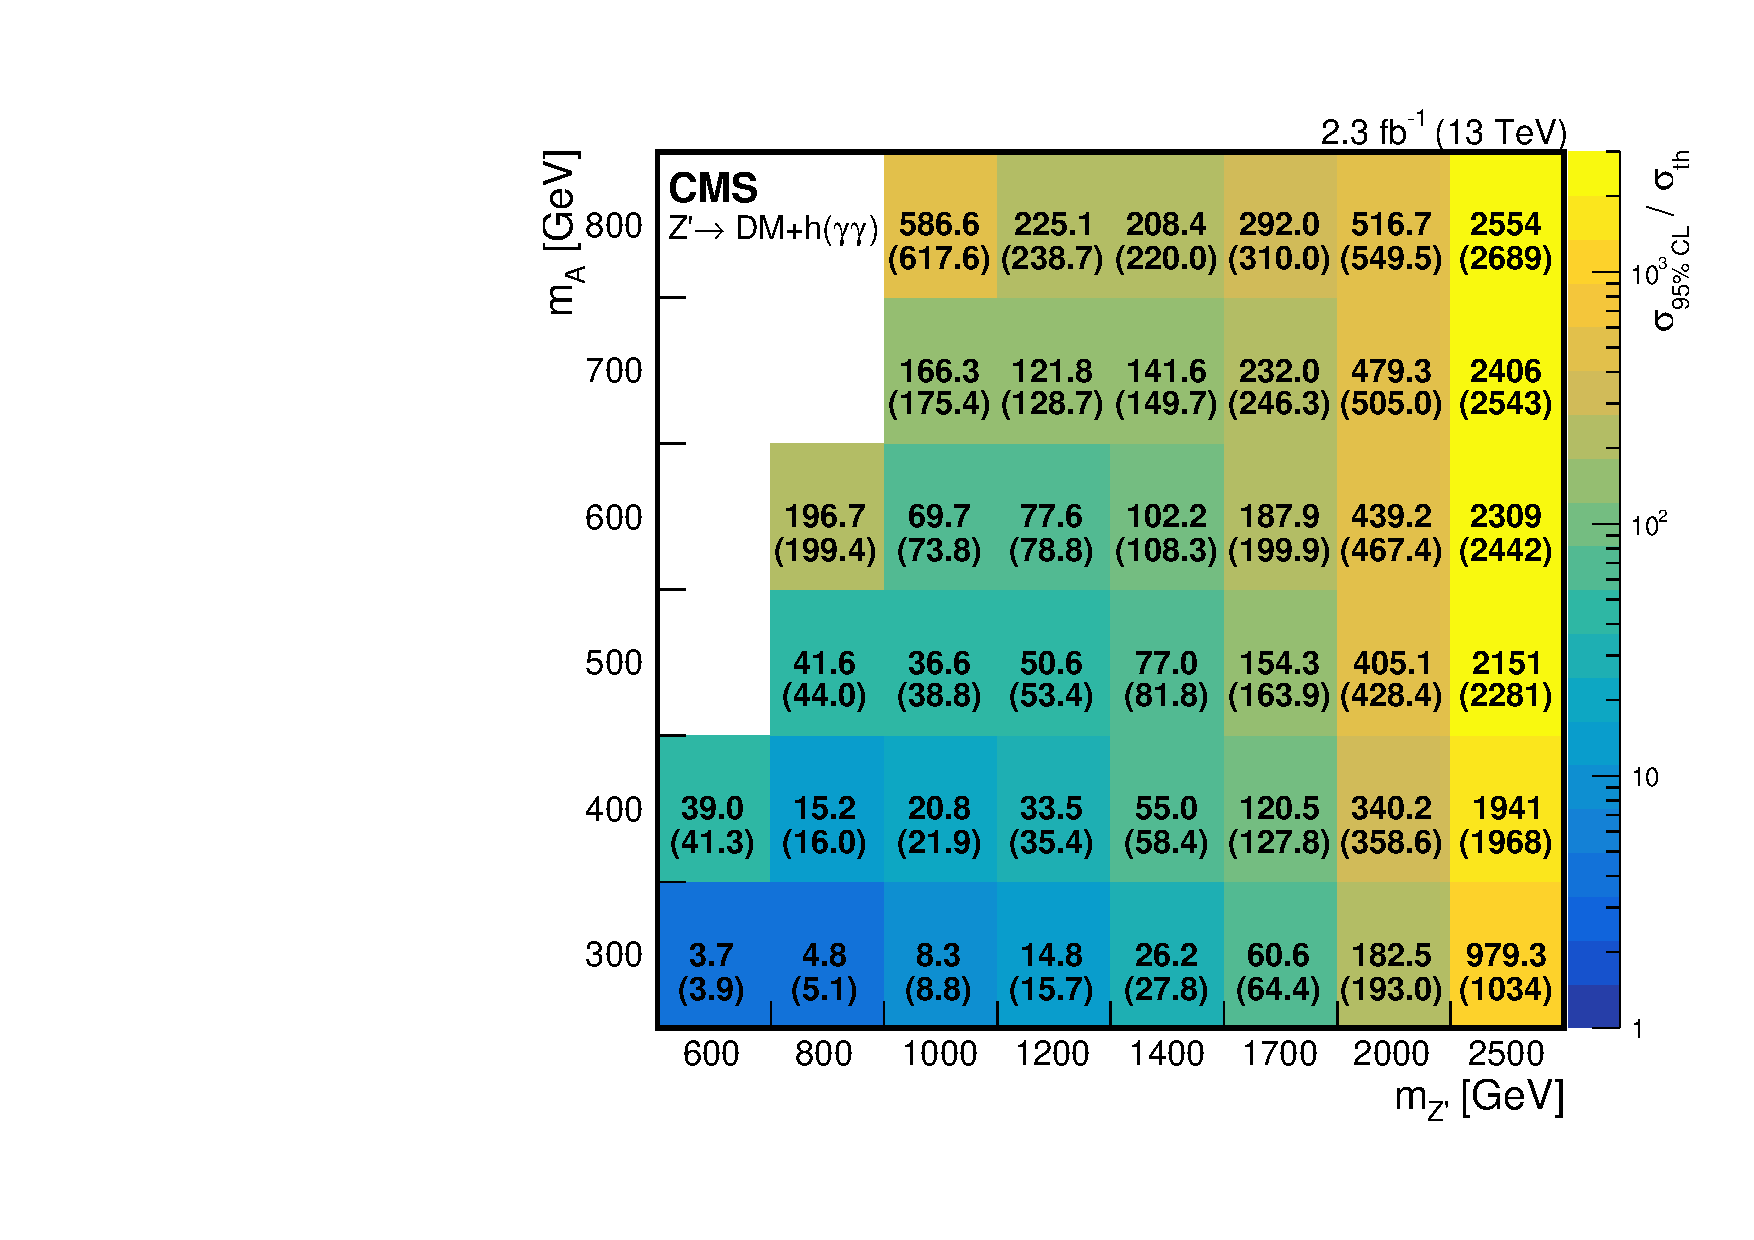
\includegraphics[width=0.45\textwidth]{Figure_010-b.pdf}
\caption{The observed (expected) 95\% CL limits on the signal strength (as in Fig.~\ref{fig:limitsexpected} right), separately for the \Hbb (left) and \HGG (right) decay channels, and for \maz = 300--800\GeV and \mzp = 600--2500\GeV. Other parameters for this model are fixed to $m_{\chi} = 100\GeV$ and $\tan{\beta} = g_{\chi} = 1$. The theoretical cross sections times branching fractions are calculated using $g_{\zp} = 0.8$. For \Hbb, the results for the resolved analysis are shown over a white background, whereas the boosted analysis results are shown over a hatched background. }
\label{fig:limit2d}
\end{figure}

\begin{figure}[htbp]
\centering
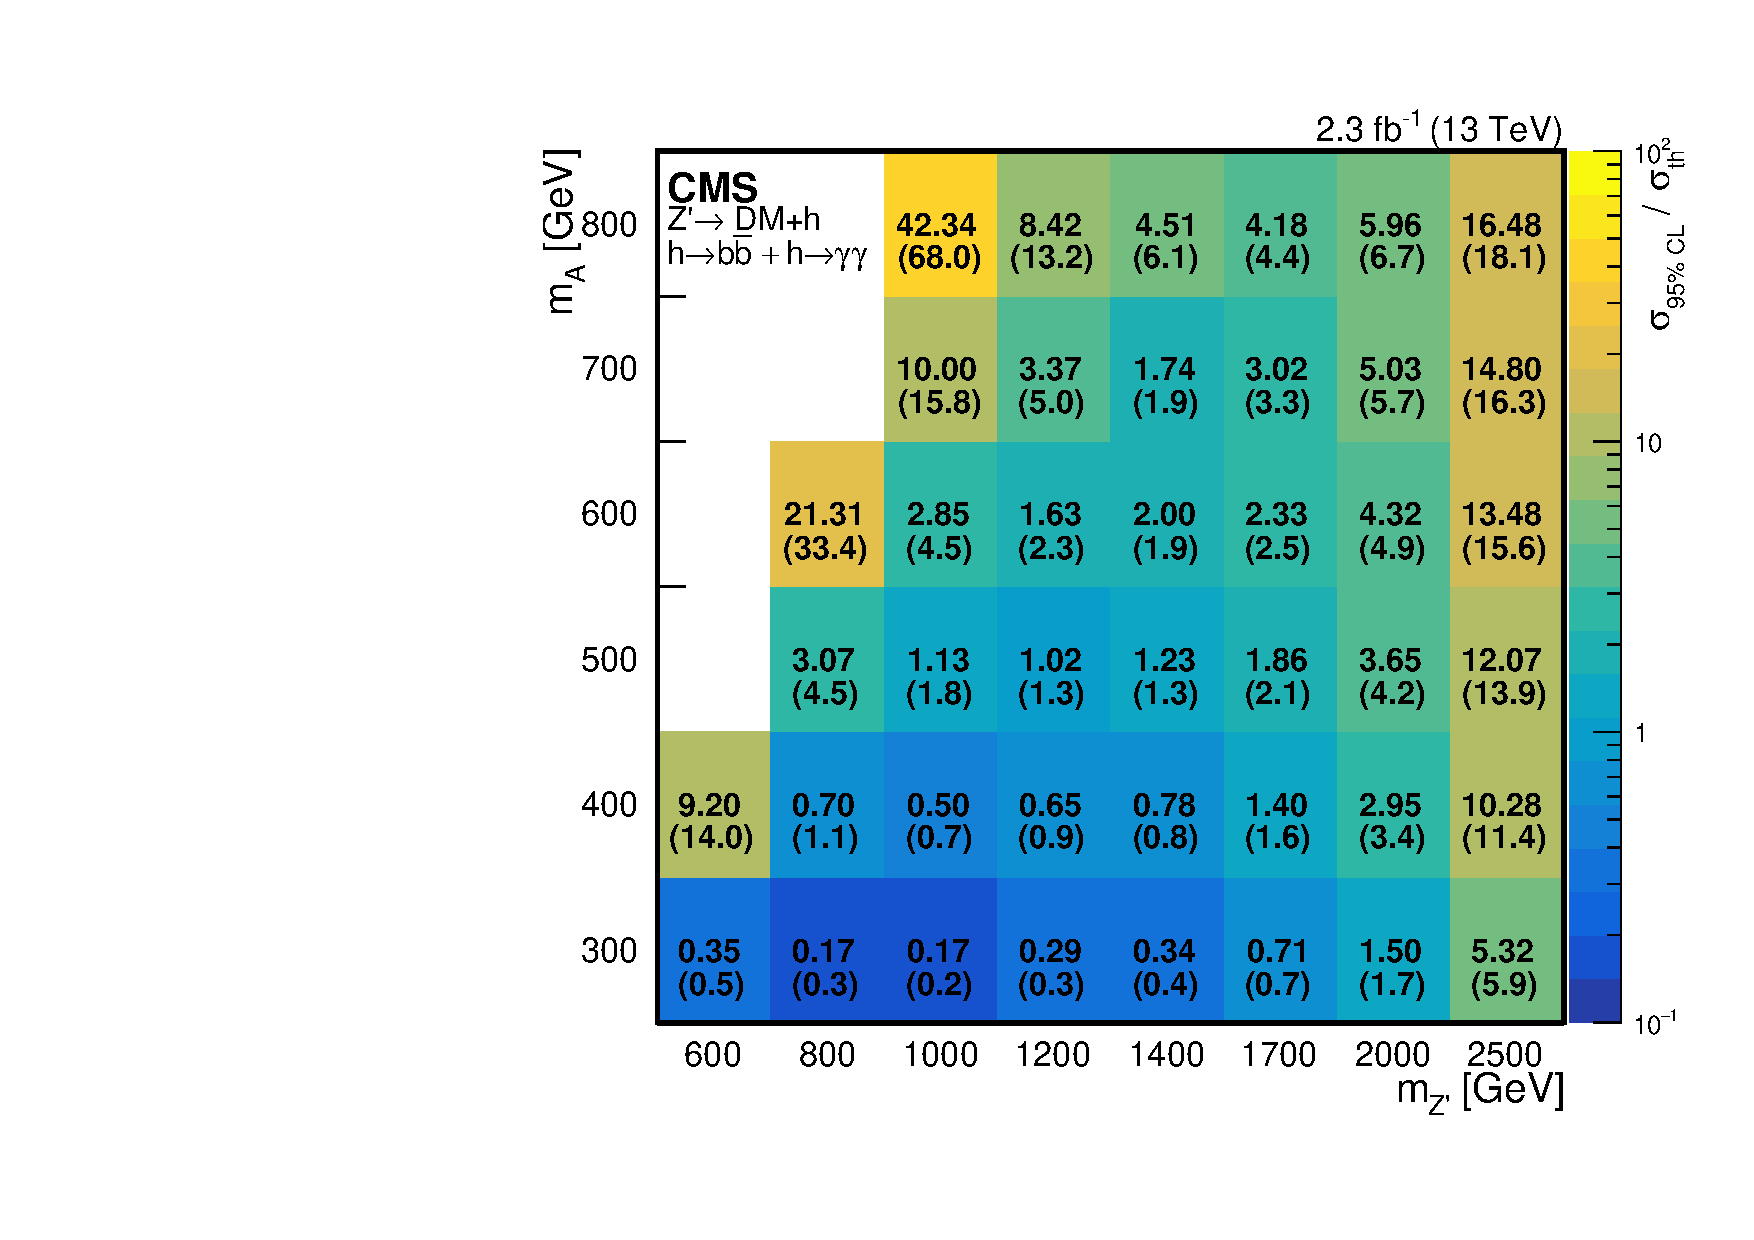
\includegraphics[width=0.45\textwidth]{Figure_011.pdf}
\caption{The observed (expected) 95\% CL limits on the signal strength (as in Fig.~\ref{fig:limitsexpected} right) for the combination of \HGG and \Hbb decay channels, and for \maz = 300--800\GeV and \mzp = 600--2500\GeV. Other parameters for this model are fixed to $m_{\chi} = 100$ \GeV and $\tan{\beta} = g_{\chi} = 1$. The theoretical cross sections times branching fractions are calculated using $g_{\zp} = 0.8$.}
\label{fig:limit2dcombo}
\end{figure}


%%%%%%%%%%%%%%%%%%%%%%%%%%%%%%%%%%%%%%%%%%%%%%%%%%%%%%%%%%%%%%%%%%%%%%%%%%%%%%%%%%%%%%%%%%%%%%%%%%%%%%%%%%%%%%%%%%%%%%%%%%%%%%%%%%%%
\section{Searches for high-mass resonances decaying to two Higgs bosons in the 4 b final state}
The manpower working on this analysis include Prof. Shin-Shan~Yu, 
two postdocs: Dr. Raman~Khurana and Dr. Vieri~Candelise, and 
two master students: Gregorio~III~Tabbu~De~Leon and Ching-Wei~Chen. 
The analysis with the 2015 data was approved, documented in 
CMS-PAS-B2G-16-008~\cite{CMS-PAS-B2G-16-008}, and presented in BOOST 2016 
by Dr. Candelise and also in ICHEP 2016. We continued working with the 2016 data, 
which was also approved and documented in 
CMS-PAS-B2G-16-026~\cite{CMS-PAS-B2G-16-026}, and presented in LHCP 2017. 
The 2016 analysis will be submitted to Phys. Lett. B and is expected to publish 
before the end of 2017. The following subsections describe the 2016 analysis in brief.


\subsection{Introduction\label{sec:Introduction}}

In the standard model (SM), the pair production of Higgs bosons ($\PH$)~\cite{Chatrchyan:2012ufa,HiggsdiscoveryAtlas} is a rare process because of the smallness of its self coupling~\cite{PhysRevLett.111.201801}. 
On the other hand, many models of physics that address the shortcomings of the SM predict new massive resonances that may decay to Higgs boson pairs ($\PH\PH$), thus enhancing the Higgs boson pair-production rate, and making this process observable at the CERN LHC using the current data. 
Beyond-the-SM theories such as those with warped extra dimensions (WED)~\cite{Randall:1999ee} postulate new particles, such as the spin-0 radion~\cite{Goldberger:1999uk,DeWolfe:1999cp,Csaki:1999mp} and the spin-2 first Kaluza--Klein (KK) excitation of the graviton~\cite{Davoudiasl:1999jd,Csaki:2000zn, Agashe:2007zd}, which have a sizeable branching fraction to $\PH\PH$. 

Searches for a new resonant particle $X$ in the $\PH\PH$ final state have been performed by the
ATLAS~\cite{Aad:2014yja, Aad:2015uka, Aad:2015xja} and
CMS~\cite{Khachatryan:2014jya, Khachatryan:2015year,
  Khachatryan:2015tha,Khachatryan:2016sey} Collaborations in proton-proton ($\Pp\Pp$) collisions at
$\sqrt{s} = $7 and 8\TeV.  
Because the longitudinal components of the W and Z bosons couple to the Higgs field in the SM, 
any $\PH\PH$ resonance potentially also decays into $\PW\PW$ and $\PZ\PZ$ final states.
Searches for $X \to \PW\PW$, $\PZ\PZ$, and $\PW\PZ$ states were
performed by ATLAS and CMS~\cite{ATLASVV, ATLASWV, ATLASZV, Khachatryan:2014hpa, CMSZVWV}. 
More recently, the ATLAS Collaboration has published limits on the production of KK bulk gravitons using 3.2\fbinv of $\Pp\Pp$ collision data~\cite{Aaboud:2016xco}.

This analysis reports on the search for a narrow massive resonance decaying to a $\PH\PH$ pair, performed using a data set corresponding to \intLumi of $\Pp\Pp$ collisions at $\sqrt{s} = 13\TeV$. 
The final state considered is $\PH\PH \to \bbbar\bbbar$  (with a total branching fraction of $\approx$33\%~\cite{LHCHXSecWG}). 
The search significantly improves upon the CMS analysis performed using the LHC data collected at $\sqrt{s} = 8\TeV$~\cite{Khachatryan:2016cfa}. 
The search region is extended to both lower and higher resonance masses $\mx$.
This new search is conducted for both the spin-0 radion and the spin-2 KK bulk graviton, whereas the earlier search only considered the former. 

The large Lorentz boost imparted to the Higgs boson from the decay of the massive parent particle results in a highly collimated \Hbb decay~\cite{Gouzevitch:2013qca,Cooper:2013kia, Butterworth:2008iy}. The Lorentz-boosted \Hbb system is reconstructed as a single high transverse momentum (\pt) jet with a mass compatible with the Higgs boson mass $\mH = 125\GeV$~\cite{Aad:2015zhl}, and referred to as a $\PH$ jet. 
The invariant mass spectrum of $\PH$ jet pairs from a resonant particle $X$ is localized near $\mx$. 
The dominant background, which arises from jets produced through the SM strong interaction and is referred to as quantum chromodynamics (QCD) multijet events, is smoothly falling, except at low $\PH\PH$ invariant mass, where the trigger is not fully efficient.

This search uses a combination of jet substructure and jet flavour tagging techniques to identify the $\PH$ jets.
The background estimation technique relies on several control regions defined in the three-dimensional phase space of $\PH$ jet mass, the $\PH$ jet flavour tagging discriminator, and the $\PH\PH$ dijet invariant mass. The background estimation method allows for an accurate prediction of the background event yields as well as the background $\PH\PH$ invariant mass distribution over the entire search region. This is particularly important in the low-mass part of the spectrum, where the trigger inefficiency would prevent a smoothness test using a parametric background modelling.

The WED models, which postulate the existence of one spatial extra dimension compactified between two fixed points (branes), are used to interpret the results of the search. The region between the branes is referred to as the bulk, and is controlled through an exponential metric. The gap between the two fundamental scales of nature --- the
Planck scale (\Mpl), and the electroweak scale --- is controlled by a warp factor ($\kappa$) in the metric, where $\kappa$ and $\overline{\Mpl} \equiv \Mpl /\sqrt{8\pi}$ are the fundamental parameters of the theory.
The benchmark points of the model are expressed in terms of the dimensionless
quantity $\kappa/\overline{\Mpl}$ and the mass scale $\LambdaR = \sqrt{6}
e^{-\kappa l} \overline{\Mpl}$.
Here, $\LambdaR$ may be interpreted as the ultraviolet cutoff of the theory, and is expected to be equal to or larger than the \TeV scale. The size of the extra dimension is $l$~\cite{Giudice:2000av} and $\kappa l \sim 35$ fixes the mass hierarchy between $\overline{\Mpl}$ and the electroweak scale~\cite{Randall:1999ee}.


\subsection{Event selection\label{sec:EvtSel}}

Events were selected using a combination of several trigger
criteria.  One of the triggers requires the sum of the transverse
momenta of all AK4 jets in the event ($\HT$) to be greater than 800
or 900\GeV, depending on the LHC beam instantaneous luminosity. 
Other trigger requirements are the presence of an AK8 jet with a high $\pt$, or a high mass, after removing remnants of soft radiation using the jet trimming technique~\cite{Krohn:2009th}, or the separation along $\eta$ ($|\DeltaEta|$) between the two leading AK8 jets ($j_{1}$ and $j_{2}$), ranked by their $\pt$.
These trigger criteria typically combine the above requirements with a selection on the \HT above 650 or 700\GeV.  Between 750 and 1100\GeV the trigger efficiency varies from 40\% to greater than 99\%.  
This combination of triggers reaches an efficiency of 99\% for events in which the
invariant mass of the two leading-$\pt$ jets in the event is greater than
$1100\GeV$.  Simulated events are corrected to match the trigger
efficiency estimated in data using a jet trigger requiring a single
jet with \pt above 260\GeV. This scale factor is applied as a function
of $|\DeltaEta|$ because of a mild dependence of the efficiency on this variable.

The events are processed using the CMS offline
software, which reconstructs the physics objects used in the
analysis. Events are required to have at least one reconstructed
vertex consistent with a $\Pp\Pp$ interaction. Many additional pileup
vertices are usually reconstructed in an event. The vertex with the
highest $\sum\pt^{2}$ of the associated clusters of physics objects is
considered to be the primary interaction vertex. To mitigate the
effect of pileup, particles are assigned weights using the pileup per
particle identification (PUPPI) algorithm~\cite{PUPPI}, with the
weight corresponding to its probability to originate from a pileup
interaction. Charged particles from pileup receive a weight of zero while
those from the primary vertex receive a weight of one. Neutral particles
are assigned a weight between zero and one, with higher values for those
likely to originate from the primary vertex. Particles with PUPPI weights are
then clustered into AK4 or AK8 jets. The vector sum of the momenta of
all particles clustered in the jet is assigned as the jet momentum. To
account for detector response nonlinearity, jet energy corrections are applied
as a function of jet $\eta$ and $\pt$. The two leading-$\pt$ AK8 jets,
$j_{1}$ and $j_{2}$, in each event are required to have $\pt > 300\GeV$
and $|\eta| < 2.4$.

To suppress backgrounds from SM processes such as \ttjets and
diboson production, events containing isolated leptons (electrons or
muons) with $\pt > 20\GeV$, and within the fiducial volume of $|\eta| <
2.4$, are rejected. The isolation requirement on the leptons is
designed to remove jets misidentified as leptons, and is defined as
the scalar $\pt$ sum of the charged hadrons, neutral hadrons, and
photons in a cone of $\Delta R = 0.3$ for an electron or $\Delta R =
0.4$ for a muon, where $\Delta R \equiv \sqrt{(\Delta\eta)^2 +
  (\Delta\phi)^2}$, $\phi$ being the azimuthal angle. The energy from
pileup deposited in the isolation cone is subtracted. Additional
quality criteria are applied to improve the purity of the isolated electron and muon samples.
The ratio of the isolation energy to the $\pt$ is required to be such that the overall
electron selection efficiency is 90\% (70\%) for the ``loose''
(``medium'') requirements. For the muons, the loose and the medium
selection efficiencies are nearly 100\% and 95\%, respectively. Events
are rejected if they contain one lepton passing the medium
requirement, or two leptons of the same flavour but opposite charge
passing the loose requirement.

The $\PH \to \bbbar$ system is reconstructed as a single high-$\pt$
jet, where the decay products have merged within the jet, and the two
highest-$\pt$ jets in the event are assumed to be the Higgs boson
candidates. The jet is groomed~\cite{Salam:2009jx} to remove soft and
wide-angle radiation using the soft
drop~\cite{Dasgupta:2013ihk,Larkoski:2014wba} algorithm, with the soft
radiation fraction parameter set to $z= 0.1$ and the angular
exponent parameter to $\beta = 0$. The groomed jet is used
to compute the soft drop jet mass, which peaks at the Higgs boson mass
for signal events and reduces the mass of background quark- and
gluon-initiated jets. Dedicated mass
corrections~\cite{CMS-PAS-JME-16-003}, derived from simulation and
data in a region enriched with $\ttbar$ events with merged
$\PW \to \qqbar$ decays, are applied to the jet mass in order to remove
residual dependence on the jet $\pt$, and to match the jet mass scale
and resolution observed in data.

The soft drop masses of $j_{1}$ and $j_{2}$ are required
to be within 105--135\GeV, which corresponds to about 60\% efficiency
per $\PH$ jet depending on the jet $\pt$. Furthermore, the
``$N$-subjettiness'' algorithm~\cite{Thaler:2011gf} is used to
determine the consistency of the jet with two substructures from the
two-pronged \Hbb decay by requiring the ratio of $N$-subjettiness
observables $\nsub = \tau_2/\tau_1$ to be below 0.55, which has a
50--70\% efficiency per $\PH$ jet depending on the jet $\pt$.

In events from the SM background processes, $j_{1}$ and $j_{2}$
are often well separated in $\eta$, especially at high invariant mass of $j_{1}$ and $j_{2}$ (\mjj), 
where they arise from the scattering of valence quarks.  
In contrast, the signal events contain a heavy resonance decaying
to two energetic $\PH$ jets, which are mostly central.
We therefore require that $j_{1}$ and $j_{2}$ be
relatively close in $\eta$: $|\DeltaEta| < 1.3$.

The primary means to suppress the multijet background is
$\cPqb$ tagging: since a true $\PH \to \bbbar$ jet contains two $\cPqb$ hadrons,
the $\PH$ jet candidates are identified using the dedicated ``\Hbbt''
algorithm~\cite{CMS-PAS-BTV-15-002}. The \Hbbt exploits the presence
of two hadronized $\cPqb$ quarks inside the \PH jet, and uses
variables related to $\cPqb$ hadron lifetime and mass to distinguish between
\PH jets and the background from multijet production; it also exploits
the fact that the $\cPqb$ hadron flight directions are strongly correlated
with the axes used to calculate the $N$-subjettiness observables.
The \Hbbt is a multivariate discriminator combining several variables,
 whose output varies between -1 and 1, 
with a higher value indicating a greater probability for the jet to contain a $\bbbar$ pair.
The \Hbbt discriminator thresholds of 0.3 and 0.8 correspond to $\PH$ jet
tagging efficiencies of 80\% and 30\% and are referred to as ``loose''
(L) and ``tight'' (T) requirements, respectively. 

Events must have the two leading-$\pt$ AK8 jets satisfy the loose \Hbbt
requirement. 
The main variable used in the search for a $\PH\PH$ resonance is the
invariant mass of the two highest-\pt jets, \mjj. However,
to improve the
resolution of the resonance mass in $\PH\PH$ signal events, 
``reduced dijet invariant mass'', $\mjjs$,
is used instead,
defined as $\mjj - (\mjone - \mH) - (\mjtwo - \mH)$, where \mjone and
\mjtwo are the soft drop masses of the leading and subleading
$\PH$-tagged jets in the event.  The reduced
dijet invariant mass thus includes a rough correction for the \PH jet
mismeasurement: an excess (deficit) of \PH jet mass is subtracted
from (or added to) $\mjj$.  

\begin{figure}[h]
\centering
\includegraphics[width=0.49\textwidth]{cmc_puppiSDMassThea_j0j1.pdf}
\includegraphics[width=0.49\textwidth]{cmc_puppiTau21_j0j1.pdf}
\includegraphics[width=0.49\textwidth]{cmc_doubleSV_j0j1.pdf}
\caption{The soft drop mass (upper left), the N-subjettiness $\nsub$
  (upper right), \Hbbt discriminator (lower) distributions of the two leading-$\pt$ AK8
  jets. The multijet background components for the different jet
  flavours are shown, along with simulated bulk graviton and radion signals of
  masses 1400 and 2500\GeV. The number of signal and background
  events correspond to \intLumi of integrated luminosity. A signal
  cross section of 20\unit{pb} is assumed for all the mass
  hypotheses. The events are required to have passed the trigger
  selection, lepton rejection, the AK8 jet kinematic selections $\pt >
  300\GeV$, $|\eta| < 2.4$, and $\DeltaEta < 1.3$. The reduced dijet
  invariant mass $\mjjs$ is required to be greater than 750\GeV. The
  N-subjettiness requirement of $\nsub < 0.55$ is applied to the upper
  left and lower figures. The soft drop masses of the two jets
  are between 105--135\GeV for the upper right and lower
  figures.\label{fig:uncorrsd_prebtag}}
\end{figure}

\begin{figure}[h]
\centering
\includegraphics[width=0.48\textwidth]{cmc_deltaEta.pdf}
\includegraphics[width=0.48\textwidth]{cmc_totalMassRed.pdf}
\caption{The $\DeltaEta$ (left) and the reduced dijet
  invariant mass $\mjjs$ (right) distributions. The multijet background components
  for the different jet flavours are shown, along with simulated bulk
  graviton and radion signals of masses 1400 and 2500\GeV. The number of signal
  and background events correspond to \intLumi of integrated
  luminosity. The signal cross section is assumed to be 20\unit{pb}
  for all the mass hypotheses. The events are required to have passed
  the online selection, lepton rejection, the AK8 jet kinematic
  selections $\pt > 300\GeV$, $|\eta| < 2.4$. The soft drop masses of
  the two jets are between 105--135\GeV, and the N-subjettiness
  requirement of $\nsub < 0.55$ is applied. The $\DeltaEta$
  distributions on the left has a $\mjjs < 750\GeV$ requirement, while
  the $\DeltaEta < 1.3$ requirement is applied to the $\mjjs$
  distributions on the right.}
\label{fig:deta_mjjred_prebtag}
\end{figure}

The soft drop mass, $\nsub$, and \Hbbt discriminator
distributions of the two leading-$\pt$ jets in the event are shown in
Fig.~\ref{fig:uncorrsd_prebtag} for simulated events after passing the
online selection, lepton rejection, kinematic selection and the
requirement $\mjjs >$~750~\GeV.
In particular, the $N$-subjettiness requirement of $\nsub
< 0.55$ is also applied for the soft drop mass and the \Hbbt
distributions. The online selection exploits the jet mass information
resulting in the sculpting of the offline soft drop jet mass.
The distributions of the $\DeltaEta$ and the
\mjjred variables are shown in Fig.~\ref{fig:deta_mjjred_prebtag}.

While the \Hbbt discriminator of the two leading AK8 jets must exceed the
loose threshold, events are classified in the ``TT'' category if both discriminator values also exceed the tight threshold. Otherwise the event is classified in the ``LL'' category.
The backgrounds are estimated separately for each category, and the
combination of the likelihoods for the TT and LL categories gives
the best signal sensitivity over a wide range of resonance masses, based on studies performed using
simulated signal and multijet samples. The TT category has
a good background rejection for $\mx$ up to $\sim 2000\GeV$. At higher
resonance masses,
where the background is small, the LL category helps to recover 
signal sensitivity. The full event selection efficiencies for bulk
gravitons and radions of different assumed masses are shown in
Fig.~\ref{fig:SignalEff}. The radion has a smaller efficiency than the
bulk graviton due to the fact that its $|\DeltaEta|$ distribution is
considerably wider than that of a bulk graviton of the same mass, as
shown in Fig.~\ref{fig:deta_mjjred_prebtag} (left).

\begin{figure}[h]
\centering
\includegraphics[width=0.49\textwidth]{csigEff.pdf}
%\includegraphics[width=0.49\textwidth]{csigEff_SigTrunc3TeV.pdf}
\caption{The signal selection efficiencies for the bulk graviton and
  radion models for different mass hypotheses of the resonances, shown
  for the LL and the TT signal event categories.}
\label{fig:SignalEff}
\end{figure}


\subsection{Signal and background modelling\label{sec:SigModelBkgEst}}

The search region is divided into two parts based on the 
resonance mass: $\mx < 1200\GeV$ and $\mx \ge 1200\GeV$. 
The background estimation in both parts relies on a set of
signal and control regions that are used to predict the total background
normalization. The entire range of the $\mjjs$ distribution above 750\GeV is used. 
This is referred to as the ``Alphabet'' method, as the various signal and control regions can be labelled using the letters of the alphabet.
Signals with mass above 1200\GeV lie in the $\mjjs \ge 1100\GeV$ region, where the background distribution is monotonically falling. Hence a smoothness test of the background is performed to
search for localized excesses, using a parametric functional form to
model the background. The normalization of the background fit is constrained using the prediction of the ``Alphabet'' method, and hence this is referred to as the ``Alphabet-assisted smoothness test'' method.


For the background estimation, different signal and control regions are defined by two variables related to the
leading-$\pt$ jet: (i) its soft-drop mass $\mjone$ and (ii) the value
of the discriminator of the \Hbbt. The background is estimated in bins
of the \mjjs distribution. 

Considering these two variables, several
regions are defined.
%\begin{itemize}
The \textit{pre-tag} region includes all events that fulfil all
selection requirements defined in Sections ~\ref{sec:CMSDetector} and
~\ref{sec:EvtSel} without any requirements on either \mjone or the
\Hbbt discriminator of the leading-\pt jet. 
The \textit{signal} region is the subset of pre-tag events where \mjone is
inside the $\PH$ jet mass window, and with the leading jet \Hbbt discriminator
greater than 0.3 or 0.8, for the LL and TT regions respectively. 
The \textit{anti-tag} regions require the leading jet \Hbbt discriminator to be less than 0.3, with the requirement on the second-leading $\pt$ jet unchanged. 
The \mjone \textit{sideband} region consists of events in the pre-tag region, where
\mjone lies outside the $\PH$ jet mass window of 105--135\GeV. Based on whether the leading-\pt jet passes or fails the \Hbbt discriminator threshold, the sideband region is divided into either ``passing'' or ``failing'', respectively.
The anti-tag regions are dominated by the multijet background, and have identical kinematics to the multijet background events in the signal region, based on studies using \mc simulations.
The definitions of the signal, the anti-tag, and the sideband regions are given in Table~\ref{tab:EvtSel}.

%For the multijet background, the shapes of $\mjjs$ distributions in the signal and anti-tag regions are expected to be similar.  

\begin{table}
  \topcaption{Definition of the signal, the anti-tag, and the sideband regions used for the background estimation. The regions are defined in terms of the soft drop mass ($m_{sd}$) and the \Hbbt discriminator of the leading ($j_{1}$) and subleading ($j_{2}$) AK8 jets, ordered in $\pt$.}
  \label{tab:EvtSel}
  \begin{center}
    \begin{tabular}{l|c|c|c}
      \hline\hline
      Event category & Jet & $m_{sd}$ (\GeV) & Double-b \\ \hline
      \multirow{2}{*}{Signal (LL)}   & $j_{1}$ & \multirow{4}{*}{105--135} & \multirow{2}{*}{0.3--0.8} \\
                                            & $j_{2}$ & & \\  
      \multirow{2}{*}{Signal (TT)}   & $j_{1}$ & & \multirow{2}{*}{$> 0.8$} \\ 
                                            & $j_{2}$ & & \\ \hline 
      \multirow{2}{*}{Anti-tag (LL)} & $j_{1}$ & \multirow{4}{*}{105--135} & $< 0.3$ \\       
                                            & $j_{2}$ & & 0.3--0.8 \\  
      \multirow{2}{*}{Anti-tag (TT)} & $j_{1}$ & & $< 0.3$ \\  
                                            & $j_{2}$ & & $> 0.8$ \\ \hline
      Sideband & $j_{1}$ & $< 105$ or $> 135$ &  \multirow{2}{*}{0.3--0.8} \\ 
      (LL, passing) & $j_{2}$ & 105--135 & \\ 
      Sideband & $j_{1}$ & $< 105$ or $> 135$ & $< 0.3$ \\  
      (LL, failing) & $j_{2}$ & 105--135 & 0.3--0.8 \\  \hline
      Sideband & $j_{1}$ & $< 105$ or $> 135$ & \multirow{2}{*}{$> 0.8$} \\ 
      (TT, passing) & $j_{2}$ & 105--135 & \\ 
      Sideband & $j_{1}$ & $< 105$ or $> 135$ & $< 0.3$ \\  
      (TT, failing) & $j_{2}$ & 105--135 & $> 0.8$ \\   
      \hline\hline
    \end{tabular}
  \end{center}
\end{table}

In the absence of a correlation between \mjone and the \Hbbt
discriminator values, one could measure in the \mjone sideband the
ratio of the number of events passing and failing the \Hbbt selection,
$R_{p/f} \equiv N_{\rm pass}/N_{\rm fail}$, \ie the
``pass-fail ratio", and scale the yield in the anti-tag region (in
each $\mjjs$ bin) by this ratio to obtain an estimate of the
background normalization in the signal region. To account for the
small correlation between the \Hbbt discriminator and \mjone, the
pass-fail ratio is measured as a function of \mjone. The measurements
of $R_{p/f}$ in the \mjone sidebands are fit with a quadratic
function, where the coefficients are obtained from the fit, and their
correlated uncertainties are propagated as the fit uncertainty. This
way the fit interpolates the pass-fail ratio through the signal region
in $\mjone$, and every event in the anti-tag region is scaled by the
pass-fail ratio evaluated for the $\mjone$ of that event. 
%The \Hbbt mistag efficiency shows no dependence on the jet
%\pt~\cite{CMS-PAS-BTV-15-002}, and for this reason the measured pass-fail
%ratio can be used in the entire range of \mjjs.

Figure~\ref{fig:Alphabet_Rpf_TT_LL} shows the quadratic fit in the
\mjone sidebands of the pass-fail ratio $R_{p/f}$ as a function of
\mjone, as obtained in the data. The predicted background using this
method, along with the number of observed events in the signal region
is shown in Fig.~\ref{fig:Alphabet_Bkg_TT_LL}.

\begin{figure}[h]
\centering
\includegraphics[width=0.48\textwidth]{cratio_HHSR_Fit_HH_LL_Data.pdf}
\includegraphics[width=0.48\textwidth]{cratio_HHSR_Fit_HH_TT_Data.pdf}
\caption{The pass-fail ratio $R_{p/f}$ of the leading-$\pt$ jet for the LL (left) and TT (right) signal region categories as a function of the soft drop mass of the leading jet \mjone minus the Higgs boson mass. The measured ratio in different bins of $\mjone - \mH$ is used in the fit (red solid line), except for around $\mjone - \mH = 0$, which corresponds to the signal region (blue triangular markers). The fitted function is interpolated to obtain $R_{p/f}$ in the signal region.}
\label{fig:Alphabet_Rpf_TT_LL}
\end{figure}

\begin{figure}[h]
\centering
\includegraphics[width=0.48\textwidth]{calphabet_HHSR_Plot_HH_LL_Data_IsData1.pdf}
\includegraphics[width=0.48\textwidth]{calphabet_HHSR_Plot_HH_TT_Data_IsData1.pdf}
  \caption{Comparison between the data and the predicted background using the ``Alphabet'' method for the LL (left) and the TT (right) signal region categories. The \mjjs spectrum for the background is obtained by weighting the \mjjs spectrum in the anti-tag region by the ratio $R_{p/f}$  of Fig.~\ref{fig:Alphabet_Rpf_TT_LL}. The signal predictions for a bulk graviton of mass 1000\GeV, are overlaid for comparison, assuming a production cross section of 10\unit{fb}. The last bins of the distributions contain all events with $\mjjs > 3000\GeV$. The lower panels show the difference between the data and the predicted background, divided by the statistical uncertainty of the data (pull).} 
\label{fig:Alphabet_Bkg_TT_LL}
\end{figure}

For resonance masses of 1200\GeV and above, the background estimation is
improved by simultaneously fitting a parametric model for the
background and signal to the data in the signal and the anti-tag
regions. The ratio $R_{p/f}$ obtained from the sidebands is used to
constrain the relative number of background events in the two regions
while performing the fit. The signal normalization is unconstrained in
the fit, while the uncertainties on the parameters of the functions
used to model the background and $R_{p/f}$ are treated as nuisance
parameters.
%% that are profiled, or integrated over.
The ratio $R_{p/f}$
is parametrized as a function of \mjjs, to account for any possible
residual $R_{p/f}$ dependency on the jet \pt at large \mjjs. The model
used to parametrize the background shape is the ``levelled
exponential'' function: $N e^{-ax/(1+a b x )}$.
The $\mjjs$ distributions for the signal are modelled using the sum of
a Gaussian and a Crystal Ball function, as shown in
Fig.~\ref{fig:sigmodel} for one signal category. The modelling is
consistent across analysis categories and signal hypotheses.

The results from the fits in the LL and TT anti-tag regions are shown in Figs.~\ref{fig:AABH_AT} and \ref{fig:AABH_SR}, respectively. The pre-fit curves in the anti-tag regions are those obtained by fitting only the background model to the data. The pre-fit curves in the signal regions are obtained by rescaling the anti-tag region fit by $R_{p/f}$. The post-fit curves are obtained by fitting the anti-tag and the signal regions simultaneously, with the signal region background yields constrained to be $R_{p/f}$ times those from the anti-tag regions. 

Among the four fitted regions --- the anti-tag and the signal regions in the
LL and the TT categories --- the events with the highest value of \mjjs
occur in the anti-tag region of the LL category, at around
$\mjjs = 2850\GeV$.
As the parametric background model is only reliable within the range
of observed events, the likelihood is only evaluated until $\mjjs = 3000\GeV$.
This also results in a truncation of the signal
distribution beyond resonance masses of 2800\GeV with signal
efficiency losses of up to 30\% for $\mx = 3000\GeV$, as shown in
Fig.~\ref{fig:sigmodel}.
    
Closure tests of the background estimation methods are performed
using simulated multijet samples. The tests indicate a good
consistency between the expected and the assumed signal strengths in the
combined sideband and signal region fits.


\begin{figure}[h]
\centering
%\includegraphics[width=0.49\textwidth]{c_Radion_LL.pdf}
%\includegraphics[width=0.49\textwidth]{c_Radion_TT.pdf}
\includegraphics[width=0.49\textwidth]{c_BulkGrav_LL_SR.pdf}
%\includegraphics[width=0.49\textwidth]{c_BulkGrav_TT.pdf}
\caption{Modelling of the bulk graviton signal $\mjjs$ distribution
  for the LL category, using the sum of Gaussian and Crystal Ball
  functions. This modelling is performed only for signals in the range $1100 < \mjjs <
  3000\GeV$, where the background distribution is smoothly falling and no events are observed above this value of \mjjs. As a result, the signal distribution beyond resonance masses
  of 2800\GeV is truncated, with a corresponding loss of signal
  efficiency up to 30\%.}
\label{fig:sigmodel}
\end{figure}

\begin{figure}[h]
\centering
\includegraphics[width=0.49\textwidth]{caabh_CR_RooFit_Exp_log_LL_AT_New1.pdf}
\includegraphics[width=0.49\textwidth]{caabh_CR_RooFit_Exp_log_TT_AT_New1.pdf}
  \caption{The \mjjs distributions in the anti-tag region for the LL
    (left) and TT (right) categories. The black markers are the data
    while the curves show the pre-fit and post-fit background
    shapes. The lower panels show the difference between the data and
    the predicted background, divided by the statistical uncertainty
    of the data (pull).}
\label{fig:AABH_AT}
\end{figure}

\begin{figure}[h]
\centering
\includegraphics[width=0.49\textwidth]{caabh_CR_RooFit_Exp_log_LL_SR_New1.pdf}
\includegraphics[width=0.49\textwidth]{caabh_CR_RooFit_Exp_log_TT_SR_New1.pdf}
\caption{The \mjjs distributions in the signal region for the LL
  (left) and the TT (right) categories. The black markers are the data
  while the curves show the pre-fit and post-fit background
  shapes. The contribution of bulk gravitons of masses 1600 and
  2500\GeV in the signal region are shown assuming a production cross
  section of 10\unit{fb}. 
  %The fits are performed in the range $1100 < \mjjs < 3000\GeV$. The upper edge of 3000\GeV is due to the fact that the highest observed value of \mjjs in the data among the four fitted regions, the anti-tag and the signal regions in the LL and the TT categories, occur at about 2850\GeV, in the LL anti-tag region. This also results in a truncation of the signal distribution beyond resonance masses of 2800\GeV with signal efficiency losses increasing up to 30\% for $\mx = 3000\GeV$ as shown in Fig.~\ref{fig:sigmodel}.
  The lower panels show the difference between the data and the predicted
  background, divided by the statistical uncertainty of the data
  (pull).}
\label{fig:AABH_SR}
\end{figure}



\subsection{Results\label{sec:Results}}

\begin{figure}[h]
  \centering
  \includegraphics[width=0.49\textwidth]{Lim_13TeV_Radion_2016_ExtraMasses}
  \includegraphics[width=0.49\textwidth]{Lim_13TeV_BulkGrav_2016_ExtraMasses}
  \caption{The limits for the spin-0 radion (left) and the
    spin-2 bulk graviton (right) models. The ``Alphabet'' background
    estimation method is used for masses below 1200\GeV, while the
    ``Alphabet-assisted smoothness test'' is used for higher masses. The
    predicted theoretical cross sections for a narrow radion or a bulk
    graviton produced through gluon-gluon fusion and assumed to decay
    to a pair of Higgs bosons with a branching fraction of 23\% and
    10\%, for the radion and the bulk graviton, respectively, are also
    shown.}
  \label{fig:lim_rad_grav_comb}
\end{figure}

As shown in Figs.~\ref{fig:Alphabet_Bkg_TT_LL} %, \ref{fig:AABH_AT}, 
and \ref{fig:AABH_SR}, for the signal regions, the \mjjs distribution in data is found to be
consistent with the predicted background from standard model
processes. The results are interpreted in terms of upper limits on the
product of the cross sections and the branching fractions 
$\sigma(\Pp\Pp \to X) \mathcal{B}(X \to \PH\PH \to \bbbar \bbbar)$
for radion and bulk graviton production for the
different mass hypotheses of these resonances, assuming SM $\PH$
boson decay branching fractions. The upper limits are computed using
the asymptotic approximation of the modified frequentist approach for
confidence levels (CL$_s$), taking the profile likelihood as a test
statistic~\cite{CLS1,CLS2}. The upper limits obtained on $\sigma(\Pp\Pp \to X) \mathcal{B}(X \to \PH\PH \to \bbbar \bbbar)$ in the resonance mass $\mx$ range 750--3000\GeV are shown in
Fig.~\ref{fig:lim_rad_grav_comb} for a narrow radion or a bulk
graviton produced through gluon-gluon fusion and assumed to decay to a
pair of Higgs bosons with a branching fraction of 23\% and 10\%, for
the radion and the bulk graviton, respectively.

The expected limits on the bulk graviton are more stringent than those
on the radion because of the $|\DeltaEta| < 1.3$ requirement. The bulk
gravitons are spin-2 particles and produce more central jets, and
hence have higher efficiency than radions for this selection
criterion. Thus, the signal sensitivity for a bulk graviton is higher
than that for a radion of the same mass. 
%The limits for several mass hypotheses for the bulk graviton or radion resonances are given in Table~\ref{tab:limits}.

%\begin{table}
%\topcaption{Comparison of expected and observed limits on the production cross section of a resonance decaying to $\PH\PH$ for the bulk graviton and the radion signal hypotheses, for different values of the resonance mass. The limits for masses below 1200\GeV are obtained using the ``Alphabet'' background estimation method, while those above use the ``AABH'' method described in Section~\ref{sec:SigModelBkgEst}.}\label{tab:limits}
%  \begin{center}
%    \begin{tabular}{c|c|c|c|c}
%      \hline\hline 
%      Resonance Mass & \multicolumn{2}{c|}{Radion} & \multicolumn{2}{c}{Bulk graviton} \\ \cline{2-5} 
%      (GeV)          & Expected (\unit{fb})& Observed (\unit{fb})& Expected (\unit{fb})& Observed (\unit{fb})\\
%      \hline\hline
%      750  & 81.6 & 125.9 & 50.2 & 79.4\\
%      800  & 46.4 & 90.4  & 29.9 & 59.9\\
%      900  & 29.8 & 44.0  & 19.5 & 29.0\\
%      1000 & 20.4 & 14.2  & 13.4 & 9.3 \\
%      1200 & 10.4 & 11.4  & 6.9  & 7.6 \\
%      1400 & 6.3  & 6.0   & 4.4  & 4.3 \\
%      1600 & 4.7  & 5.5   & 3.2  & 3.8 \\
%      1800 & 3.8  & 3.8   & 2.4  & 2.4 \\
%      2000 & 3.0  & 3.5   & 2.0  & 2.4 \\
%      2500 & 2.0  & 1.7   & 1.4  & 1.4 \\
%      3000 & 2.3  & 1.6   & 1.9  & 1.4 \\
%      \hline\hline
%    \end{tabular}
%  \end{center}
%\end{table}

%Radion
%>>>>>> exp. lim = 903.338647 GeV at 29.452627 fb
%>>>>>> exp. lim = 1452.203032 GeV at 5.919428 fb
%>>>>>> exp. lim = 1883.080341 GeV at 1.587623 fb
%>>>>>> exp. lim = 0.000000 GeV at 0.000000 fb
%>>>>>> obs. lim = 967.904854 GeV at 23.723741 fb
%>>>>>> obs. lim = 1454.277700 GeV at 5.850809 fb
%>>>>>> obs. lim = 2115.373372 GeV at 0.955547 fb
%>>>>>> obs. lim = 0.000000 GeV at 0.000000 fb
%
%BulkGrav
%>>>>>> exp. lim = 845.522743 GeV at 0.472028 fb
%>>>>>> exp. lim = 0.000000 GeV at 0.000000 fb
%>>>>>> obs. lim = 896.231804 GeV at 0.334196 fb
%>>>>>> obs. lim = 0.000000 GeV at 0.000000 fb




\clearpage
\newpage

%%%%%%%%%%%%%%%%%%%%%%%%%%%%%%%%%%%%%%%%%%%%%%%%%%%%%%%%%%%%%%%%%%%%%%%%%%%%%%%%%%%%%%%%%%%%
\subsection{Search for heavy resonances decaying into a Z boson and a Higgs boson in the $\ell^+\ell^-\cPqb\bar{\cPqb}$ final states \label{sec:vh}}

\subsubsection*{Introduction}

In this analysis, Prof. Shin-Shan Yu and her group have produced all the signal MC samples for each final state 
and the dominant background simulation (V+jets). We performed the 
optimization of the kinematic selections based on Punzi significance and expected limits and optimization of the pruned mass 
selection. 
When performing the optimization, we are using the simulated signal MC samples with the $\ell\ell$$\cPqb\bar{\cPqb}$ state as 
our benchmark. 
We regularly reported the data and MC comparison when the data started accumulating in 2015. For the systematic uncertainty,
we evaluated the bias of the fitting method that was used to estimate the background contribution and the uncertainty associated 
with the Higgs-tagging.

Many theories postulate the existence of new heavy resonances, referred as \X, coupling to the SM bosons. Among them, weakly coupled spin-1 $\Z'$~\cite{Barger:1980ix,1126-6708-2009-11-068} and $\PW'$ models~\cite{Grojean:2011vu} or strongly coupled Composite Higgs~\cite{Contino2011,Marzocca2012,Bellazzini:2014yua}, and Little Higgs models~\cite{Han:2003wu,Schmaltz,Perelstein2007247} are the most common. A large number of models is generalized in the Heavy Vector Triplet (HVT) framework~\cite{Pappadopulo2014}.
In certain scenarios foreseen by the HVT model, the couplings of the heavy particle to SM bosons are enhanced, yielding a sizeable branching ratio of the heavy resonance into a SM vector boson \PW or \Z (generically labeled as \V) and an \h boson~\cite{Pappadopulo2014}.

In this study, the decay of high-momentum Higgs bosons to $\bbbar$ final states are considered. The \h boson is reconstructed as a massive jet, with large probability to be identified by a jet b-tagging algorithm. The background from ordinary quark and gluon jets is reduced exploiting the groomed jet mass. In order to discriminate against the large multijet background, the leptonic vector bosons' decays are considered ($\Z \to \nu\nu$, $\PW \to \ell \nu$, and $\Z \to \ell \ell$ with $\ell = e,\mu$).
The signal is characterized by studying the distribution of a kinematic variable \mVH related to the resonance mass \mX and defined depending on the final state. 
In the case of $\Z \to \ell\ell$, \mVH is computed as the invariant mass of the jet and the two leptons. For $\PW \to \ell\nu$, the transverse momentum of the neutrino is estimated from the missing transverse energy (\MET), while the longitudinal component is derived imposing a $\PW$ mass constraint to the $\ell \nu$ pair. For $\Z \to \nu\nu$, \mVH is identified with the event transverse mass, computed from the \MET and the massive-jet momentum.

The main SM background, which consists in the production of a vector boson with light and heavy flavor quarks or gluons (\Vjets), is estimated through a method based on data events in signal-depleted jet mass sidebands, and a transfer function from the sidebands to the signal-enriched region derived from simulation.
Top quark production, whose contribution is sizeable in certain final states, is normalized in dedicated control regions. Other minor backgrounds (\VV, \VH) are estimated from simulation.
The signal is searched for as a localized excess at $\mVH \approx \mX$ above a smoothly falling \mVH background distribution. Results are interpreted in terms of models with a heavy vector triplet. 


\subsubsection*{Optimization of the Higgs mass window}

The Higgs boson candidate is reconstructed with the same criteria in all the considered categories, selecting the highest-\pt AK8 jet in events with at least one jet with $\pt>200\GeV$ and a pruned mass $105 < m_j < 135 \GeV$. In order to discriminate against the copious vector boson production in association with light-flavored jets, events are classified according to the number of subjets (1 or 2) passing the b-tagging loose selection. Events with both subjets failing this requirement are discarded. 
The mass cut applied on the jet mass is a critical step of the analysis, and it has to fulfill three purposes: 
it has to provide the maximum signal significance (best compromise between 
signal efficiency and background reduction), it has to avoid overlaps with the 
$\Z \to \bbbar$ mass window, and it has to provide a sufficient data and 
simulation statistics for the control regions (the regions outside the mass 
cut). The uncorrected pruned mass of the higgs jet peaks at the lower mass region populated with more background. The standard 
{\sc L2Relative} and {\sc L3Absolute} (with {\sc L2L3Residual} for data) jet 
energy corrections are applied to the pruned mass and shift the peak position 
from $\approx 110$~GeV to $\approx 120$~GeV. See Fig~\ref{fig:allmasses} for a 
comparison of the corrected pruned mass from the DY+Jets background and various 
mass variables from the X signal.

\begin{figure}[!htb]
  \begin{center}
    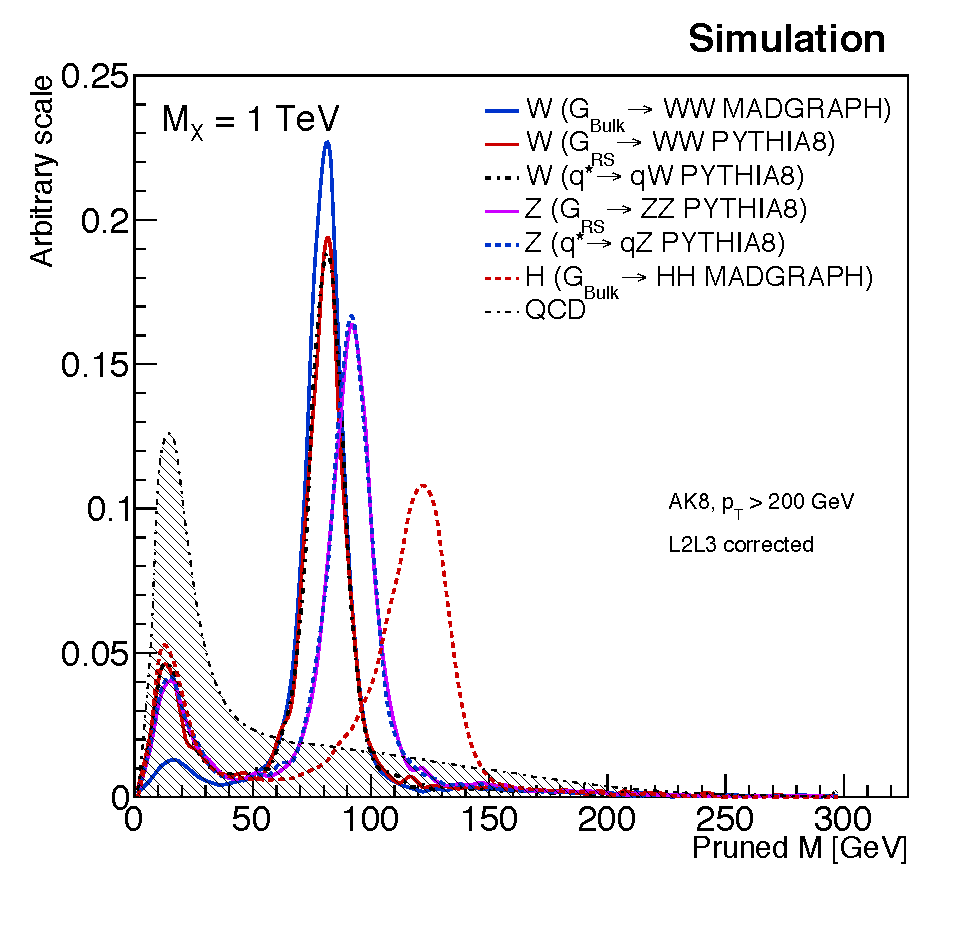
\includegraphics[width=.495\textwidth]{figures/PrunedMass_1TeV.pdf}
    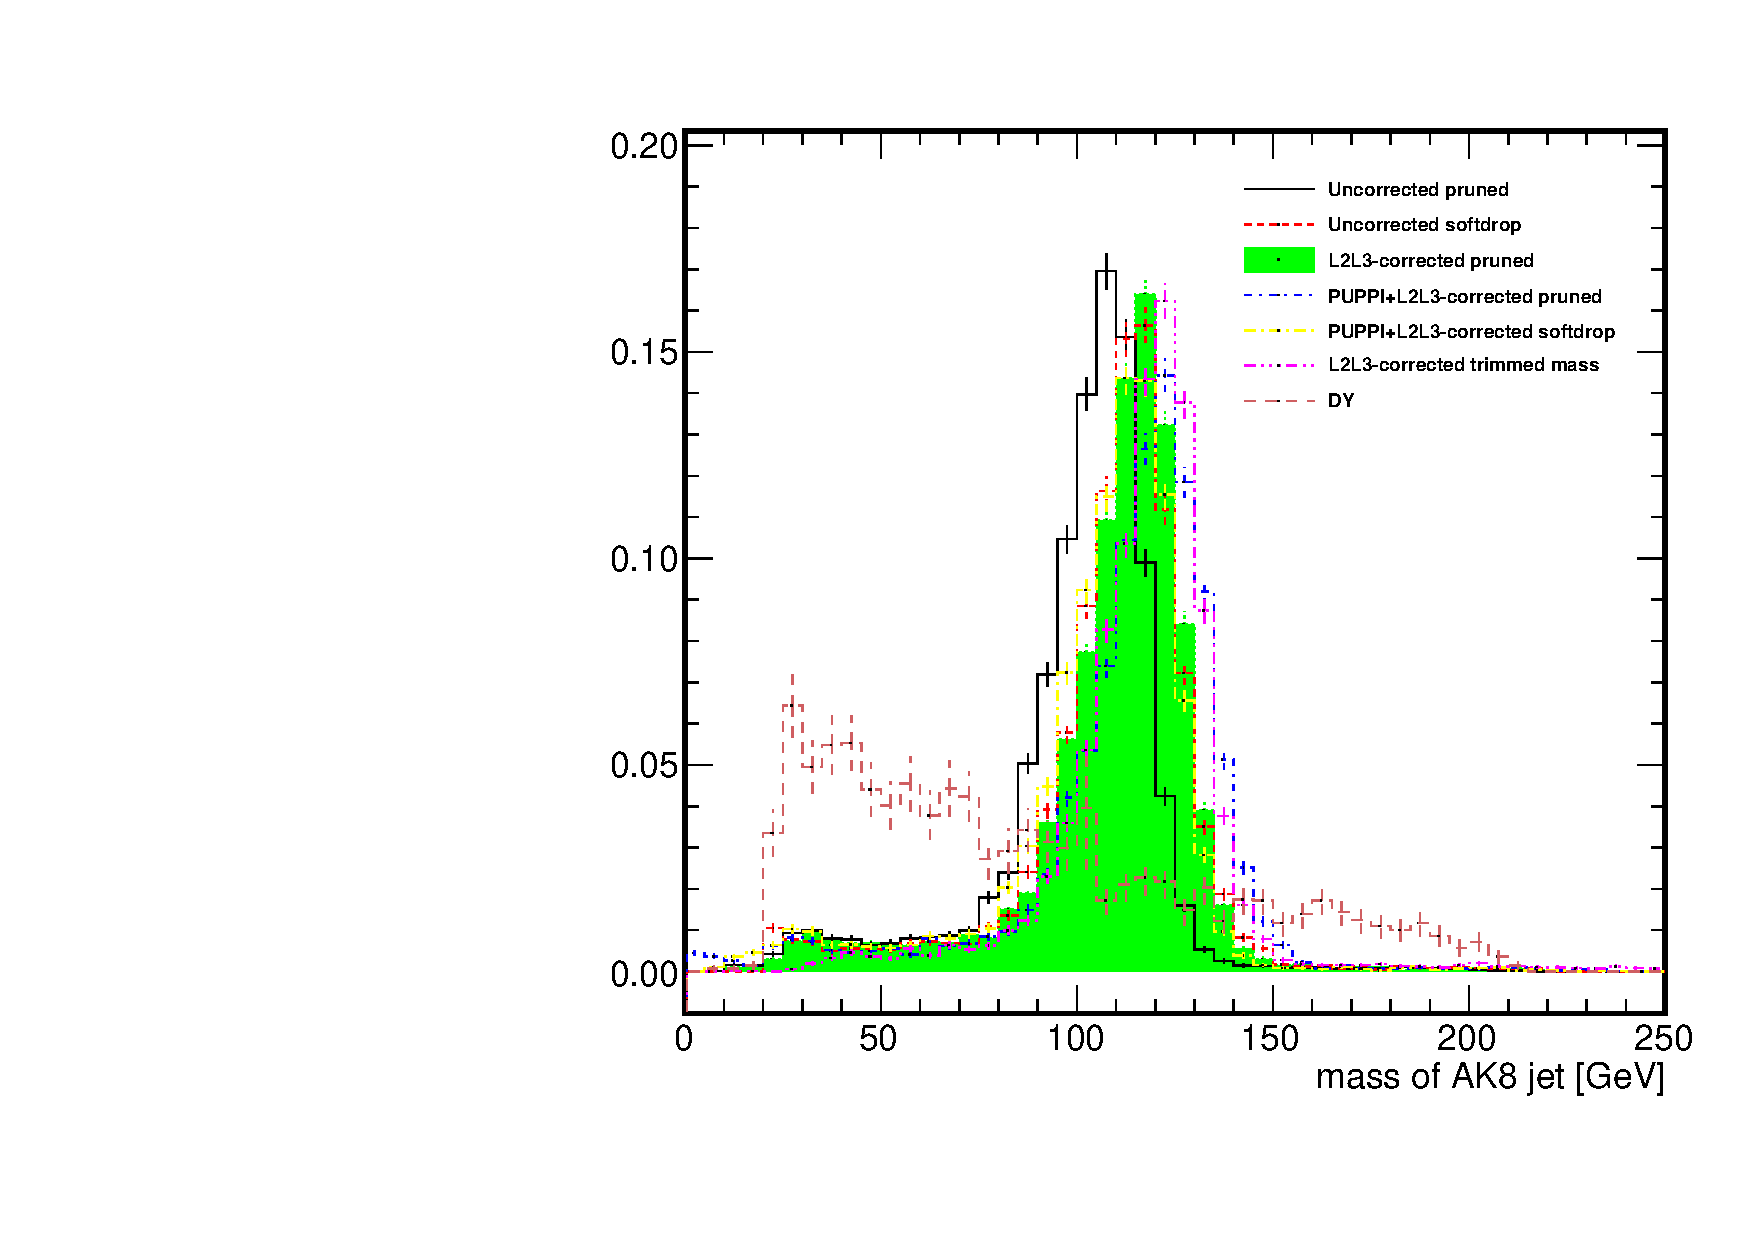
\includegraphics[width=.495\textwidth]{figures/mass2000_distribution.pdf}
  \end{center}
  \caption{\cmsLeft: L2L3-corrected pruned mass for hadronic \PW, \Z and Higgs decays and a resonance mass of 1 \TeV. The shape of the multijet background is also displayed for comparison. \cmsRight: Comparison of the L2L3-corrected pruned mass from the DY+jets 
  background and various mass variables from the 2-TeV Z' signal. These mass 
  variables are computed with various grooming techniques, including softdrop, 
  pruning, and trimming, and two different pileup subtraction methods: charge 
  hadron subtraction (CHS, not explicitly labeled in the figure) and pileup 
  per particle identification (labeled with ``PUPPI'').}  
  \label{fig:allmasses}
\end{figure}

% Why chose


An optimization procedure is then performed to choose the best mass cut window.
 The chosen figure of merit is the \emph{Punzi significance}, which has the 
advantage to be independent on the signal normalization, and is defined as:
%\begin{linenomath}\begin{equation}
$$\mathcal{P} = \frac{\varepsilon_S}{1+\sqrt{B}}$$
%\end{equation}\end{linenomath}
where $\varepsilon_S$ is 
the signal efficiency and $B$ the number of background events. 
Both of them are evaluated  by counting events within a $2\sigma$-width window
in the \mX mass spectrum centered around the peak mean value.
Here, the $\varepsilon_S$ is the signal efficiency with its 
denominator being the number of signal events passing the preselection 
criteria and the $B$ is the number of background events normalized to 
5~\fbinv of integrated luminosity. 
Figure~\ref{fig:sigmass} shows the best Punzi significance and
 its corresponding signal/background efficiencies, as a function of Z' mass. 
Figure~\ref{fig:sigratiomass} shows the ratio of best significance relative 
to the significance when applying a mass cut of 105-135~\GeV 
(common window of the diboson group); in addition, the efficiency ratios are 
also shown. 
Table~\ref{tab:sigratiomass} lists the input numbers of Punzi significance 
for various mass windows and for Z' mass at 1, 2, 3, and 4 TeV respectively.
Overall, about 20--30\% of significance is reduced by using the mass window 
105--135~\GeV. 


\begin{figure}[!htb]
  \begin{center}
    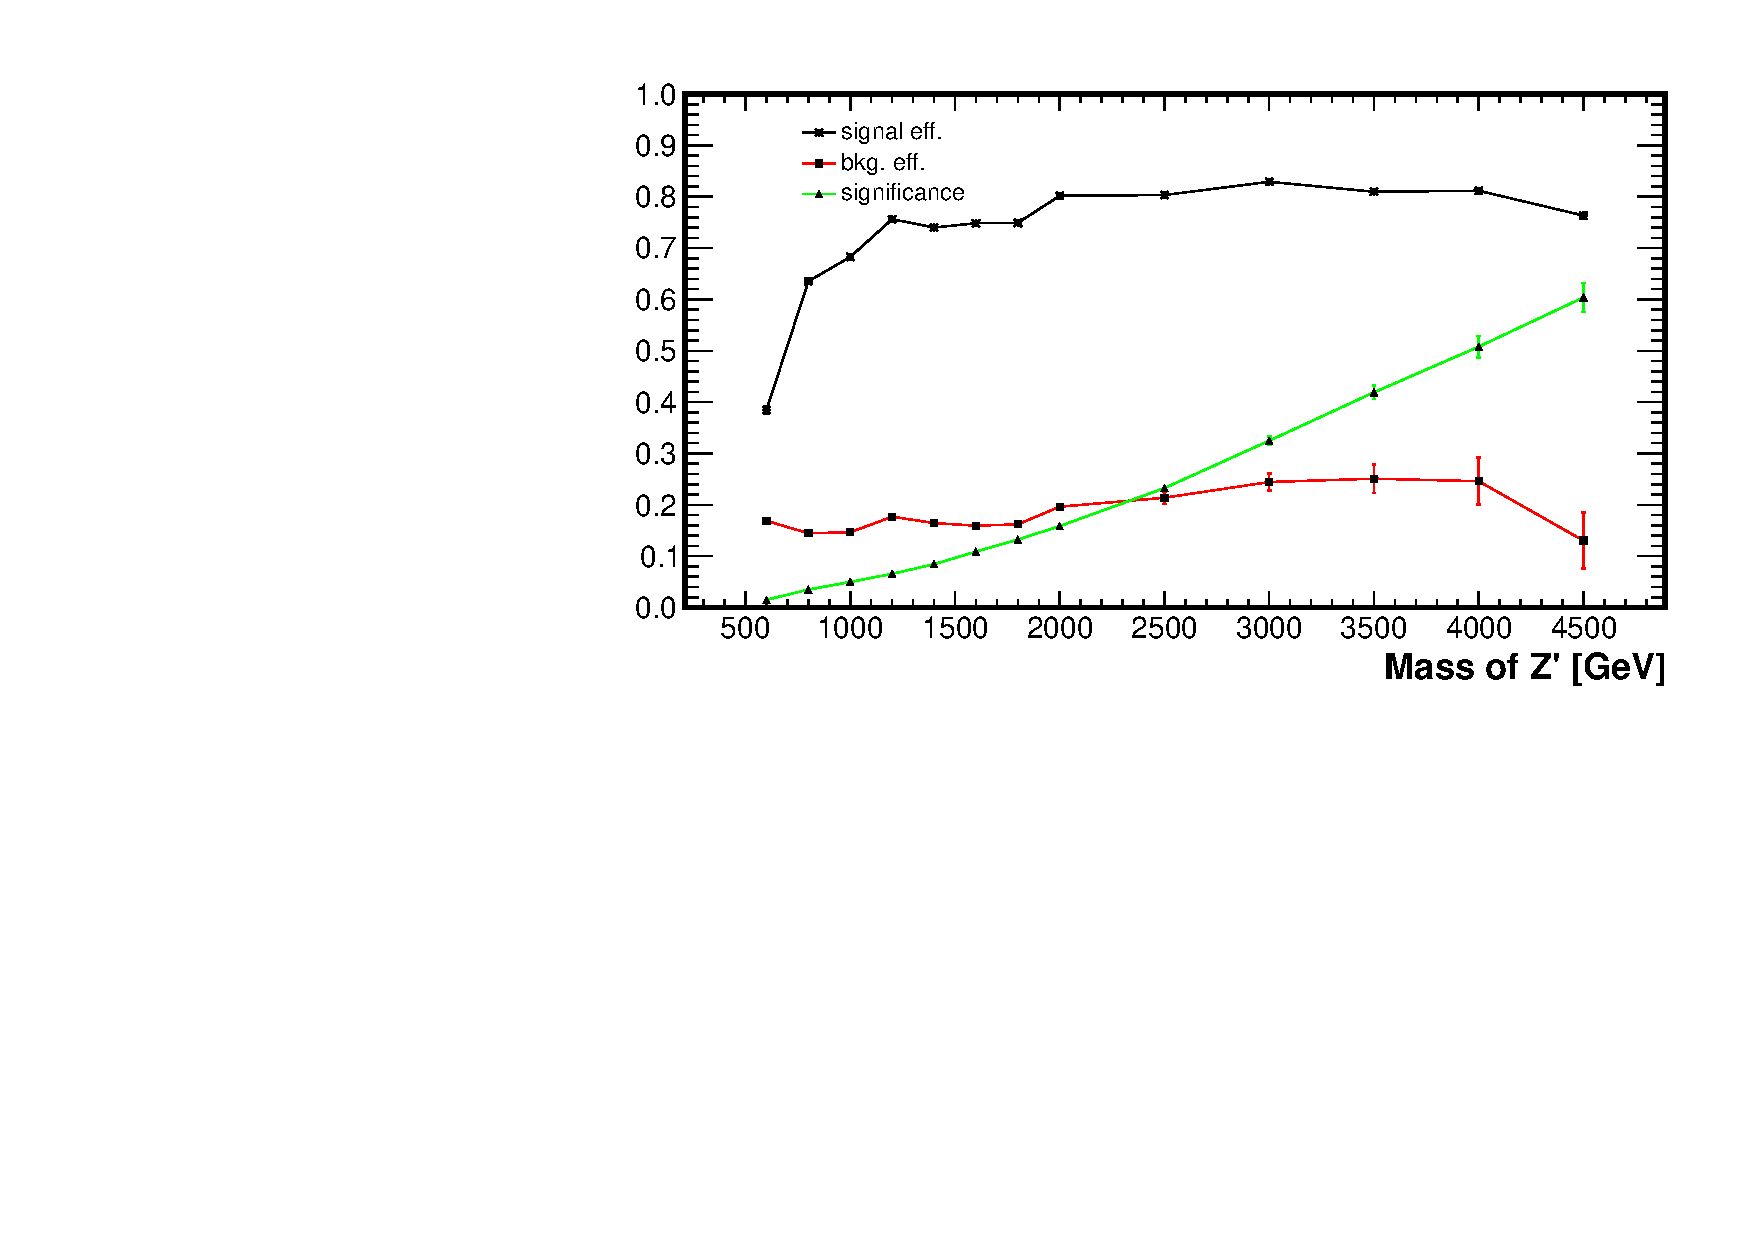
\includegraphics[width=.9\textwidth]{figures/significance.pdf}
  \end{center}
  \caption{The best Punzi significance for the selection on 
L2L3-corrected pruned mass and the corresponding signal/background 
efficiencies, as a function of Z' mass. }  
  \label{fig:sigmass}
\end{figure}


\begin{figure}[!htb]
  \begin{center}
    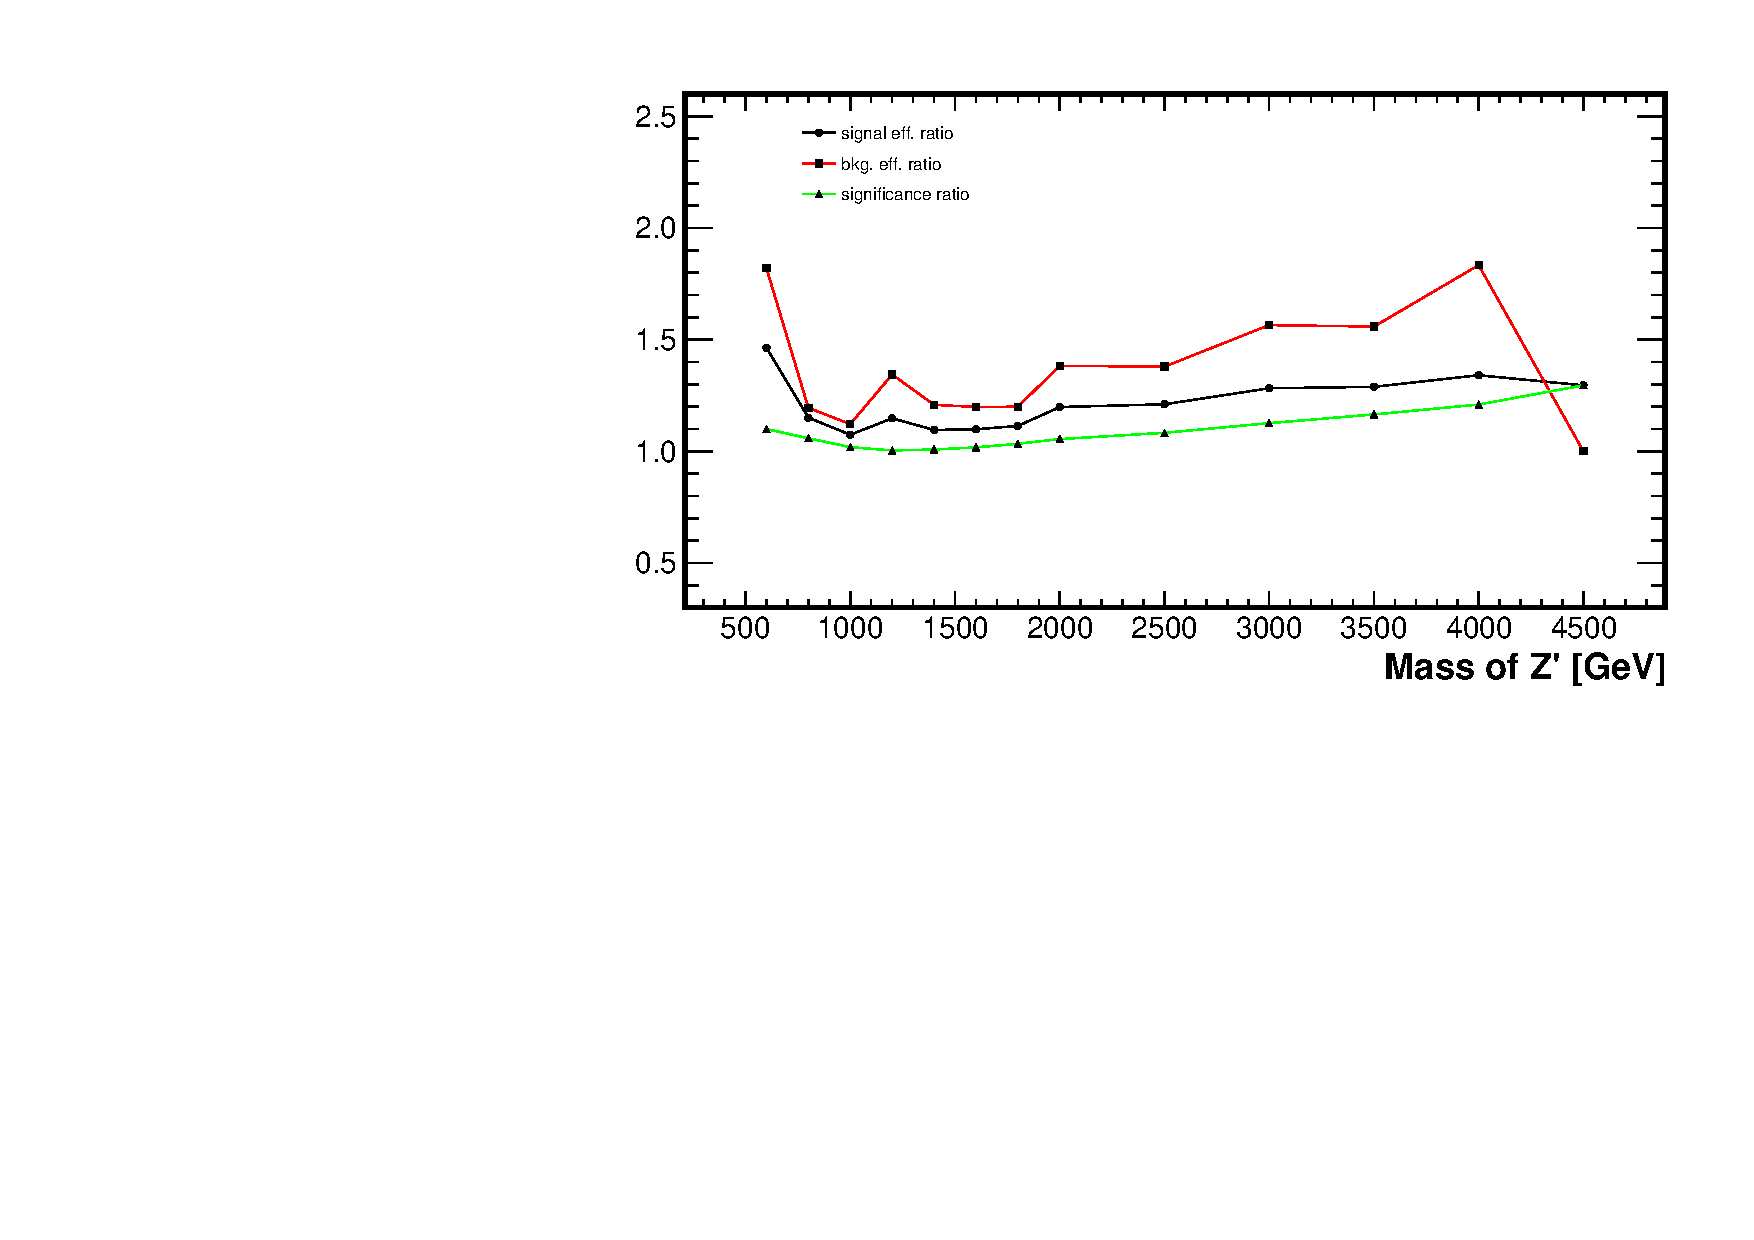
\includegraphics[width=.9\textwidth]{figures/ratio.pdf}
  \end{center}
  \caption{The ratio of the best significance relative to the significance 
 with mass window of 105--135~\GeV,  as a function 
of Z' mass. The corresponding efficiency ratios for the signal 
 and background are also shown. }  
  \label{fig:sigratiomass}
\end{figure}


\begin{table}[!htb]
  \begin{center}
\caption{Punzi significance, the signal efficiency and the number of 
 background events for various mass windows. The numbers in bold font 
 correspond to the mass 
 window with best significance for this analysis. The numbers for the  
 common window 105--135 GeV and the best window for all-hadronic channel 
 are also shown. \label{tab:sigratiomass}}
  \begin{tabular}{c|crrr}
 \hline
 \hline
 $M_{Z'}$ & corr. $M_\mathrm{pruned}$ [\GeV] & $\mathcal{P}$ &  $\varepsilon_S$ & $B$ \\
 \hline
  1 \TeV & {\bf 105--140} & {\bf 0.0498} & {\bf 0.6827} & {\bf 161.6} \\ 
         & 105--135 &  0.0489 & 0.6357 & 144.1 \\
 \hline
  2 \TeV & {\bf 95--135} & {\bf 0.1586} & {\bf 0.8018} & {\bf 16.45} \\
         & 105--135 & 0.1504 & 0.6693 & 11.90 \\
         & 100--130 & 0.1561 & 0.7090 & 12.55 \\
  \hline
  3 \TeV & {\bf 90--135} & {\bf 0.3249} & {\bf 0.8290} & {\bf 2.408} \\
         & 105--135 & 0.2886 & 0.6466 & 1.539 \\
         & 100--130 & 0.3062 & 0.6991 & 1.646 \\
  \hline
  4 \TeV & {\bf 90--145} & {\bf 0.5078} & {\bf 0.8116} & {\bf 0.3580} \\
         & 105--135 & 0.4200 & 0.6055 & 0.1952 \\
         & 95--135 & 0.4903 & 0.7449 & 0.2696 \\
 \hline
 \hline
 \end{tabular}
 \end{center}
\end{table}



\subsubsection*{Optimization of electron kinematic selection criteria \label{sec:opt_ele}}

In this section, we study the best selection on the \pt's of leading and 
sub-leading electrons, respectively. Particularly, given that the minimum \pt 
threshold of leading electron is limited by the single electron trigger, we 
would like to see how low we could go in the \pt of sub-leading electron. 
The chosen figure of merit is the ``Punzi 
significance'', which has the advantage to be independent of the signal 
normalization and is defined as:
\[\mathcal{P} = \frac{\varepsilon_S}{1+\sqrt{B}}.\] 
Here, the $\varepsilon_S$ is the signal efficiency with its 
denominator being the number of signal 
events passing the preselection criteria in Table~\ref{tab:preselection}, 
and the $B$ is the number of 
background events normalized to 1~\fbinv of integrated luminosity. 
When optimizing the selection on the \pt of sub-leading electron, the 
requirement of ``$\pt^\mathrm{sub}$ $>35$~GeV'' is removed.

Figures~\ref{fig:leadptone}--\ref{fig:leadptthree} show (i) the signal and 
background distributions of the $\pt$ of leading electron, and (ii) the Punzi 
significance, signal and background efficiencies as a function of minimum \pt 
thresholds, for Z' mass at 1, 2, and 3 TeV, respectively. 
Figure~\ref{fig:leadptmass} shows, as a function of Z' mass, (i) the best 
Punzi significance, its corresponding signal/background efficiencies, and 
(ii) the ratio of best significance relative to the significance with 
preselection only. 
Although an improvement of 1--14\% of significance 
could be gained by applying a \pt threshold tighter than the preselection 
(at 115~\GeV), one also see that the threshold strongly depends on the Z' 
mass and the best selection corresponds to about 1/4 of the Z' mass. 

Figures~\ref{fig:subptone}--\ref{fig:subptthree} show (i) the signal and 
background distributions of the $\pt$ of sub-leading electron, and (ii) the 
Punzi significance, signal and background efficiencies as a function of 
minimum \pt thresholds, for Z' mass at 1, 2, and 3 TeV, respectively. 
Figure~\ref{fig:subptmass} shows, as a function of Z' mass, (i) the best Punzi 
significance, its corresponding signal/background efficiencies, and (ii) the 
ratio of best significance relative to the significance with preselection 
only. 
The improvement is at most 5~\%. Therefore, we choose to stay with the 
preselection \pt threshold. 

Note that due to the small size of simulated samples, very few background 
events satisfy the preselection, particularly the $M_{Zh}$ requirement. 
For example, only one DY+jets 
background event survives the pre-selection for the optimization at 
$M_{Z'}=$4.5~TeV. 



\begin{table}[!htb]
  \begin{center}
\caption{Pre-selection for the $X \to Zh$ analysis. \label{tab:preselection}}
  \begin{tabular}{cl}
\hline\hline
 Physics Quantity & Cut Value \\
\hline
 HLT Path & {\sc HLT\_Ele105\_CaloIdVT\_GsfTrkIdT\_*} \\
 Good vertex & $\geq 1$  \\
\hline
\multicolumn{2}{c}{Electron}\\
\hline
 supercluster $\eta$ &  $\left|\eta_\mathrm{SC}\right| < 1.4442$ or $1.566 < \left|\eta_\mathrm{SC}\right| < 2.5$  \\
 ID & HEEP NOISO v6.0  \\
 miniIso & $<0.1$  \\
\hline
\multicolumn{2}{c}{Di-electron pair}\\
 \hline
 $\pt^\mathrm{lead}$ & $>115$~GeV  \\
 $\pt^\mathrm{sub}$ & $>35$~GeV  \\
 Oppositely charged & Yes  \\ 
 $M_{\ell\ell}$ & 70--110 GeV  \\ 
 $\pt^{\ell\ell}$ & $>200$~GeV  \\
\hline
\multicolumn{2}{c}{AK8 jet}\\
 \hline
 $\Delta R(e,j)$ &  $>0.8$ \\
 \pt & $>200$~GeV \\
 $\left|\eta\right|$ & $<2.4$ \\
 Uncorrected pruned mass & 95--130 GeV \\
 \hline
 $M_{Zh}$ & $\pm 15\%$ of mean \\
\hline\hline
 \end{tabular}
 \end{center}
\end{table}


%%%%%%%%%%%%%%%%%%%%%%%%%%%%%%%% leading electron pt

\begin{figure}[htbp]
   \centering
   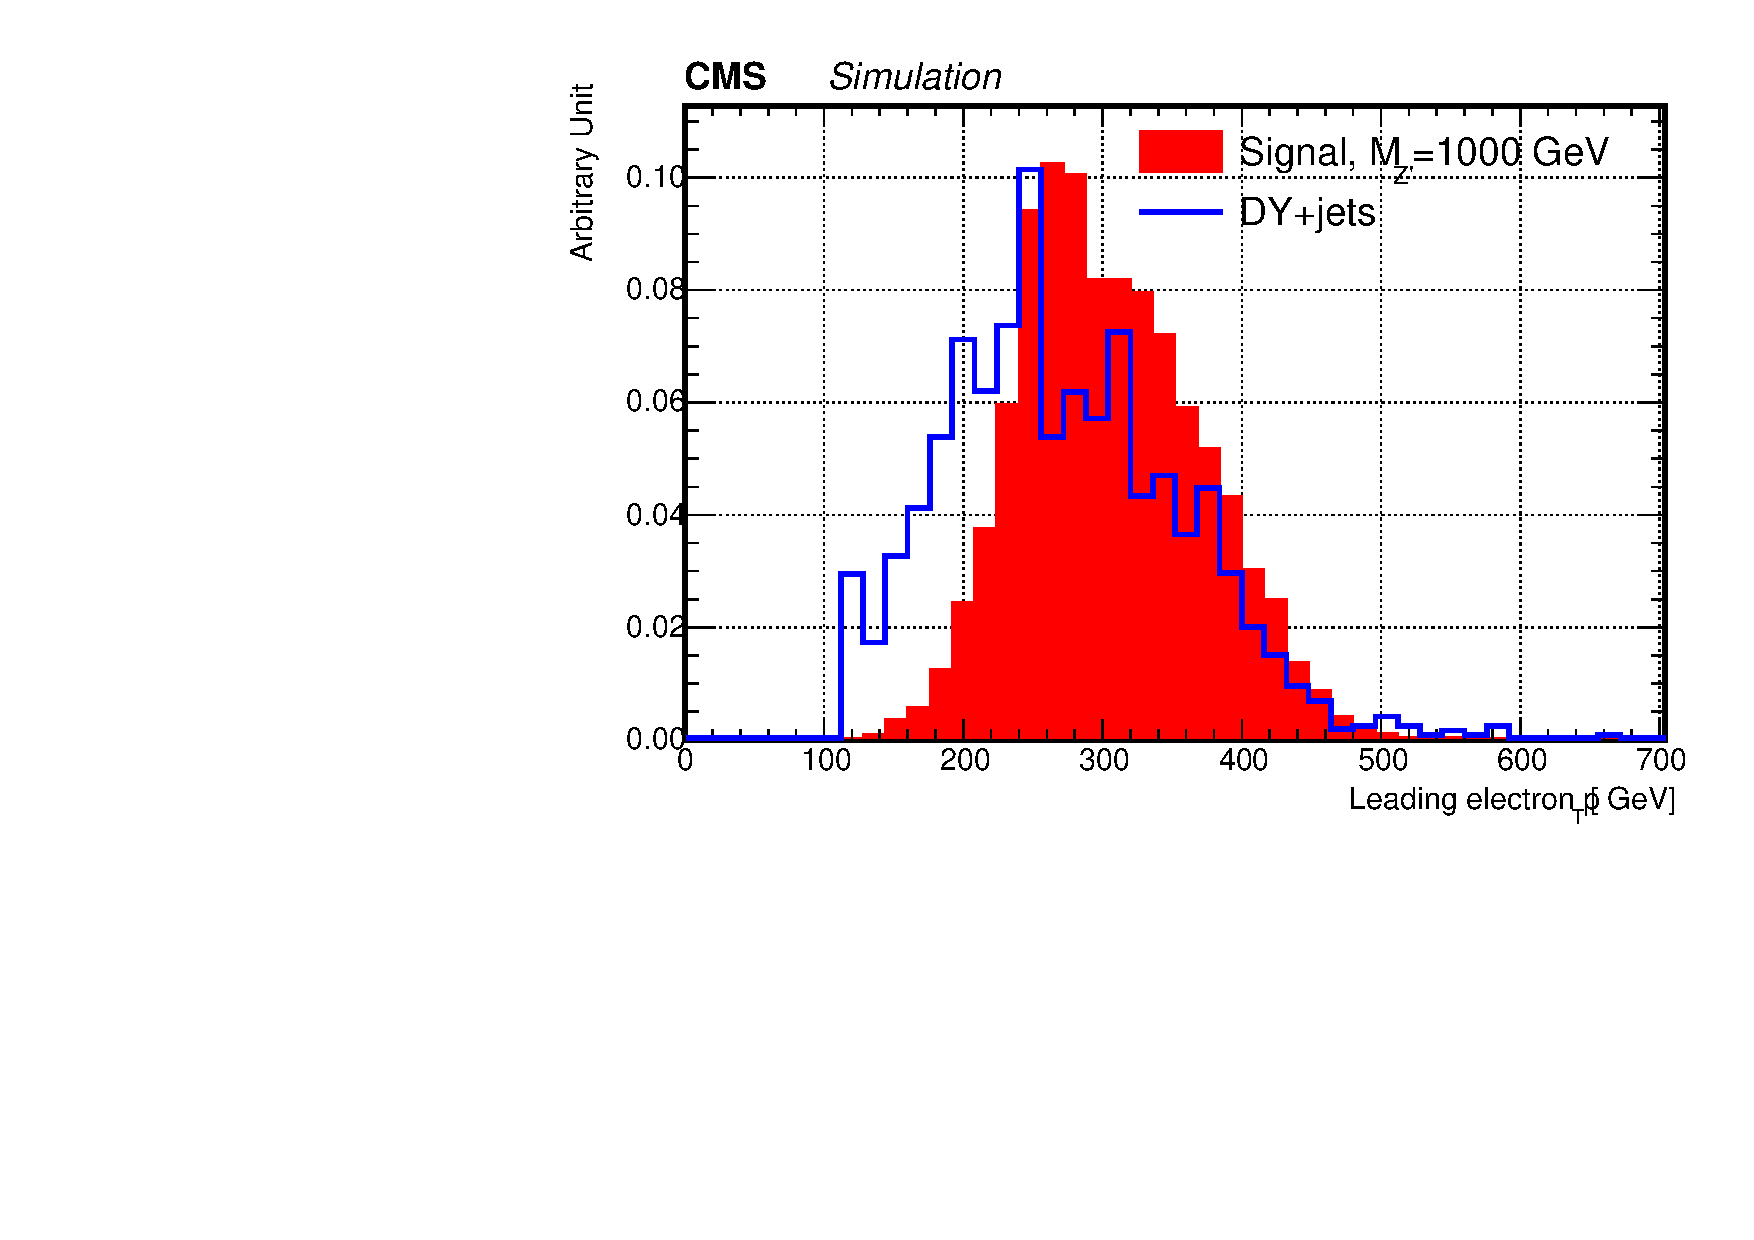
\includegraphics[width=0.45\textwidth]{optimization/plot_1st_pt/plot_1st_pt_input_in_Zprime_mass_1000.pdf}
   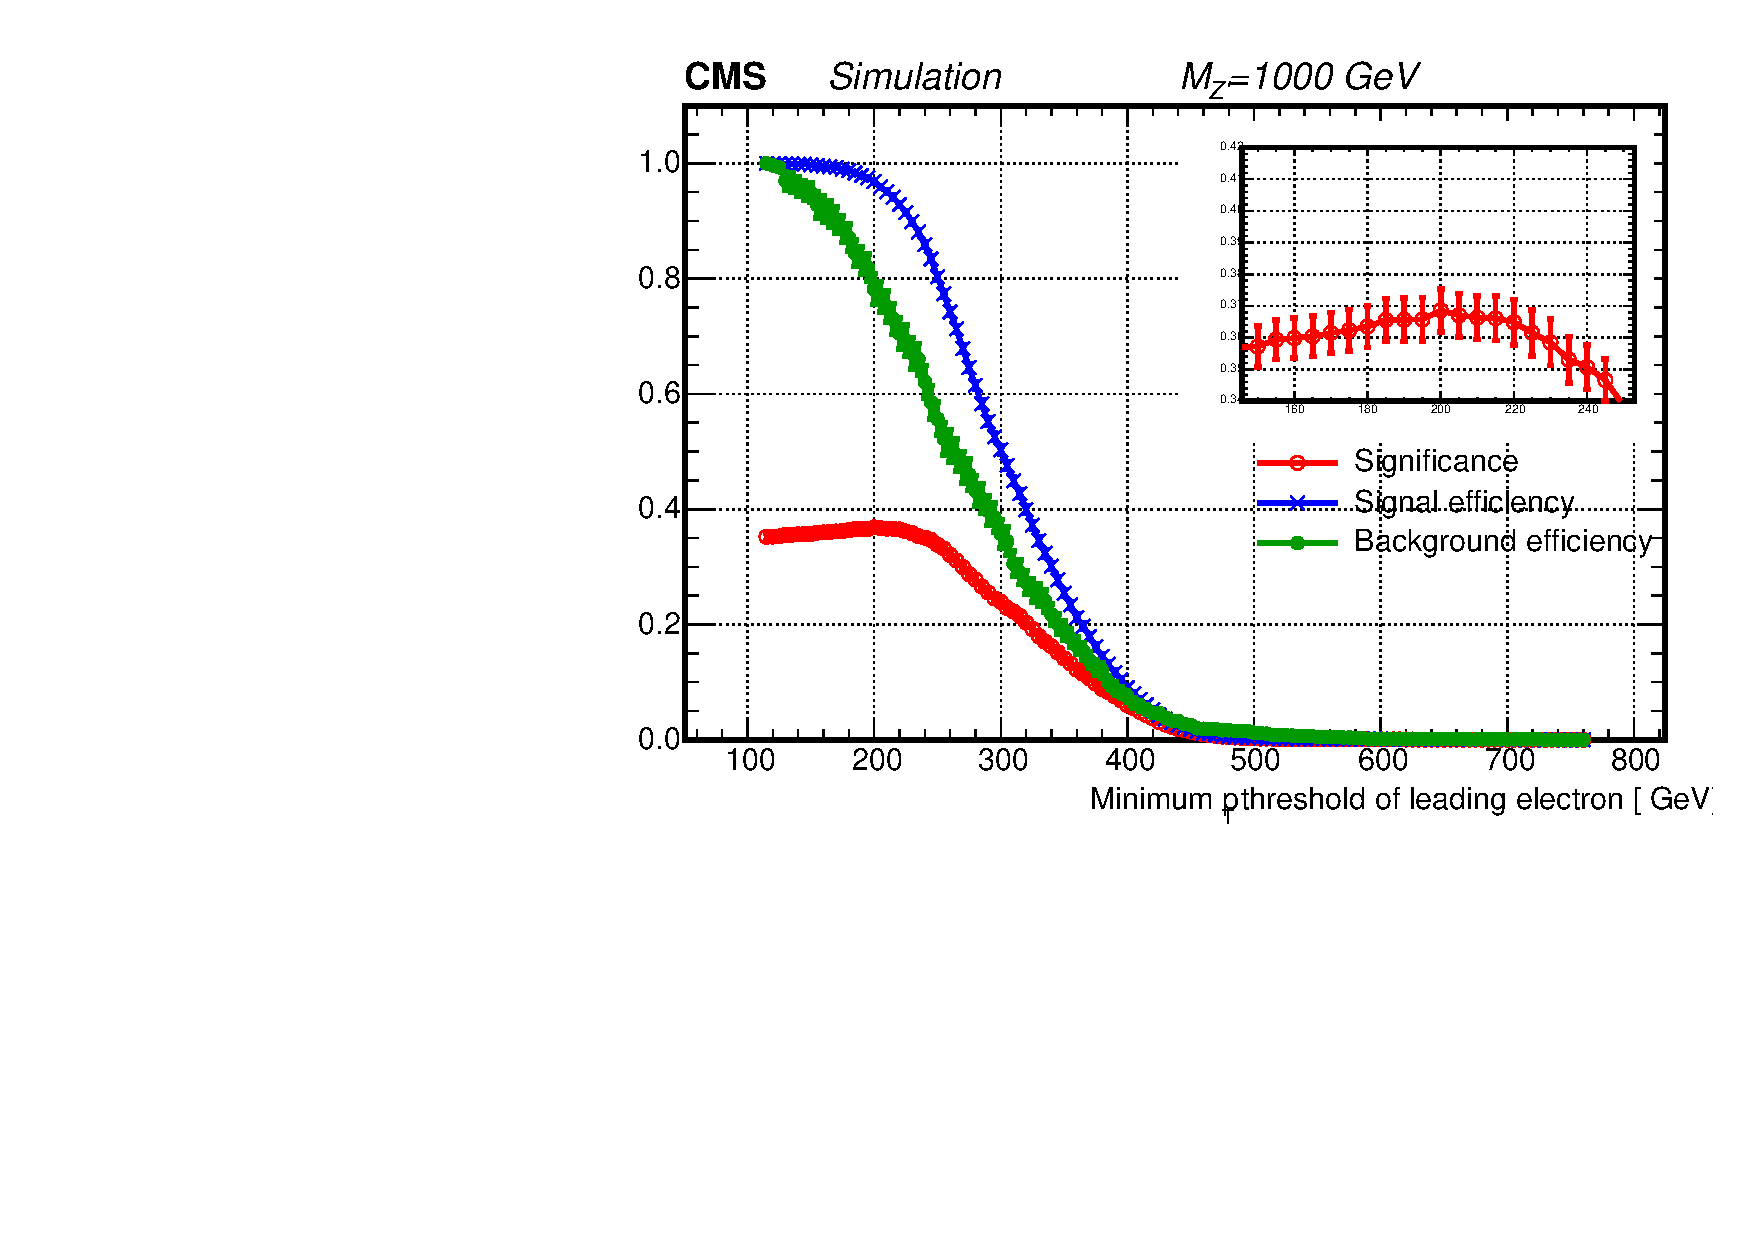
\includegraphics[width=0.45\textwidth]{optimization/plot_1st_pt/plot_1st_pt_Significance_and_efficiency_for_Zprme_M_1000.pdf}
   \caption{The signal and background distributions of leading electron \pt 
(left) and the Punzi significance, the signal, and the background efficiencies as a 
 function of minimum \pt threshold (right). The Z' mass is set to 1 TeV. The 
   signal and background distributions on the left are normalized to the same 
   integrated area. The uncertainties on the right are correlated between 
 different bins.}
   \label{fig:leadptone}
\end{figure}

\begin{figure}[htbp]
   \centering
   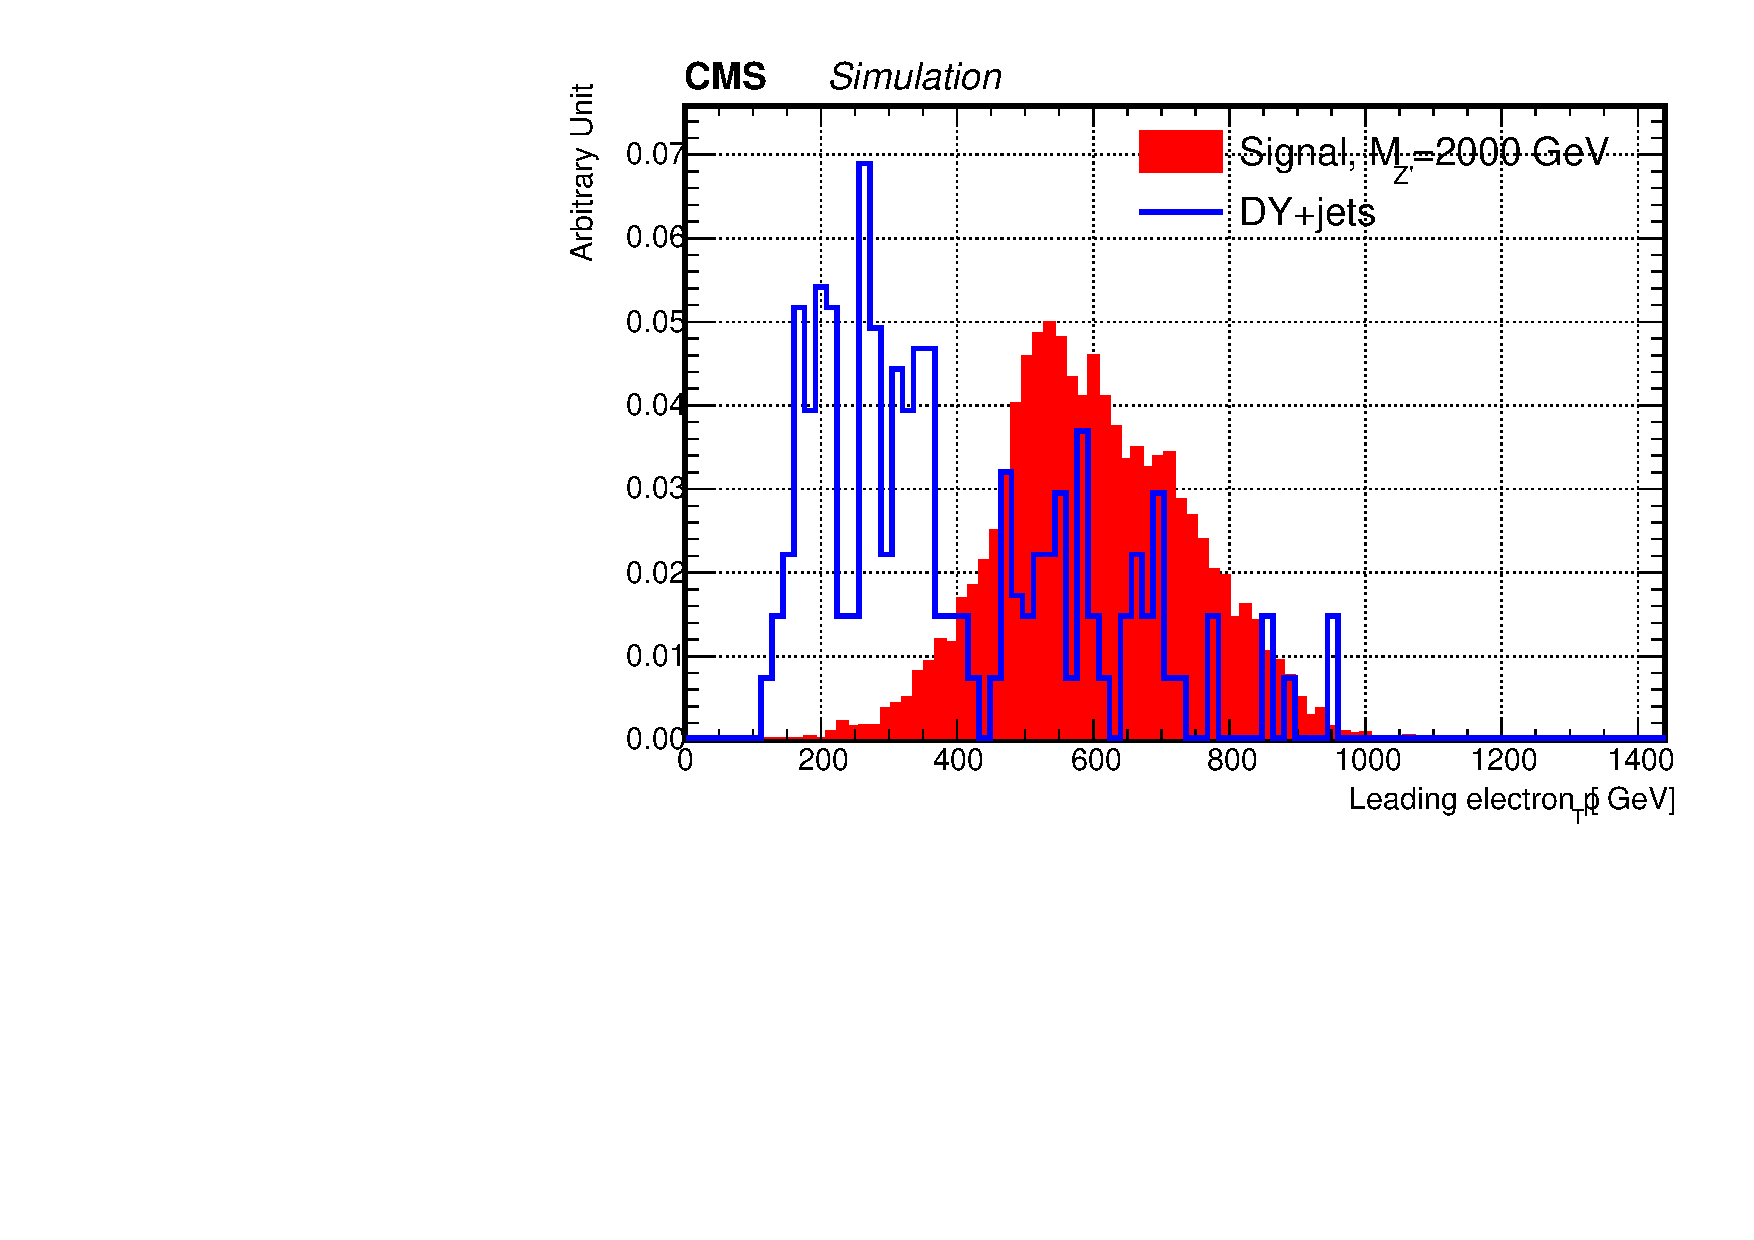
\includegraphics[width=0.45\textwidth]{optimization/plot_1st_pt/plot_1st_pt_input_in_Zprime_mass_2000.pdf}
   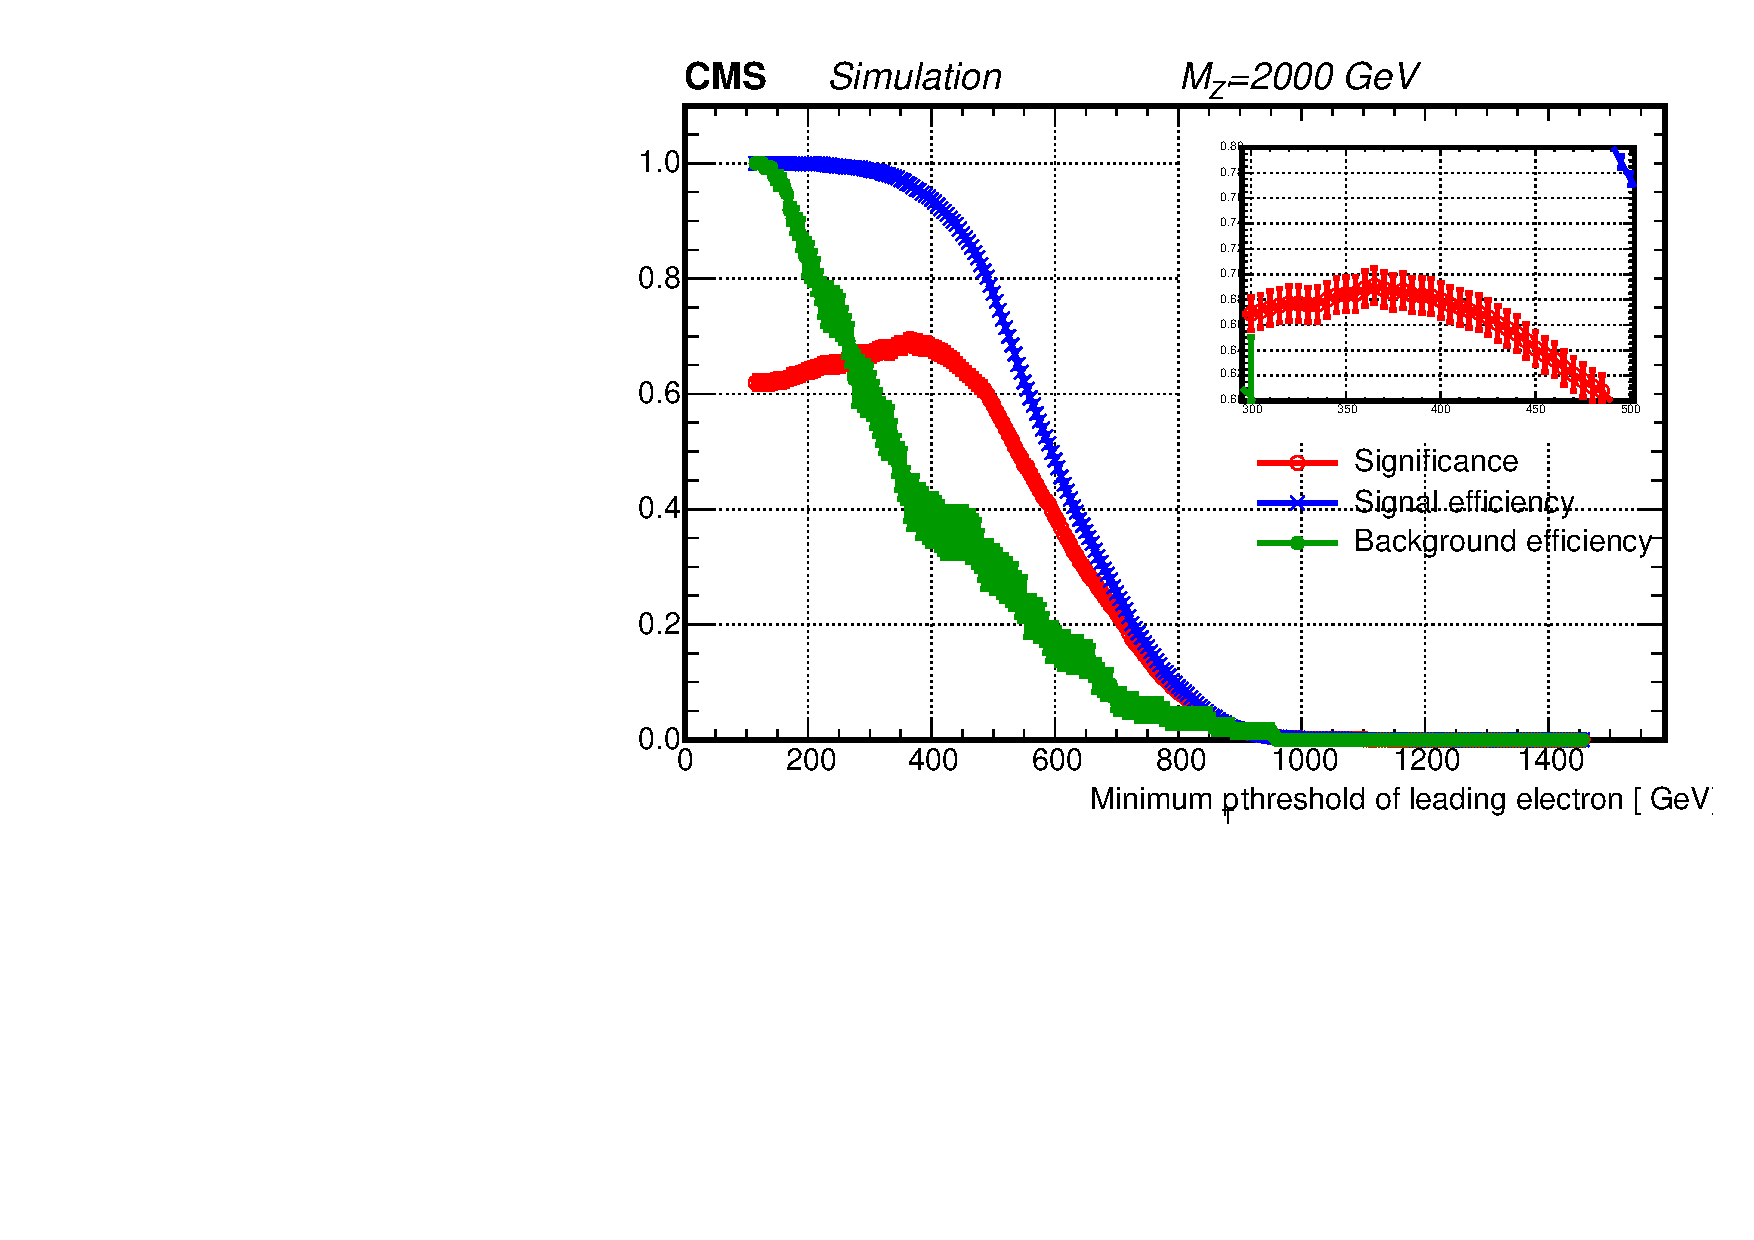
\includegraphics[width=0.45\textwidth]{optimization/plot_1st_pt/plot_1st_pt_Significance_and_efficiency_for_Zprme_M_2000.pdf}
   \caption{The signal and background distributions of leading electron \pt 
(left) and the Punzi significance, the signal, and the background efficiencies as a 
 function of minimum \pt threshold (right). The Z' mass is set to 2 TeV. The 
   signal and background distributions on the left are normalized to the same 
   integrated area. The uncertainties on the right are correlated between 
 different bins.}
   \label{fig:leadpttwo}
\end{figure}

\begin{figure}[htbp]
   \centering
   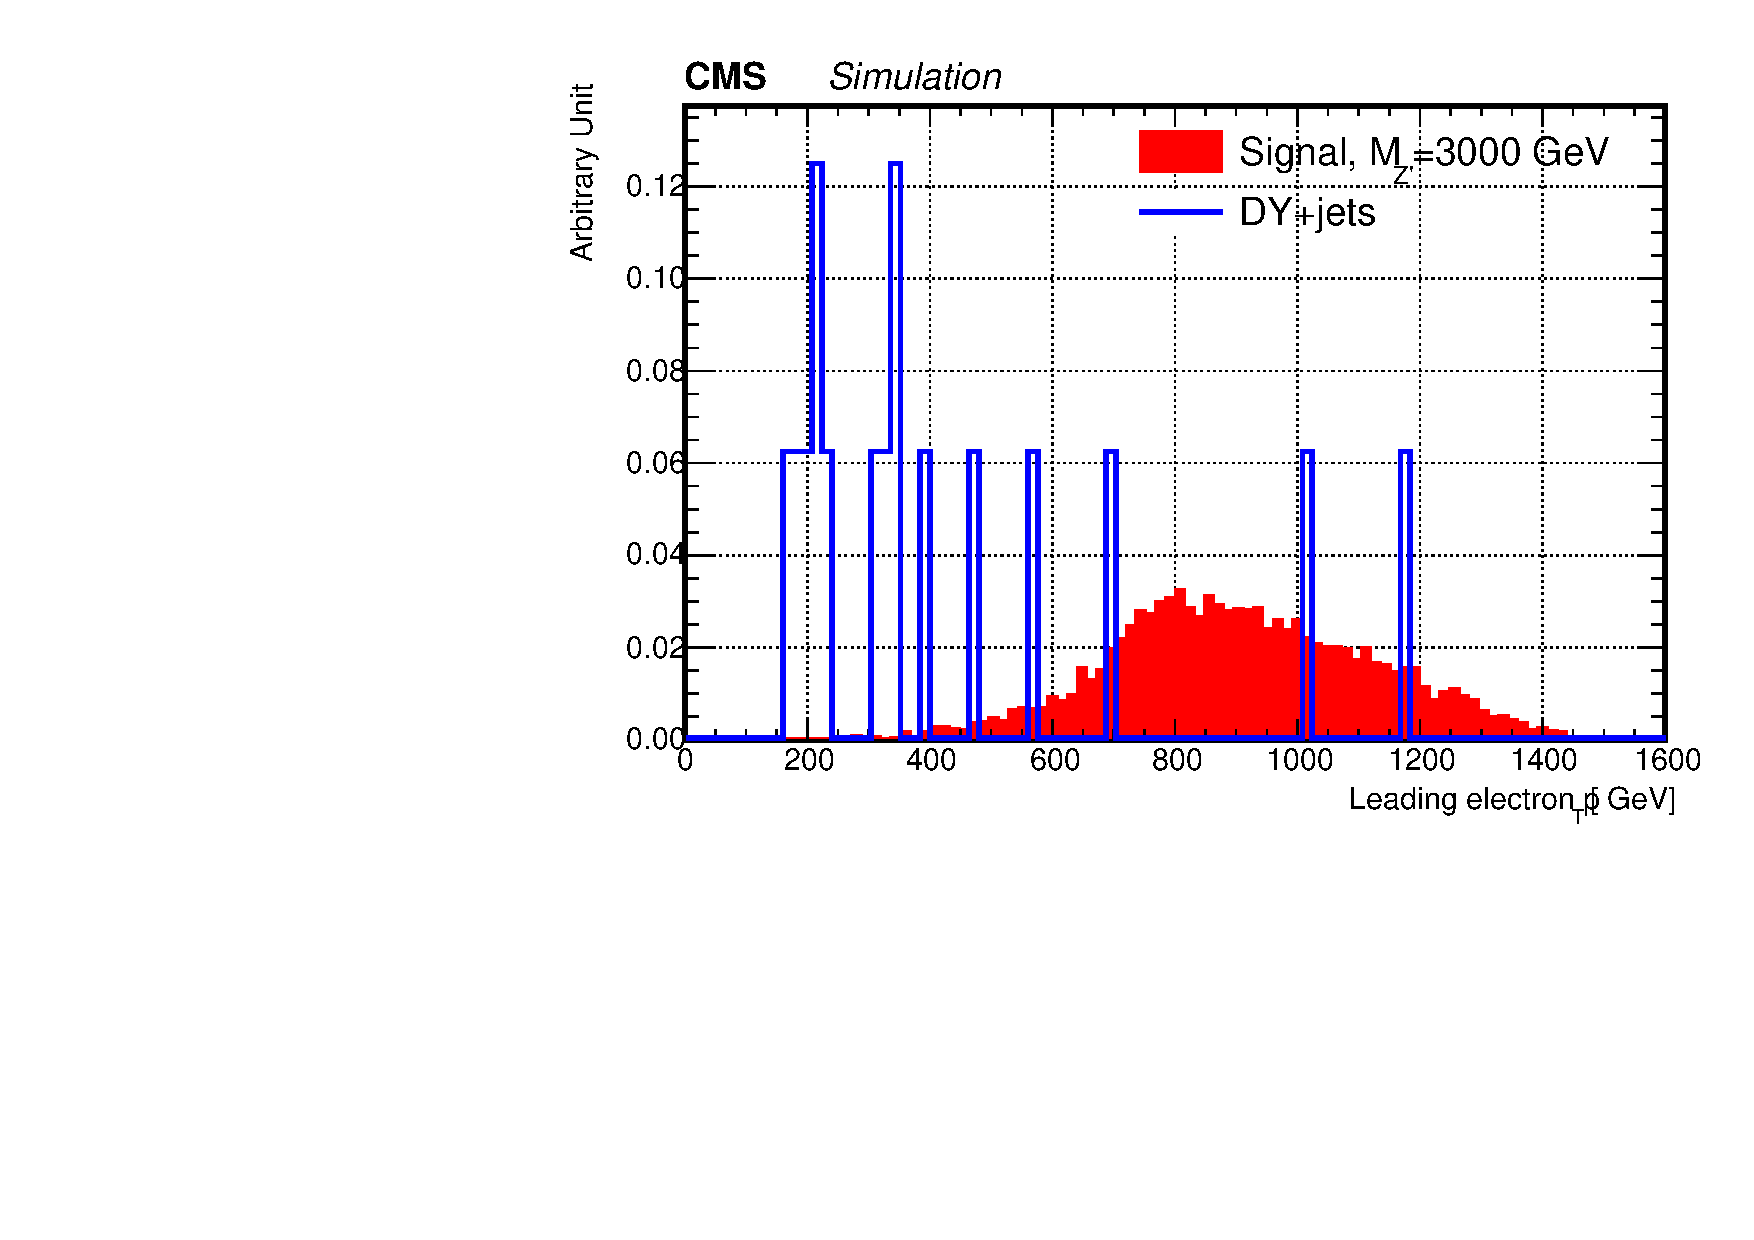
\includegraphics[width=0.45\textwidth]{optimization/plot_1st_pt/plot_1st_pt_input_in_Zprime_mass_3000.pdf}
   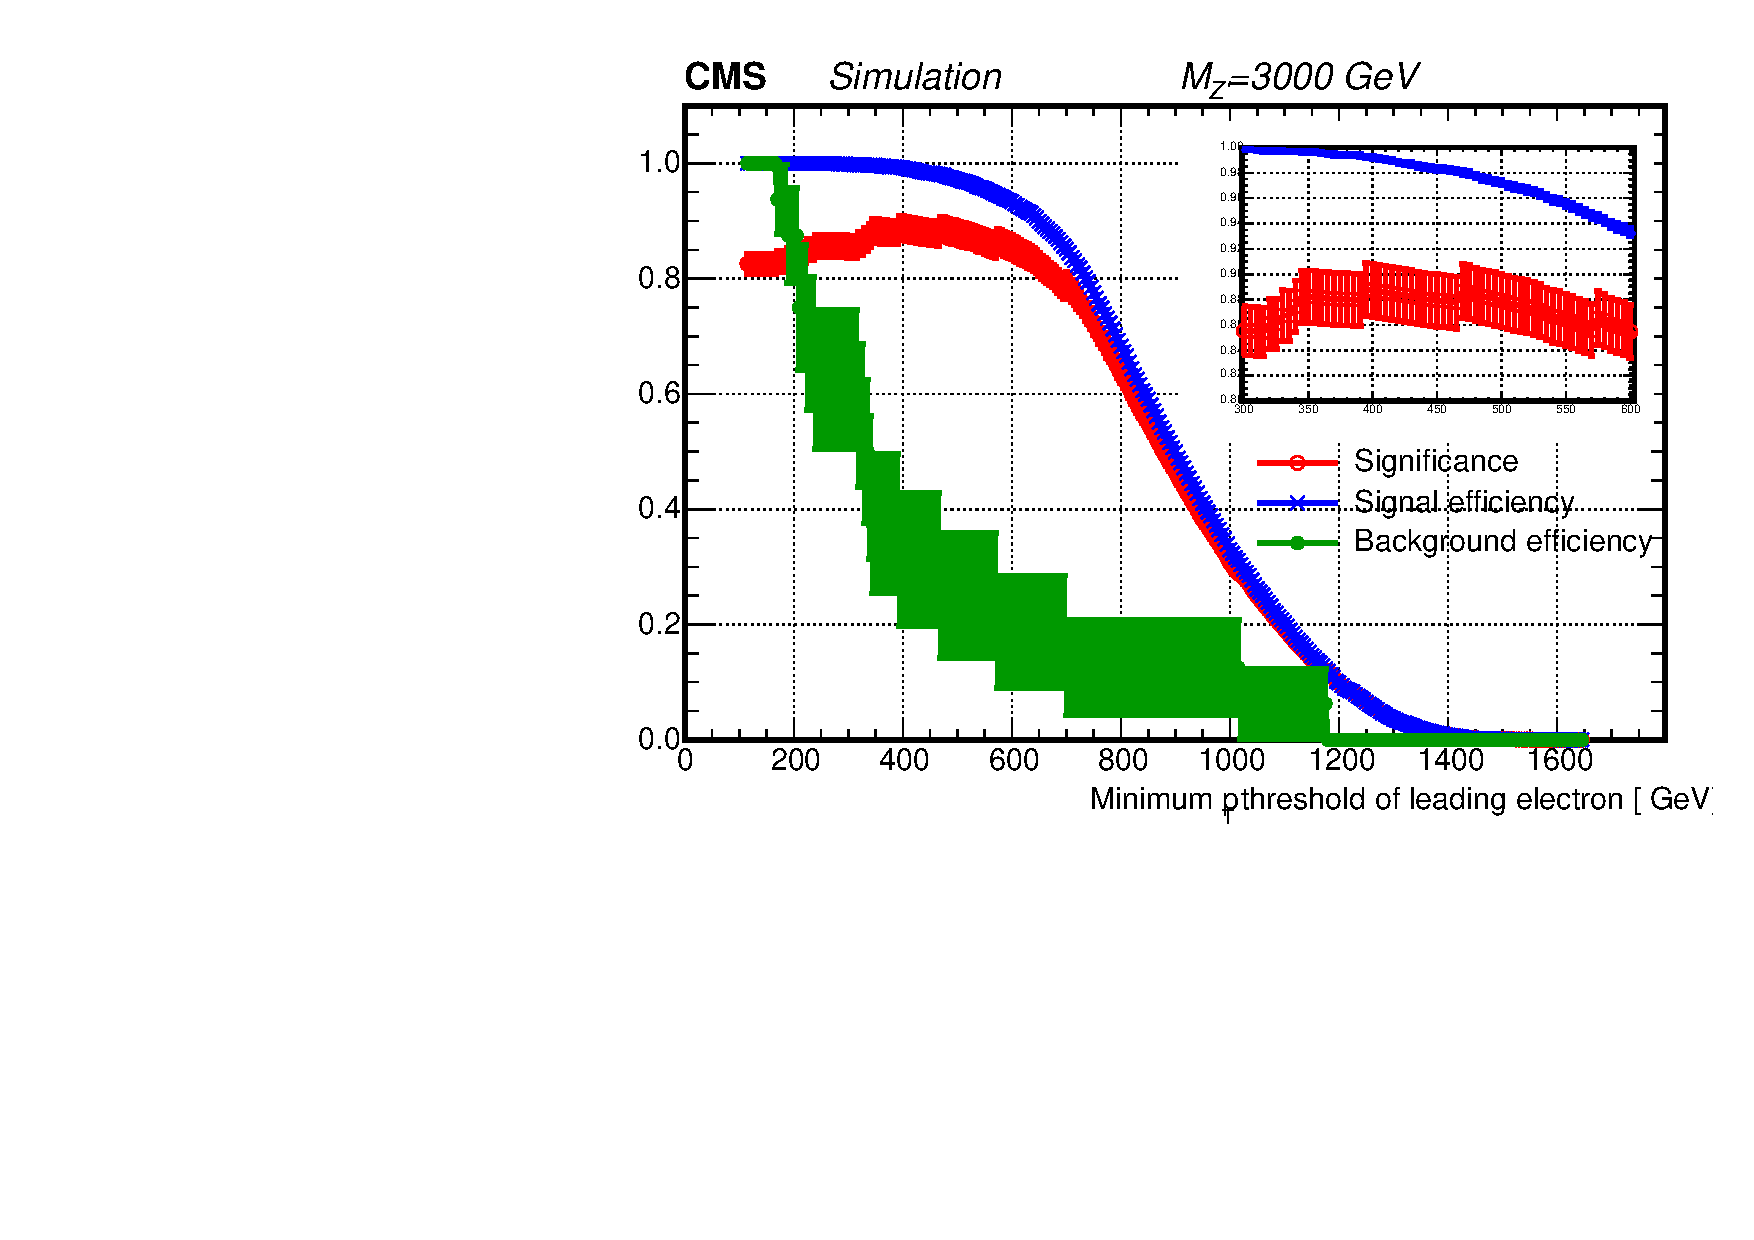
\includegraphics[width=0.45\textwidth]{optimization/plot_1st_pt/plot_1st_pt_Significance_and_efficiency_for_Zprme_M_3000.pdf}
   \caption{The signal and background distributions of leading electron \pt 
(left) and the Punzi significance, the signal, and the background efficiencies as a 
 function of minimum \pt threshold (right). The Z' mass is set to 3 TeV. The 
   signal and background distributions on the left are normalized to the same 
   integrated area. The uncertainties on the right are correlated between 
 different bins.}
   \label{fig:leadptthree}
\end{figure}


\begin{figure}[htbp]
   \centering
   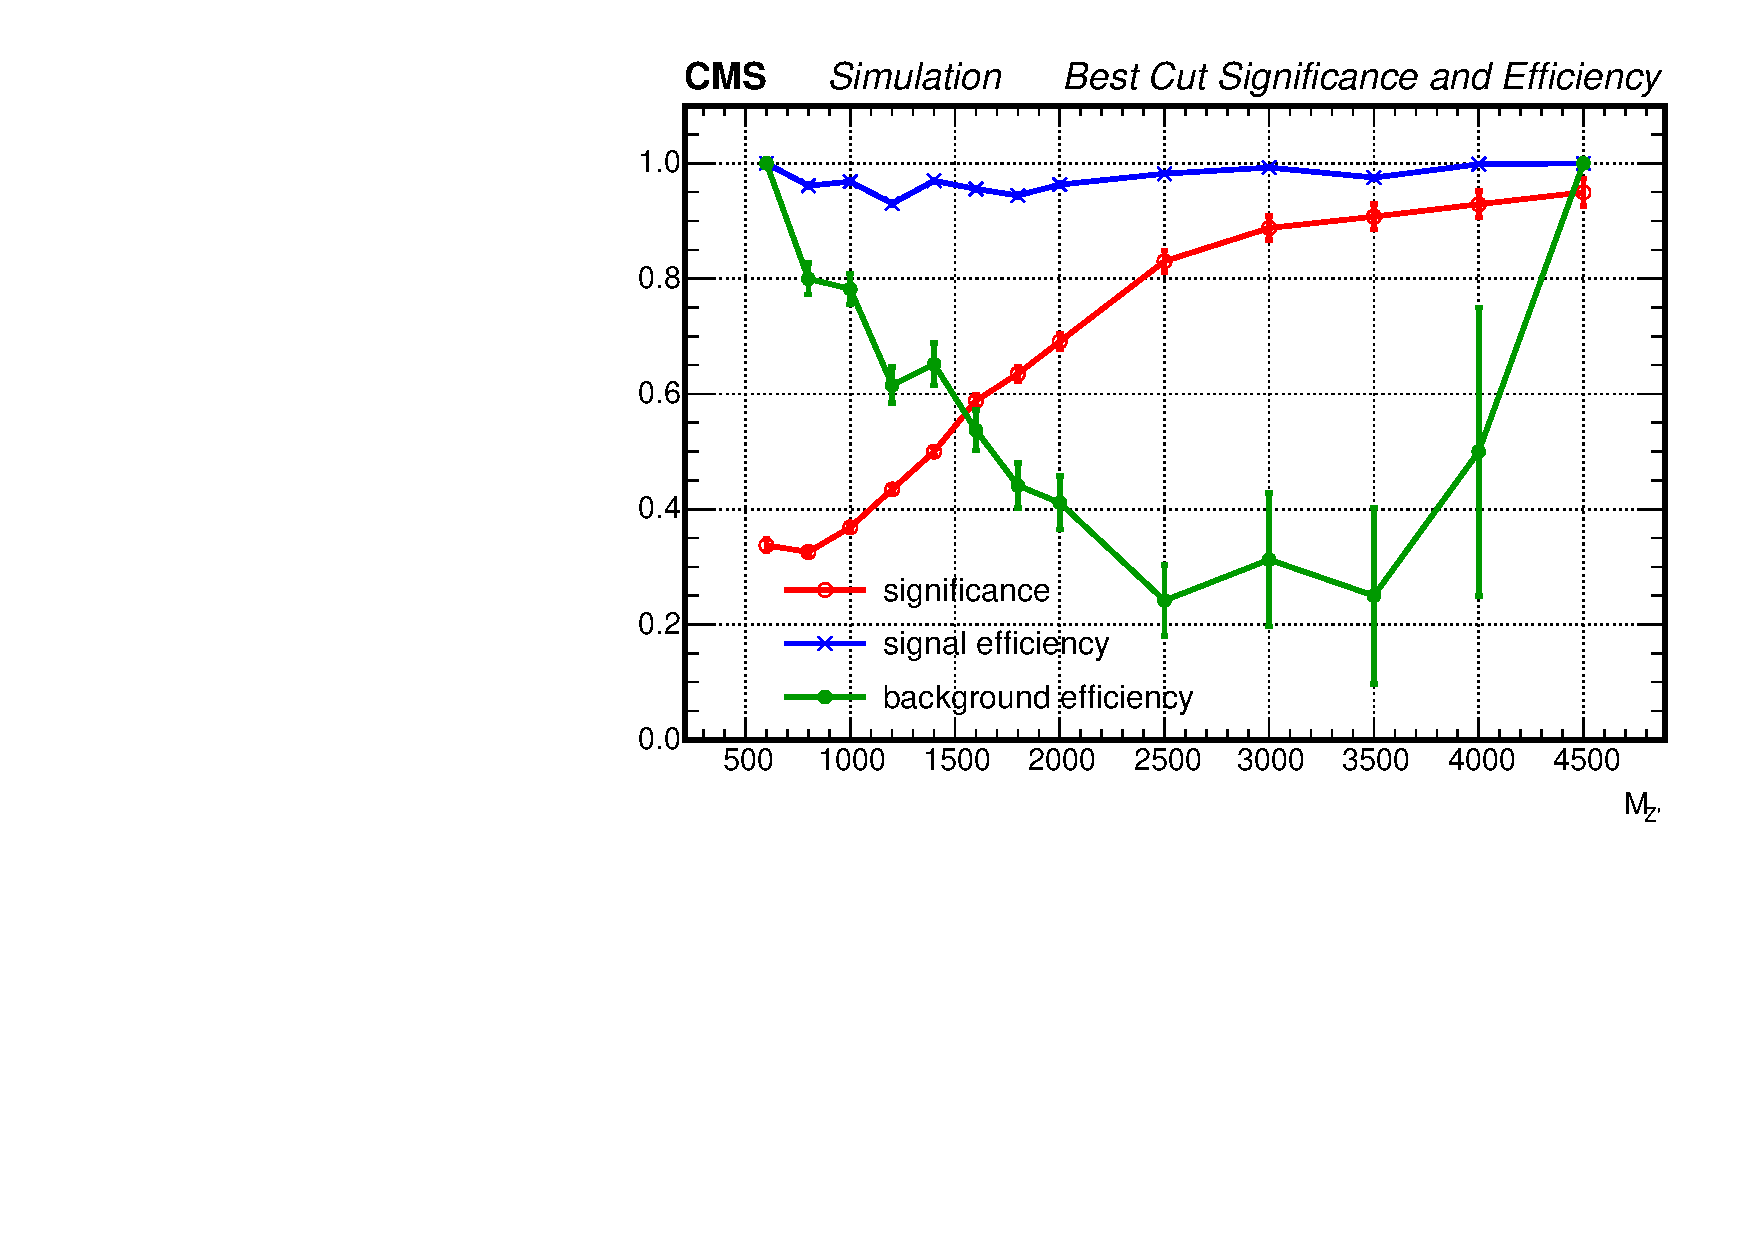
\includegraphics[width=0.45\textwidth]{optimization/plot_1st_pt/plot_1st_pt_best_cut_significance_and_efficiency.pdf}
   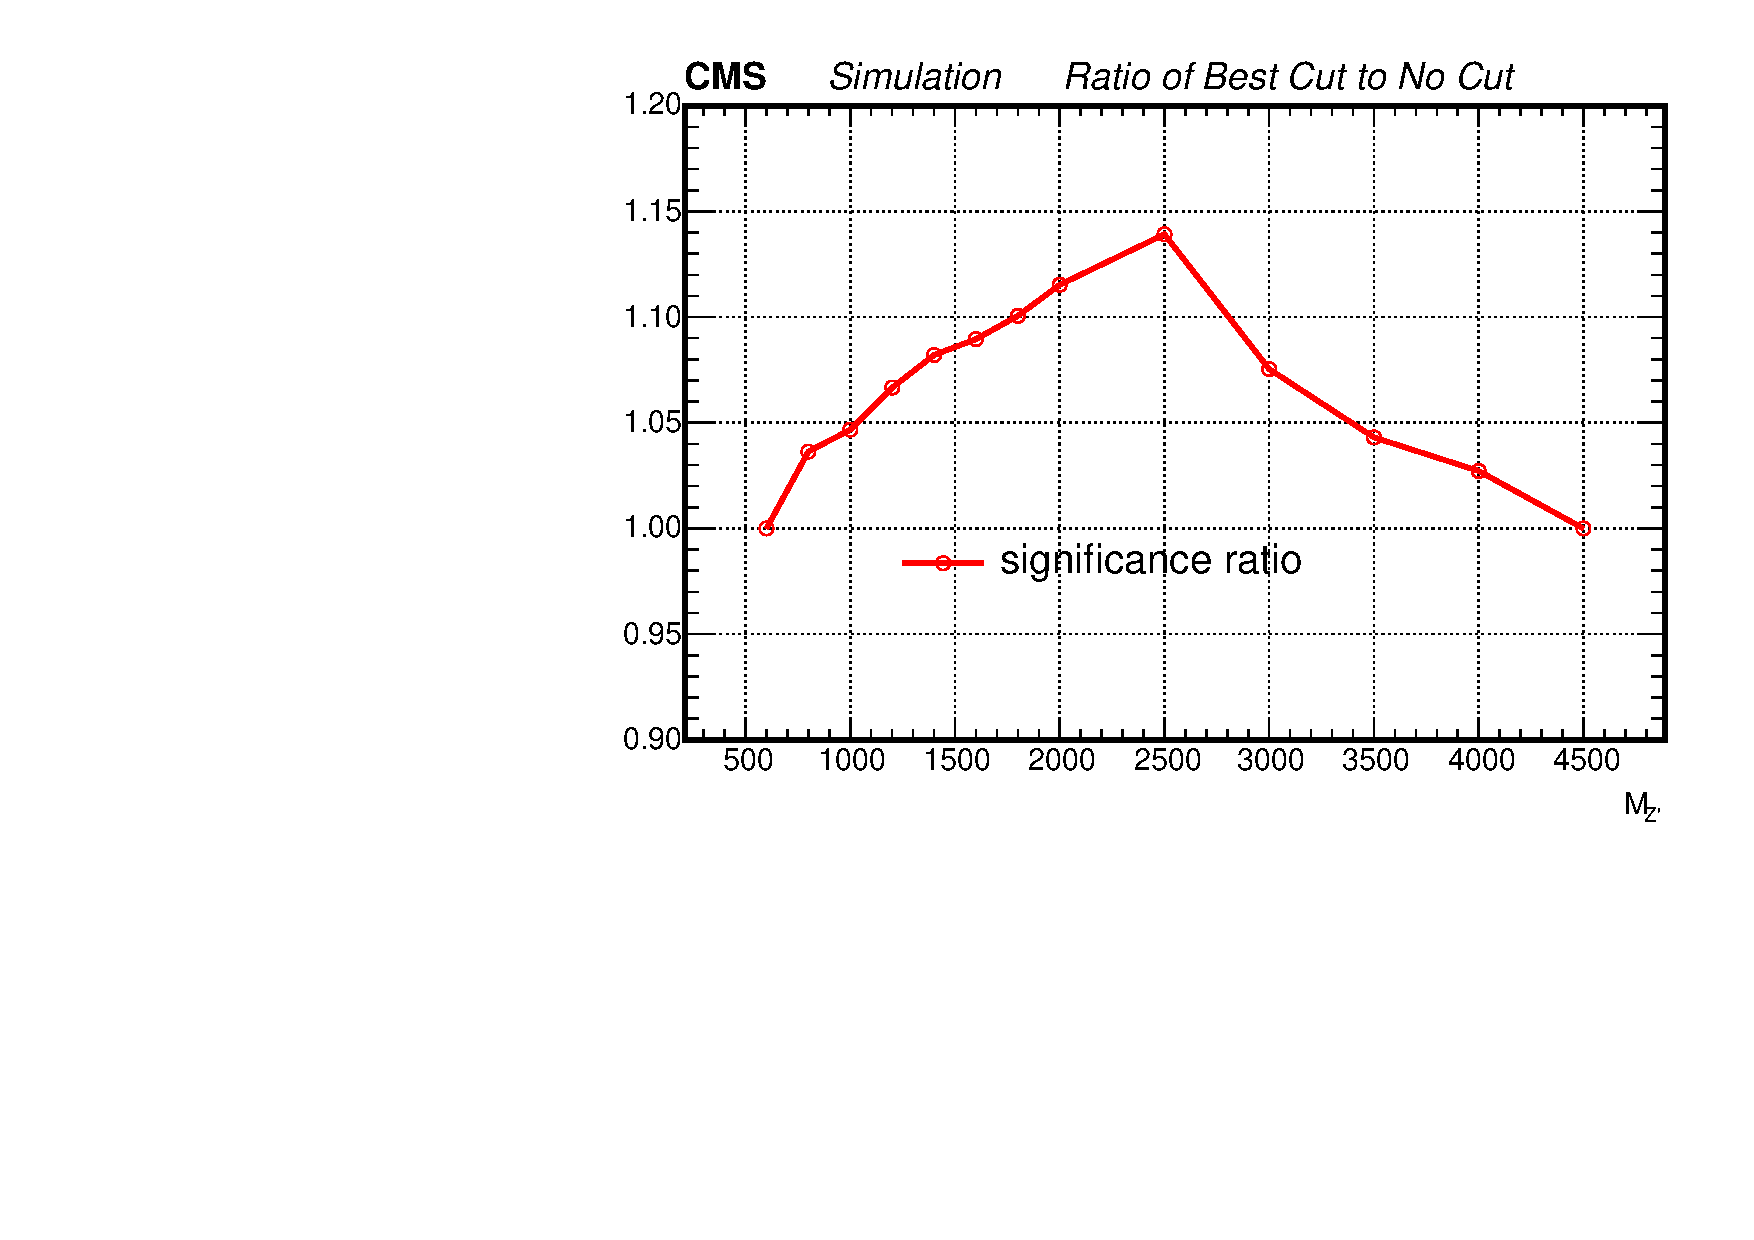
\includegraphics[width=0.45\textwidth]{optimization/plot_1st_pt/plot_1st_pt_significance_ratio_of_best_cut_to_no_cut.pdf}
   \caption{The best Punzi significance for the selection on 
leading electron \pt and the corresponding signal/background 
efficiencies (left), and the ratio of the best significance 
relative to the significance with only preselection (right),  as a function 
of Z' mass. Uncertainties on the efficiencies are binomial.}
  \label{fig:leadptmass}
\end{figure}



%%%%%%%%%%%%%%%%%%%%%%%%%%%%%%%% Subleading electron pt
\begin{figure}[htbp]
   \centering
   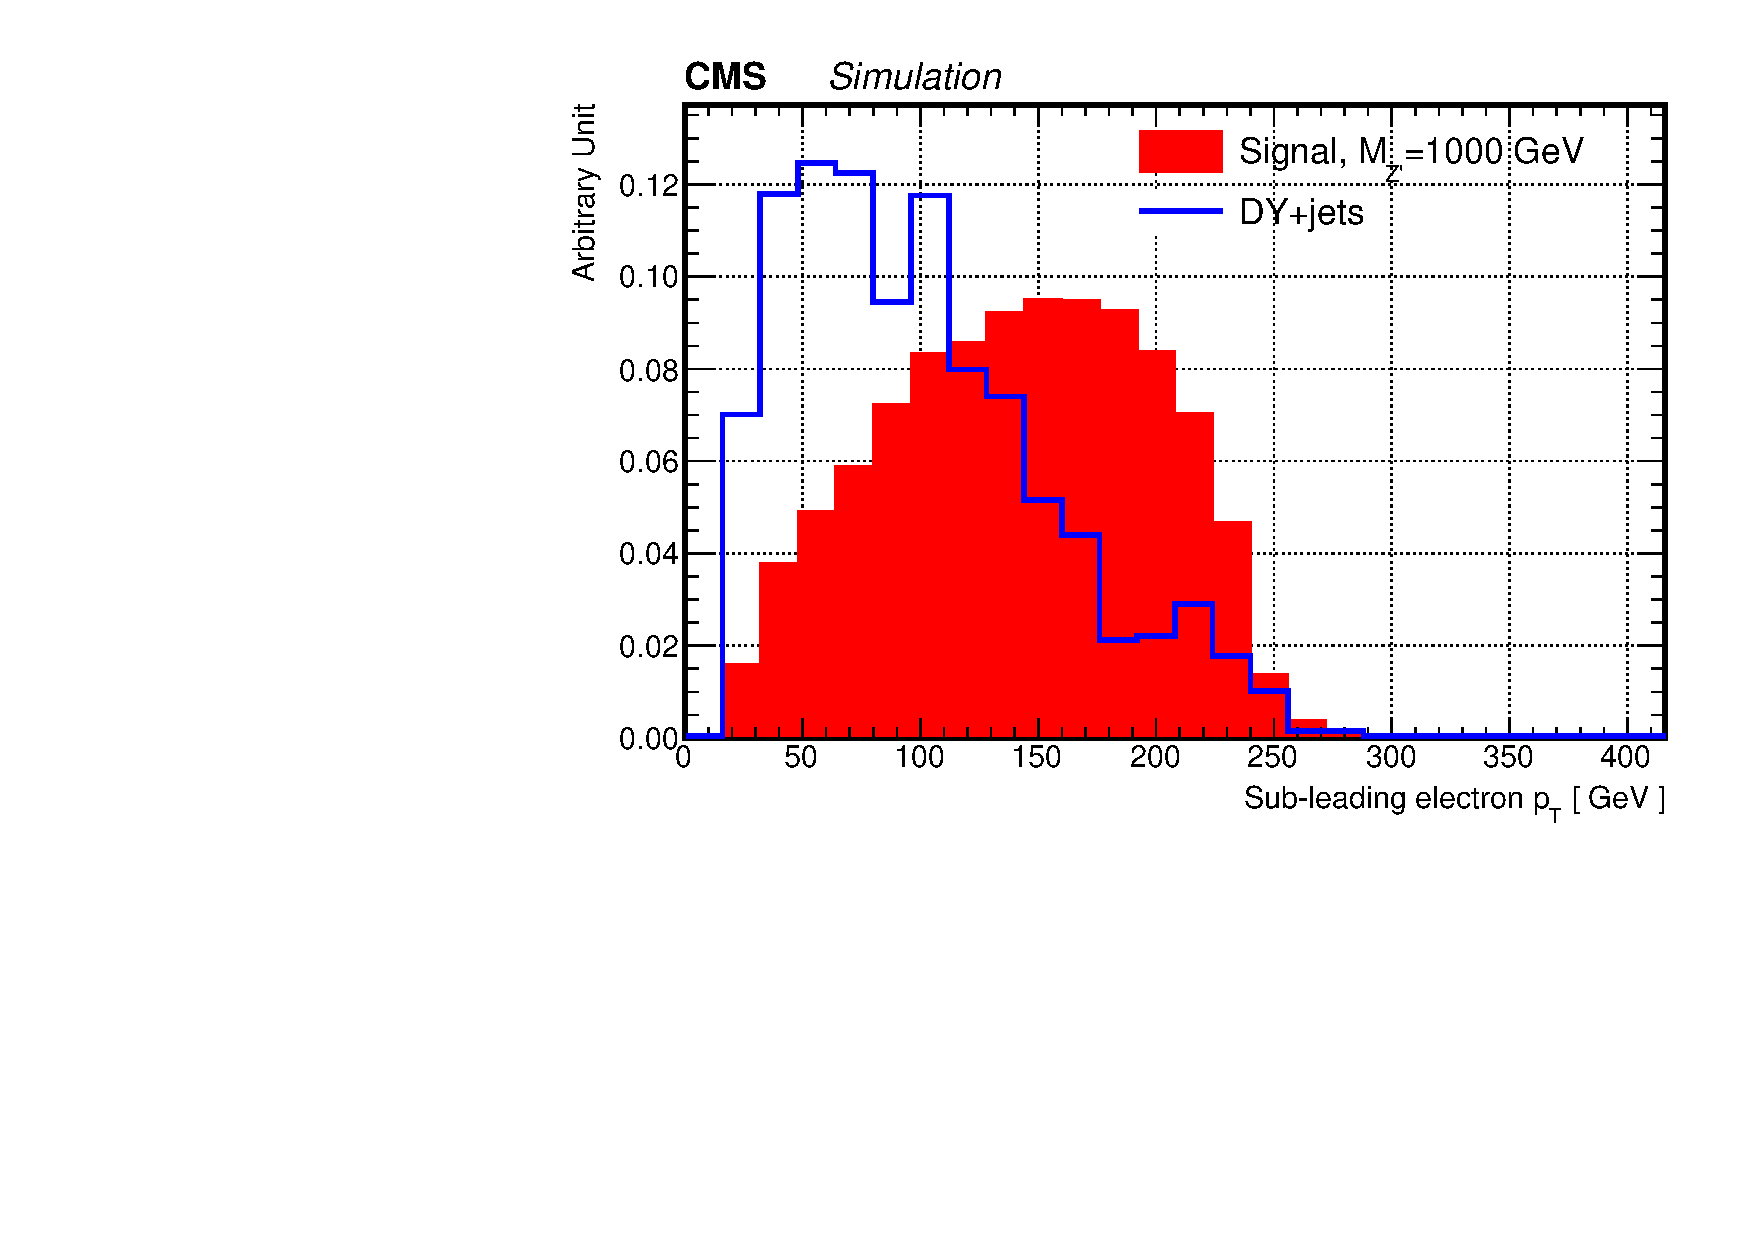
\includegraphics[width=0.45\textwidth]{optimization/plot_2nd_pt/plot_2nd_pt_input_in_Zprime_mass_1000.pdf}
   \includegraphics[width=0.45\textwidth]{optimization/plot_2nd_pt/plot_2nd_pt_Significance_and_efficiency_for_Zprme_M_1000.pdf}
   \caption{The signal and background distributions of sub-leading electron \pt 
(left) and the Punzi significance, the signal, and the background efficiencies as a 
 function of minimum \pt threshold (right). The Z' mass is set to 1 TeV. The 
   signal and background distributions on the left are normalized to the same 
   integrated area. The uncertainties on the right are correlated between 
 different bins.}
   \label{fig:subptone}
\end{figure}

\begin{figure}[htbp]
   \centering
   \includegraphics[width=0.45\textwidth]{optimization/plot_2nd_pt/plot_2nd_pt_input_in_Zprime_mass_2000.pdf}
   \includegraphics[width=0.45\textwidth]{optimization/plot_2nd_pt/plot_2nd_pt_Significance_and_efficiency_for_Zprme_M_2000.pdf}
   \caption{The signal and background distributions of sub-leading electron \pt 
(left) and the Punzi significance, the signal, and the background efficiencies as a 
 function of minimum \pt threshold (right). The Z' mass is set to 2 TeV. The 
   signal and background distributions on the left are normalized to the same 
   integrated area. The uncertainties on the right are correlated between 
 different bins.}
   \label{fig:subpttwo}
\end{figure}

\begin{figure}[htbp]
   \centering
   \includegraphics[width=0.45\textwidth]{optimization/plot_2nd_pt/plot_2nd_pt_input_in_Zprime_mass_3000.pdf}
   \includegraphics[width=0.45\textwidth]{optimization/plot_2nd_pt/plot_2nd_pt_Significance_and_efficiency_for_Zprme_M_3000.pdf}
   \caption{The signal and background distributions of sub-leading electron \pt 
(left) and the Punzi significance, the signal, and the background efficiencies as a 
 function of minimum \pt threshold (right). The Z' mass is set to 3 TeV. The 
   signal and background distributions on the left are normalized to the same 
   integrated area. The uncertainties on the right are correlated between 
 different bins.}
   \label{fig:subptthree}
\end{figure}


\begin{figure}[htbp]
   \centering
   \includegraphics[width=0.45\textwidth]{optimization/plot_2nd_pt/plot_2nd_pt_best_cut_significance_and_efficiency.pdf}
   \includegraphics[width=0.45\textwidth]{optimization/plot_2nd_pt/plot_2nd_pt_significance_ratio_of_best_cut_to_no_cut.pdf}
   \caption{The best Punzi significance for the selection on 
sub-leading electron \pt and the corresponding signal/background 
efficiencies (left), and the ratio of the best significance 
relative to the significance with only preselection (right),  as a function 
of Z' mass. Uncertainties on the efficiencies are binomial.}
  \label{fig:subptmass}
\end{figure}



\subsubsection*{Optimization of selection criteria based on event topology \label{sec:opt_topo}}
 While the \pt's of leading and sub-leading electrons 
strongly depend on the mass of Z' (Appendix~\ref{sec:opt_ele}), several 
kinematic variables have little dependence on the Z' mass and are sensitive to 
the spin of the particles and the squared matrix element. These kinematic 
variables are: 
 \begin{itemize}
 \item $\cos{\theta^*}$, the angle between the momentum of one daughter 
(either higgs or Z here) as measured in the Z' rest frame and the flight 
direction of the Z' in the lab frame (z-axis), a variable sensitive to spin 
of Z' and the squared matrix element 
 \item $\Delta y_{ZH}$, the rapidity difference between the higgs and the 
leptonic-Z, this variable can be approximated by the pseudo-rapidity 
difference $\Delta \eta_{ZH}$, which is related to $\cos{\theta^*}$: 
\[
\cos{\theta^*}=\tanh{\left(\frac{\Delta \eta_{ZH}}{2}\right)}.
\]
 \item $\cos{\theta_{1,2}}$, the angle between the momentum of one daughter of 
higgs (leptonic-Z) as measured in the higgs (leptonic-Z) rest 
frame and the flight direction of the higgs (leptonic-Z) boson in the lab 
frame, a variable sensitive to the spin of higgs (leptonic-Z) and 
the squared matrix element 
 \end{itemize}

Figures~\ref{fig:lheone}--\ref{fig:lhetwo} show the distributions of these 
kinematic variables from Z' mass of 800 GeV to Z' mass of 4500 GeV. Little 
difference is seen between different mass values. 
Figure~\ref{fig:bkgangle} shows the angular distributions 
of the major background DY+jets events. 
The shapes of the signal and the background are similar for the 
$\cos{\theta_{1,2}}$. Nevertheless, the $\cos{\theta^*}$ of the Z' 
signal has a parabola shape (frowny face) with most of the 
events around $\cos{\theta^*}\sim 0$, while the $\cos{\theta^*}$ of 
DY+jets has a shape of smiley face with peaks at 
around $\left|\cos{\theta^*}\right|\sim 1$. 
Given that one could see a distinctive shape difference between signal and 
background in the $\cos{\theta^*}$ distribution, we choose to optimize 
the variable $\Delta \eta_{ZH}$, which is a variable closely related to 
$\cos{\theta^*}$ and is easier to compute\footnote{The pseudorapidity difference 
is smaller for the $s$-channel processes such as the Z' signal model than for 
the $t$-channel processes dominating DY+jets background.}. 

We first find out the best selection criteria by optimizing on the Punzi 
significance as detailed in Appendix~\ref{sec:opt_ele}. 
Figures~\ref{fig:detaone}--\ref{fig:detathree} show (i) the signal and background 
distributions of $\Delta \eta_{ZH}$, and (ii) the Punzi significance, signal and 
background efficiencies as a function of maximum $\Delta \eta_{ZH}$ thresholds, 
for Z' mass at 1, 2, and 3 TeV, respectively. 
Figure~\ref{fig:detamass} shows, as a function of Z' mass, 
(i) the best Punzi significance and its corresponding 
signal/background efficiencies, and (ii) the ratio of best significance relative 
to the significance with preselection only. One 
could see that an additional 1-13\% improvement of significance 
(maximum at $M_{Z'}=$2~TeV) could be gained by applying the 
$\Delta \eta_{ZH}$ selection.
Note that due to the small size of simulated samples, very few background 
events satisfy the preselection, particularly the $M_{Zh}$ requirement. 
For example, only one DY+jets 
background event survives the pre-selection for the optimization at 
$M_{Z'}=$4.5~TeV. 

\begin{figure}[htbp]
   \centering
   \includegraphics[width=0.45\textwidth]{optimization/LHE_study/LHE_XZh_cosThetaStar.pdf}
   \includegraphics[width=0.45\textwidth]{optimization/LHE_study/LHE_XZh_B_dEta.pdf}
   \caption{Comparison of the LHE-level $\cos{\theta^*}$ (left) and 
$\Delta \eta_{ZH}$ (right) for 12 Z' mass values, from 800 GeV to 4500 GeV.}
   \label{fig:lheone}
\end{figure}


\begin{figure}[htbp]
   \centering
   \includegraphics[width=0.45\textwidth]{optimization/LHE_study/LHE_XZh_cosTheta1.pdf}
   \includegraphics[width=0.45\textwidth]{optimization/LHE_study/LHE_XZh_cosTheta2.pdf}
   \caption{Comparison of the LHE-level $\cos{\theta_1}$ (left) and 
$\cos{\theta_2}$ (right) for 12 Z' mass values, from 800 GeV to 4500 GeV. 
The $\cos{\theta_1}$ ($\cos{\theta_2}$) is computed with the four-momentum of 
the higgs (leptonic-Z) daughters.}
   \label{fig:lhetwo}
\end{figure}

\begin{figure}[htbp]
   \centering
   \includegraphics[width=0.3\textwidth]{optimization/LHE_study/angle_cosThetaStar.pdf}
   \includegraphics[width=0.3\textwidth]{optimization/LHE_study/angle_cosTheta1.pdf}
   \includegraphics[width=0.3\textwidth]{optimization/LHE_study/angle_cosTheta2.pdf}
   \caption{The $\cos{\theta^*}$ (left), $\cos{\theta_1}$ (middle) and 
$\cos{\theta_2}$ (right) 
from DY+jets events. }
   \label{fig:bkgangle}
\end{figure}


\begin{figure}[htbp]
   \centering
   \includegraphics[width=0.45\textwidth]{optimization/plot_dEta/plot_dEta_input_in_Zprime_mass_1000.pdf}
   \includegraphics[width=0.45\textwidth]{optimization/plot_dEta/plot_dEta_Significance_and_efficiency_for_Zprme_M_1000.pdf}
   \caption{The signal and background distributions of $\Delta \eta_{ZH}$ 
(left) and the Punzi significance, the signal, and the background efficiencies as a 
function of $\Delta \eta_{ZH}$ 
   selection: $\Delta \eta_{ZH} < x$ (right). The Z' mass is set to 1 TeV. The 
   signal and background distributions on the left are normalized to the same 
   integrated area. The uncertainties on the right are correlated between 
 different bins.}
   \label{fig:detaone}
\end{figure}

\begin{figure}[htbp]
   \centering
   \includegraphics[width=0.45\textwidth]{optimization/plot_dEta/plot_dEta_input_in_Zprime_mass_2000.pdf}
   \includegraphics[width=0.45\textwidth]{optimization/plot_dEta/plot_dEta_Significance_and_efficiency_for_Zprme_M_2000.pdf}
   \caption{The signal and background distributions of $\Delta \eta_{ZH}$ 
(left) and the Punzi significance, the signal, and the background efficiencies as a 
function of $\Delta \eta_{ZH}$ selection: $\Delta \eta_{ZH} < x$ (right). The 
Z' mass is set to 2 TeV. The
   signal and background distributions on the left are normalized to the same
   integrated area. The uncertainties on the right are correlated between 
 different bins.}
   \label{fig:detatwo}
\end{figure}

\begin{figure}[htbp]
   \centering
   \includegraphics[width=0.45\textwidth]{optimization/plot_dEta/plot_dEta_input_in_Zprime_mass_3000.pdf}
   \includegraphics[width=0.45\textwidth]{optimization/plot_dEta/plot_dEta_Significance_and_efficiency_for_Zprme_M_3000.pdf}
   \caption{The signal and background distributions of $\Delta \eta_{ZH}$ 
(left) and the Punzi significance, the signal, and the background efficiencies as a 
     function of $\Delta \eta_{ZH}$ selection: $\Delta \eta_{ZH} < x$ (right). 
     The Z' mass is set to 3 TeV. The signal and background distributions on 
     the left are normalized to the same integrated area. The uncertainties 
on the right are correlated between different bins.}
   \label{fig:detathree}
\end{figure}


\begin{figure}[htbp]
   \centering
   \includegraphics[width=0.45\textwidth]{optimization/plot_dEta/plot_dEta_best_cut_significance_and_efficiency.pdf}
   \includegraphics[width=0.45\textwidth]{optimization/plot_dEta/plot_dEta_significance_ratio_of_best_cut_to_no_cut.pdf}
   \caption{The best Punzi significance for the $\Delta \eta_{ZH}$ selection 
and the corresponding signal/background efficiencies (left), and the ratio 
of the best significance relative to the significance with only preselection 
(right),  as a function of Z' mass. Uncertainties on the efficiencies are 
binomial.}
  \label{fig:detamass}
\end{figure}


\subsubsection*{Higgs-tagging uncertainty}
 An uncertainty of 7\% is associated to the uncertainty on the way to tag a 
Higgs boson. It does not include the \PQb tagging scale factors and the pileup uncertainty. It includes 
the uncertainty due to selection on the pruned mass of the Higgs-jet only. 

The uncertainties on the \PW and top mass tagging are well estimated using 
semileptonic \ttbar sample; the semileptonic \ttbar sample provides a good 
source of boosted hadronic \PW and boosted top. The \PW mass peak in MC 
has been found to be consistent with the mass peak in data 
within statistical uncertainty; the data/MC scale factor is 
$0.992\pm0.005$. On the contrary we have no 
pure source of boosted Higgs. Therefore, we use the following technique to have 
a first estimate of the associated uncertainty. 


We perform a double ratio estimate between bulk graviton going to 
$\PW\PW$ and $\Ph\Ph$. Due to the lack of \HERWIGpp MC samples with HVT models, 
we choose to use the bulk graviton samples for this study. 
%
We choose a mass window for $\PW$ and $\Ph$. We calculate the ratio of 
$\PW$-mass and $\Ph$-mass efficiencies for \PYTHIA and \HERWIG showering algorithms 
and obtain $R_{\HERWIG}$ and $R_{\PYTHIA}$, respectively. Then we calculate 
the double ratio $R_{\HERWIG}/R_{\PYTHIA}$. The 
double ratio provides an estimate how different showering algorithms reacts on 
the difference between \PW~ and \Ph~ decays to jets. 

The values of the double ratios are provided in 
Table~\ref{tab:WideWindow} for \PW~ mass $65 < m_{\PW} <105\GeV$ 
(large window), and Table~\ref{tab:NarrowWindow} for \PW mass 
$65 < m_{\PW} <85\GeV$ (window defined to separate \PW~from \PZz). 
In the first case the difference is approximately of 7\% per jet. While in 
second case a smaller difference of 2\% is observed. One may observe
that the second case corresponds to a more similar efficiency between
$\PW$ and $\Ph$ tagging. 
The source of the difference may be observed in the Fig.~\ref{fig:Masses_PYHG}: 
\HERWIG predicts a larger right tail than \PYTHIA. We verified that this 
difference does not comes from the L2L3 corrections.

Consequently we assign an overall 
uncertainty of 7\% to cover the difference between the potential differences 
between $\PW$ tagging point, where the SF was derived, and $\Ph$ tagging point.

%Finally we vary the jet energy correction to the Higgs tagged jet mass and 
%estimate the change in the normalization.
%This is tabulated in Table~\ref{tab:HiggsMasJESVar}. The effect for each jet 
%is about 3--4\%.


\begin{figure}[h]
\centering
\includegraphics[width=0.48\textwidth]{figures/prunedM_WW-M2000.pdf}
\includegraphics[width=0.48\textwidth]{figures/prunedM_hh-M2000.pdf}\\
\caption{Comparison of \PW (left) and \Ph (right) pruned masses after L2L3 
corrections for \PYTHIA and \HERWIG at $M_\mathrm{bulk}=2~\TeV$.}
\label{fig:Masses_PYHG}
\end{figure}


\begin{sidewaystable}[!htb]
  \begin{center}
\caption{The per-jet efficiency of requiring the mass of Higgs (W) jets to 
be within 105--135 (65--105) \GeV. The efficiency is evaluated with the 
$G_\mathrm{bulk}\rightarrow \mathrm{hh} (\mathrm{WW})$ samples. Each AK8 jet is 
required to match to the generator-level boson within a $\Delta R$ of 0.4. }
  \begin{tabular}{c|rrrrrrr}
\hline\hline
$M_{G_\mathrm{bulk}}$ [GeV] &  $\epsilon_{\mathrm{hh}}^{\HERWIG}$ &  $\epsilon_{\mathrm{WW}}^{\HERWIG}$ & $\epsilon_{\mathrm{hh}}^{\HERWIG}/\epsilon_{\mathrm{WW}}^{\HERWIG}$ 
                                         &  $\epsilon_{\mathrm{hh}}^{\PYTHIA}$ &  $\epsilon_{\mathrm{WW}}^{\PYTHIA}$ &  $\epsilon_{\mathrm{hh}}^{\PYTHIA}/\epsilon_{\mathrm{WW}}^{\PYTHIA}$ &  $R_{\HERWIG}/R_{\PYTHIA}$ \\
\hline

1000 & 0.454 $\pm$ 0.002 & 0.811 $\pm$ 0.003 & 0.559 $\pm$ 0.0028 & 0.494 $\pm$ 0.002 & 0.817 $\pm$ 0.002 & 0.605 $\pm$ 0.0027 & 0.924 $\pm$ 0.0062 \\
2000 & 0.491 $\pm$ 0.002 & 0.792 $\pm$ 0.003 & 0.619 $\pm$ 0.0031 & 0.534 $\pm$ 0.002 & 0.8 $\pm$ 0.002 & 0.667 $\pm$ 0.0028 & 0.928 $\pm$ 0.0061 \\
3000 & 0.462 $\pm$ 0.002 & 0.765 $\pm$ 0.003 & 0.604 $\pm$ 0.0032 & 0.505 $\pm$ 0.002 & 0.774 $\pm$ 0.003 & 0.653 $\pm$ 0.003 & 0.925 $\pm$ 0.0065 \\
\hline
\hline
\end{tabular}
\label{tab:WideWindow}
\end{center}
%\end{sidewaystable}

\vspace{1.2pt}
%\begin{sidewaystable}[!htb]
  \begin{center}
\caption{The per-jet efficiency of requiring the mass of Higgs (W) jets to 
be within 105--135 (65--85) \GeV. The efficiency is evaluated with the 
$G_\mathrm{bulk}\rightarrow \mathrm{hh} (\mathrm{WW})$ samples. Each AK8 jet is 
required to match to the generator-level boson within a $\Delta R$ of 0.4. }
  \begin{tabular}{c|rrrrrrr}
\hline\hline
$M_{G_\mathrm{bulk}}$ [GeV] &  $\epsilon_{\mathrm{hh}}^{\HERWIG}$ &  $\epsilon_{\mathrm{WW}}^{\HERWIG}$ & $\epsilon_{\mathrm{hh}}^{\HERWIG}/\epsilon_{\mathrm{WW}}^{\HERWIG}$ 
                                         &  $\epsilon_{\mathrm{hh}}^{\PYTHIA}$ &  $\epsilon_{\mathrm{WW}}^{\PYTHIA}$ &  $\epsilon_{\mathrm{hh}}^{\PYTHIA}/\epsilon_{\mathrm{WW}}^{\PYTHIA}$ &  $R_{\HERWIG}/R_{\PYTHIA}$ \\
\hline
1000 &   0.454 $\pm$ 0.002 & 0.54 $\pm$ 0.004 & 0.84 $\pm$ 0.0065 & 0.494 $\pm$ 0.002 & 0.581 $\pm$ 0.003 & 0.851 $\pm$ 0.0053 & 0.987 $\pm$ 0.0098 \\  
2000 &   0.491 $\pm$ 0.002 & 0.632 $\pm$ 0.004 & 0.777 $\pm$ 0.0051 & 0.534 $\pm$ 0.002 & 0.674 $\pm$ 0.003 & 0.792 $\pm$ 0.0041 & 0.981 $\pm$ 0.0082 \\
3000 &   0.462 $\pm$ 0.002 & 0.591 $\pm$ 0.004 & 0.781 $\pm$ 0.0055 & 0.505 $\pm$ 0.002 & 0.631 $\pm$ 0.003 & 0.801 $\pm$ 0.0045 & 0.976 $\pm$ 0.0088 \\

\hline
\hline
\end{tabular}
\label{tab:NarrowWindow}
\end{center}
\end{sidewaystable}





\subsubsection*{Results}


Results are obtained from a combined signal and background fit to the unbinned \mVH distribution, based on a profile likelihood. Systematic uncertainties are treated as nuisance parameters and are profiled in the statistical interpretation~\cite{CLS1,CLS2,CMS-NOTE-2011-005,Asymptotic}. The background-only hypothesis is tested against the $\X\to\VH$ signal in the ten categories, and
with no evidence of significant deviations from background expectation, the asymptotic modified frequentist method is used to determine the limit at the 95\% confidence level (CL) on the contribution from signal.


The observed upper limit on the resonance cross section times $\B(\X\to\VH)$ and $\B(\htobb)$, as well as the expected limit and its relative 68\% and 95\% uncertainty bands, are reported as a function of the resonance mass in Fig.~\ref{fig:limit}. The limits are obtained by considering a spin-1 heavy resonance in the narrow-width approximation. %produced via the gluon-gluon fusion process 


%\section{Interpretation}
%\label{sec:interpretation}


%\section{The HVT model}

The result of this study is primarily interpreted in the context of a simplified model with heavy vector bosons ($V^\pm$, $V^0$)~\cite{Pappadopulo2014}.  The model is parametrized in terms of the strength of a new interaction, $g_V$, and the coupling between the Higgs boson or longitudinally polarized SM vector bosons $c_H$, and the coupling with the fermions $c_F$.
%The interaction of the HVT to the SM fields is governed by a new contribution to the Lagrangian:
%\begin{eqnarray}
%\nonumber &&\mathcal{L_V} = -\frac{1}{4} D_\mu V_\nu^a D^\mu V^{\nu a} + \frac{{m_V}^2}{2} V_\mu^a V^{\mu a} \\
%\nonumber &&+ i g_V c_H V_\mu^a H^\dagger \tau^a \bar{D}^\mu H   +   \frac{g^2}{g_V} c_F V_\mu^a \sum_f \bar{f}_L \gamma^\mu \tau^a f_L \\
%&&+ \frac{g_V}{2} c_{VVV} \varepsilon_{abc} V_\mu^a V_\nu^b D^\mu V^{\nu c} + \text{quadrilinear terms}~.
%\end{eqnarray}
%In this study, two specific benchmark scenarios are considered. In model A, mainly realized in weakly-coupled models~\cite{Accomando:2010fz,Schmaltz:2010xr}, $c_H$ and $c_F$ are comparable and $g_V \sim g \sim 1$, $c_H = -g^2/g_V^2$, $c_F \sim 1$.
%The HVT Model B is inspired by composite Higgs model~\cite{Agashe:2007ki,Agashe:2008jb,Agashe:2009bb}, 
The values considered in HVT model~B are $g_V = 3$, $c_H = -1$, and $c_F = 1$. With these parameters, the couplings of the resonance to fermions are suppressed, and those to vector bosons are enhanced~\cite{Pappadopulo2014}.
This scenario is particularly interesting because it predicts signal cross sections on the order of 1-10\fb for resonances up to $2 \sim 3 \TeV$, with branching ratios to vector bosons close to the unity, and thus accessible in $\sqrt{s}=13$~\TeV LHC data. The cross section multiplied by the branching ratios predicted in the benchmark scenario B is superimposed to the exclusion limits in Fig.~\ref{fig:limit}.



\begin{figure}[!htb]\centering
    \includegraphics[width=\cmsFigWidth]{figures/Exclusion_XZh.pdf}
    \includegraphics[width=\cmsFigWidth]{figures/Exclusion_XWh.pdf}
%     \caption{Observed and expected 95\% CL upper limit on $\sigma_\X \times \B(\htobb)$ as a function of \mX for a narrow spin-1 resonance, including all statistical and systematic uncertainties.
%       The green and yellow bands are the ${\pm}1$ and ${\pm}2\sigma$ uncertainty bands on the expected limit.}
    \caption{Observed and expected 95\% CL upper limit on $\sigma_\X \times \B(\X\to\VH) \times \B(\htobb)$ as a function of the resonance mass for a narrow spin-1 resonance, including all statistical and systematic uncertainties, for the $\X\to\Z\h$ (left) and $\X\to\PW\h$ (right) decay channels. The green and yellow bands are the ${\pm}1$ and ${\pm}2$ standard deviation uncertainty bands on the expected limit.}
  \label{fig:limit}
\end{figure}


\subsection{Search for heavy resonances decaying to a pair of Higgs bosons in four b quark final state in proton-proton collisions at $\sqrt{s}=13~\TeV$\label{sec:dihiggs}}

\subsubsection*{Introduction}
In this analysis, the group of Prof.~Shin-Shan Yu has performed optimization of pruned mass selections, number of b-tagged subjets, event topology, study of the 
mass difference between the leading and sub-leading jets, study of the resolution of dihiggs invariant mass, 
and estimation of the systematic uncertainties due to jet energy scales, b-tagging scale factors, H-tagging efficiency. 
We also performed synchronization so to resolve 
the discrepancy between two different b-tagging methods: subjet b-tagging and double b-tagging. In addition, we performed combination of the 8 TeV and 13 TeV high-mass 
dihiggs searches. Given that this analysis is still being reviewed by the CMS Collaboration, we will only describe the items listed above and will not show the final result.


\subsubsection*{Optimization of the mass window for the Higgs-jet}
In order to suppress the QCD background, we require the 
corrected pruned mass of the AK8 jet to be consistent with the mass of 
the Higgs boson. As noted in Section~\ref{sec:neutrino}, the mass of the 
sub-leading jet tends to be lower than that of the leading jet. In addition,  
the correlation between the leading and sub-leading jet mass is found 
to be minimal ($\approx 0.003$ for the signal and $\approx 0.02$ for the 
background). Therefore, we perform one-dimensional optimization separately 
for the leading and sub-leading jets assuming that the two mass variables 
are uncorrelated.  

The chosen figure of merit for the optimization is the Punzi significance, 
which has the advantage to be independent on the signal normalization, and is 
defined as:$$\mathcal{P} = \frac{\varepsilon_S}{1+\sqrt{B}}$$ where 
$\varepsilon_S$ is the signal efficiency and $B$ the number of background 
events. 
Here, the $\varepsilon_S$ is the signal efficiency with its 
denominator being the number of signal events passing the preselection 
criteria in Table~\ref{tab:preselection} and the $B$ is the number of 
background events normalized to 3~\fbinv of integrated luminosity. 

Figure~\ref{fig:leadsubmasscorr} shows the 
L2Relative+L3Absolute-corrected pruned mass of the leading and sub-leading 
AK8 jets from the signal and background events. 
Figure~\ref{fig:sigratiomass} shows the ratio of best significance relative 
to the significance when applying a mass cut of 105-135~\GeV to both leading 
and sub-leading jets (common window of the diboson group); in addition, the 
efficiency ratios are also shown. 
Table~\ref{tab:sigratiomass} lists the input numbers of Punzi significance 
for various mass windows and for bulk graviton mass at 1, 2, 3, and 4 TeV 
respectively.
Overall, about 15--35\% of significance is reduced by using the mass window 
105--135~\GeV. 

\begin{table}[!htb]
  \begin{center}
\caption{Pre-selection for the \Xtohh analysis. \label{tab:preselection}}
  \begin{tabular}{rrl}
\hline\hline
  & Physics Quantity & Cut Value\\
\hline
\hline
 & $|\eta|$ of AK8 jet & $< 2.4$   \\
 &     \pt of AK8 jet & $>200$~\GeV   \\
\hline
\hline
 & $\tau_{21}$ & $<0.75$  \\
 & $\tau_{21}$ of at least one AK8 jet  & $<0.5$  \\
\hline
 \hline
 & $\Delta \eta (j_1,j_2)$ & $<1.3$ \\
 & $M_{jj}$ & $>1$~\TeV \\
 & $M_{jj}$ & $>0.85 \times$ mean \\
\hline
\hline
\multicolumn{3}{c}{Loose $b$-tagging}\\
\hline
when $\Delta R_\mathrm{subjets} < 0.3$ &
 CISVV2$_\mathrm{fatjet}$ & $>0.605$ \\
when $\Delta R_\mathrm{subjets} > 0.3$ &
at least one CISVV2$_\mathrm{subjet}$ & $>0.605$ \\
\hline
\multicolumn{3}{c}{Tight $b$-tagging}\\
\hline
when $\Delta R_\mathrm{subjets} < 0.3$ &
 CISVV2$_\mathrm{fatjet}$ & $>0.605$ \\
when $\Delta R_\mathrm{subjets} > 0.3$ &  
two CISVV2$_\mathrm{subjet}$ & $>0.605$ \\
\hline
Overall & \multicolumn{2}{c}{Tight-Tight or Tight-Loose}\\
\hline\hline
 \end{tabular}
 \end{center}
\end{table}

\begin{figure}[htbp]
   \centering
   \includegraphics[width=0.45\textwidth]{figures/optimization/mass/FATjetPRmassL2L3Corr.pdf}
   \includegraphics[width=0.45\textwidth]{figures/optimization/mass/FATjetPRmassL2L3Corr_2.pdf}
   \caption{The distributions of L2Relative+L3Absolute-corrected 
     pruned mass of the leading (left) and sub-leading (right) jets, 
     from the bulk graviton signals and QCD background events,
     respectively. }
   \label{fig:leadsubmasscorr}
\end{figure}



\begin{figure}[!htb]
  \begin{center}
    \includegraphics[width=.9\textwidth]{figures/optimization/mass/dihiggs_bestWindow_ratio.pdf}
  \end{center}
  \caption{The ratio of the best significance relative to the significance 
 with mass window of 105--135~\GeV,  as a function 
of bulk graviton mass. The corresponding efficiency ratios for the signal 
 and background are also shown. }  
  \label{fig:sigratiomass}
\end{figure}


\begin{table}[!htb]
  \begin{center}
\caption{Punzi significance, the signal efficiency and the number of 
 background events for various mass windows. The numbers in bold font 
 correspond to the mass 
 window with best significance for the \Xtohh analysis. The numbers for the  
 common window 105--135 GeV are also shown. \label{tab:sigratiomass}}
  \begin{tabular}{c|crrr}
 \hline
 \hline
 $M_{G}$ & corr. $M_\mathrm{pruned}$ [\GeV] & $\mathcal{P}$ &  $\varepsilon_S$ & $B$ \\
 \hline
  1 \TeV & {\bf 110--140}, {\bf 110--140} 
                    & {\bf 4.56e-03} & {\bf 0.3838} & {\bf 6906.74} \\ 
         & 105--135, 105--135 &  3.96e-03 & 0.3345 & 6982.58 \\
 \hline
  2 \TeV & {\bf 105--130}, {\bf 95--130} 
                    & {\bf 3.19e-02} & {\bf 0.4404} & {\bf 164.38} \\
         & 105--135, 105--135 & 2.78e-02 & 0.3882 & 168.22 \\
  \hline
  3 \TeV & {\bf 105--130}, {\bf 90--130} 
                    & {\bf 1.22e-01} & {\bf 0.4672} & {\bf 8.028} \\
         & 105--135, 105--135 & 1.20e-01 & 0.3751 & 4.550 \\
  \hline
  4 \TeV & {\bf 105--130}, {\bf 90--130} 
                    & {\bf 2.19e-01} & {\bf 0.4288} & {\bf 0.9263} \\
         & 105--135, 105--135 & 1.79e-01 & 0.3553 & 0.9649 \\
 \hline
 \hline
 \end{tabular}
 \end{center}
\end{table}

\subsubsection*{Optimization of the number of b-tagged subjets \label{sec:optnbsub}}

Our signal contains four b quarks in the final state and naively, one should 
require all four subjets to be b-tagged (CISVV2$_\mathrm{subjet}>0.605$). 
However, the subjet b-tagging algorithm is not efficient when the two 
b quarks from the Higgs boson have very small angular separation, i.e. when 
the mass of the new resonance is large and the Higgs bosons are boosted. 
In addition, the QCD background is expected to fall rapidly as the dijet 
invariant mass increases. In this section, therefore, we study the expected 
limits for 
different requirements on the numbers of b-tagged subjets: 
\begin{itemize}
 \item at least three b-tagged subjets
 \item exactly three b-tagged subjets 
 \item exactly four b-tagged subjets
\end{itemize}

Figures~\ref{fig:fracsubb}--\ref{fig:nsubb} show the fraction of and the 
absolute number of events for each number of b-tagged subjets, respectively, 
after we apply the following pre-selection criteria: 
\begin{itemize}
\item Two AK8 jets each with $|\eta|<2.4$, $\pt>200~\GeV$ and
L2Relative+L3Absolute-corrected pruned mass within the window 105--135~\GeV,
\item $M_{jj} > 1~\TeV$.
\end{itemize}
As in Section~\ref{sec:optdeta}, the histograms of the dijet invariant mass 
are used to obtain the expected limits.  
The resulting expected limits as a function of bulk graviton mass for 
various number of b-tagged subjets are shown in Fig.~\ref{fig:nbsublimit}; 
the combined limits of exactly three and four b-tagged subjets give the best 
result. One could also see that below mass of 2.2 TeV, the combined limits 
are dominated by the events with exactly four b-tagged subjets while 
including the events with three b-tagged subjets improves the limits for mass 
above 2.2 TeV.




\begin{figure}[htbp]
   \centering
   \includegraphics[width=0.9\textwidth]{figures/optimization/numberSubjetBtag/CSVNum.png}
   \caption{The fraction of events for each number of b-tagged 
   subjets from the bulk graviton signals and from the QCD background, 
   respectively.}
   \label{fig:fracsubb}
\end{figure}

\begin{figure}[htbp]
   \centering
   \includegraphics[width=0.9\textwidth]{figures/optimization/numberSubjetBtag/CSVNum2.png}
   \caption{The absolute number of events normalized 
     to 3~\fbinv of integrated luminosity for each number of b-tagged 
   subjets from the bulk graviton signals and from the QCD background, 
   respectively.}
   \label{fig:nsubb}
\end{figure}



\begin{figure}[htbp]
   \centering
   \includegraphics[width=0.95\textwidth]{figures/optimization/numberSubjetBtag/limitofNumCSV.png}
   \caption{The 95\% C.L. expected upper limits on the 
     effective production cross section of bulk graviton, as a function of the mass of 
     bulk graviton, for various requirements on the number of b-tagged 
     subjets.}
   \label{fig:nbsublimit}
\end{figure}


\subsubsection*{Optimization of the maximum $\Delta \eta (j_1,j_2)$ \label{sec:optdeta}}

The maximum threshold value of $\Delta \eta (j_1,j_2)$ in 
Table~\ref{tab:preselection}, 
$\Delta \eta (j_1,j_2)<1.3$, is the value used by the Run 1 
analysis.  
We have re-optimized this selection using the 13 TeV bulk graviton MC after 
applying the following requirement:
\begin{itemize}
\item Two AK8 jets each with $|\eta|<2.4$, $\pt>200~\GeV$ and 
L2Relative+L3Absolute-corrected pruned mass within the window 105--135~\GeV,
\item $M_{jj} > 1~\TeV$.
\end{itemize}

The figure of merit for the optimization is the 95\% C.L. expected upper limit 
on the effective production cross section: 
$\sigma(G_\mathrm{bulk}){\cal B}(G_\mathrm{bulk}\rightarrow \Ph\Ph){\cal B}(\Ph\rightarrow bb){\cal B}(\Ph\rightarrow bb)$. 
The dijet invariant mass spectra are saved in histograms with a bin width of 
5~\GeV, for both the signal and the QCD background, and then passed to 
the Higgs combination tool. 
Figures~\ref{fig:detaOne}--~\ref{fig:detaTwo} show the distributions of 
$\Delta \eta (j_1,j_2)$ for bulk graviton mass at 1, 2, 3, and 4~\TeV, 
respectively. 
Figures~\ref{fig:detaMOne}--~\ref{fig:detaMTwo} show the distributions of 
the dijet invariant mass from the bulk graviton signal and from the QCD background 
after making the preselection and requiring $\Delta \eta (j_1,j_2) < 1.1$, in 
linear and in log scales, respectively. 
The resulting expected limits as a function of bulk graviton mass for various 
maximum $\Delta \eta (j_1,j_2)$ thresholds are shown in Fig.~\ref{fig:detalimit}. 
Overall, we find that the best selection criteria for all mass points is 
$\Delta \eta (j_1,j_2)<1.1$, which is slightly tighter than the value used by 
 the Run 1 analysis.


\begin{figure}[htbp]
   \centering
   \includegraphics[width=0.45\textwidth]{figures/optimization/deta/dEtawithoutMjjCutM1000.pdf}
   \includegraphics[width=0.45\textwidth]{figures/optimization/deta/dEtawithoutMjjCutM2000.pdf}
   \caption{The distributions of $\Delta \eta$ between the two AK8 jets,  
     from the bulk graviton signals with mass of 1~\TeV (left) and 2~\TeV 
     (right) and from the QCD background events, respectively. }
   \label{fig:detaOne}
\end{figure}


\begin{figure}[htbp]
   \centering
   \includegraphics[width=0.45\textwidth]{figures/optimization/deta/dEtawithoutMjjCutM3000.pdf}
   \includegraphics[width=0.45\textwidth]{figures/optimization/deta/dEtawithoutMjjCutM4000.pdf}
   \caption{The distributions of $\Delta \eta$ between the two AK8 jets,  
     from the bulk graviton signals with mass of 3~\TeV (left) and 4~\TeV 
     (right) and from the QCD background events, respectively. }
   \label{fig:detaTwo}
\end{figure}

\begin{figure}[htbp]
   \centering
   \includegraphics[width=0.9\textwidth]{figures/optimization/deta/Mjj_opt_11.png}
   \caption{The distributions of dijet invariant mass, in linear scale, 
     from the bulk graviton signal and from the QCD background events, after
     preselection and requiring $\Delta \eta (j_1,j_2) < 1.1$. }
   \label{fig:detaMOne}
   \includegraphics[width=0.9\textwidth]{figures/optimization/deta/log_Mjj_opt_11.png}
   \caption{The distributions of dijet invariant mass, in log scale, 
     from the bulk graviton signal and from the QCD background events, after
     preselection and requiring $\Delta \eta (j_1,j_2) < 1.1$. }
   \label{fig:detaMTwo}
\end{figure}



\begin{figure}[htbp]
   \centering
   \includegraphics[width=0.95\textwidth]{figures/optimization/deta/shape1.png}
   \caption{The 95\% C.L. expected upper limits on the effective production cross 
     section of bulk graviton, as a function of the mass of 
     bulk graviton, for $\Delta \eta (j_1,j_2)<$0.8--1.5.}
   \label{fig:detalimit}
\end{figure}


\subsubsection*{The contribution of neutrinos within AK8 b-jets \label{sec:neutrino}}

Figure~\ref{fig:leadsubmass} shows, from the bulk graviton signal MC samples, 
the uncorrected\footnote{The pruned and softdrop mass are uncorrected 
but the four-momentum of the jets are corrected with CMS official JEC.}
 mass distributions of the leading\footnote{The sorting of \pt 
is performed with the ungroomed and JEC-applied four-momentum.} and 
sub-leading AK8 b-jets with two different grooming techniques: pruning and 
soft drop. One could see that in both cases the mass of the sub-leading jet 
is about 5~\GeV lower than that of the leading jet. On average, 20-25\% of 
the time, a b-hadron decays semileptonically to a charged lepton, a neutrino, 
and a charm hadron. 
A charm hadron also decays semileptonically, 20-25\% of the time, to a charged 
lepton, a neutrino, and a strange hadron. Therefore, the energy response of a 
heavy flavor jet 
tends to be lower due to the missing neutrino. However, the default Jet Energy 
Calibration (JEC)\footnote{L1 Offset + L2 Relative + L3 Absolute (+L2L3 
Residual) for the MC (data).} does not take into account the difference 
between jet flavors. 
We suspect that the sub-leading b-jet contains more neutrinos, which 
results in a lower \pt and a lower mass for the sub-leading jet. 

In order to study the contribution of neutrinos within the b-jet, we 
first find two leading AK8 jets that satisfy the selection in 
Table~\ref{tab:neutrino}. Then, we look for generator-level neutrinos 
of which the mother is a charm or a b hadron. We obtain the vector-summed 
\pt of all the generator-level neutrinos that are matched to the selected 
AK8 jet within $\Delta R < 0.8$. 
Figure~\ref{fig:neutwo} shows the average of the 
vector-summed generator-level neutrino \pt as a function of the \pt and as a 
function of the pruned mass of the leading and sub-leading jets, for bulk 
graviton signal with mass of 2~TeV. 
One could see that overall the contribution of neutrino, in terms of the 
amount of \pt, is higher in the sub-leading jets with respect to the 
leading jets.

\begin{table}[!htb]
  \begin{center}
\caption{Pre-selection for the study of neutrino contribution within an AK8 b-jet. 
  \label{tab:neutrino}}
  \begin{tabular}{rl}
\hline\hline
  Physics Quantity & Cut Value\\
\hline
\hline
 $|\eta|$ of AK8 jet & $< 2.4$   \\
 \pt of AK8 jet & $>300$~\GeV   \\
 LooseJet ID & true \\ 
 uncorr. M$_\mathrm{pruned}$ & $> 40$~\GeV \\
 CISVV2$_\mathrm{fatjet}$ & 0.605--1.000 \\
\hline\hline
 \end{tabular}
 \end{center}
\end{table}



\begin{figure}[htbp]
   \centering
   \includegraphics[width=0.45\textwidth]{figures/neutrino_study/PRmass.pdf}
   \includegraphics[width=0.45\textwidth]{figures/neutrino_study/SDmass.pdf}
   \caption{The distributions of uncorrected pruned mass (left) and soft-drop 
mass (right) of the leading (solid line) and sub-leading (dashed line) AK8 
b-jets, from bulk graviton signal events with mass at 2 TeV and 3 TeV, 
respectively. Overall, the peak position of the sub-leading jet shifts to a 
lower value, by about 5~\GeV, with respect to that of the leading jet.}
   \label{fig:leadsubmass}
\end{figure}


\begin{figure}[htbp]
   \centering
   \includegraphics[width=0.45\textwidth]{figures/neutrino_study/tprof_neupt_jetpt_2000.pdf}
   \includegraphics[width=0.45\textwidth]{figures/neutrino_study/tprof_neupt_prmass_2000.pdf}
   \caption{The average of the vector-summed neutrino \pt as a function of the \pt (left) 
     and the uncorrected pruned mass (right) of the leading (triangle) and the 
   sub-leading (square/circle) jets, from bulk graviton signal with mass of 
   2~TeV.}
   \label{fig:neutwo}
\end{figure}

\subsubsection*{Mass distribution after the momentum-scaling}
As noted in Section~\ref{sec:neutrino}, the mass of the 
sub-leading jet tends to be lower than that of the leading jet. 
In addition, neither the mass of the leading jet nor the mass of
the sub-leading jet peaks at 125~\GeV. In order to improve 
the resolution of the dihiggs invariant mass spectrum ($M_{jj}$) and 
to increase the separation of signal and background, we have 
studied four different ad-hoc scalings for the momentum 
of AK8 jets. We compare the RMS and the RMS/Mean of the $M_{jj}$ 
spectrum after the momentum scaling, with respect to those before 
the momentum scaling. 
Note, before any momentum scaling, 
the four-momentum of every AK8 jet has been corrected with the 
following CMS official jet energy corrections: L1 Offset + L2 Relative + L3 
Absolute, using the global tag {\sc 74X\_mcRun2\_asymptotic\_v4}.

The four ad-hoc momentum scalings are listed below:
\begin{itemize}
\item $p4_2$ scaled: scale the four-momentum of the sub-leading jet 
 with a factor $R=125/M_\mathrm{corr. pruned}$. Here, $M_\mathrm{corr. pruned}$
is the pruned mass corrected with L2-Relative + L3-Absolute corrections.

\item $p4_{1\&2}$ scaled: scale the four-momenta of both the leading 
 and the sub-leading jets with a factor $R=125/M_\mathrm{corr. pruned}$. 
Here, $M_\mathrm{corr. pruned}$ 
is the pruned mass corrected with L2-Relative + L3-Absolute corrections. 
\item Case 4: scale the four-momenta of both the leading 
 and the sub-leading jets with a factor $R=125/M_\mathrm{ungroomed}$. Here, 
 $M_\mathrm{ungroomed}$ is the mass of AK8 jets before any grooming.
\item Case 5: instead of $M_{jj}$, use the variable 
 \[M_{jj} - (M_\mathrm{ungroomed}^1-125) - (M_\mathrm{ungroomed}^2-125).\] 
Here, $M_\mathrm{ungroomed}^1$ and $M_\mathrm{ungroomed}^2$ are 
the masses of the two Higgs jets before any grooming.
\end{itemize}


Figure~\ref{fig:massresol} shows the mass distributions before any momentum 
scaling and after the four ad-hoc corrections, from the 2-TeV bulk 
graviton signal and from the QCD events. 
Figure~\ref{fig:RMS} and Fig.~\ref{fig:RMSMean} compare the RMS and the 
RMS/Mean from these five different scenarios, respectively, as a function of 
bulk graviton mass. Overall, ``$p4_{1\&2}$ scaled'' and 
``case-5'' corrections have the best performance.


\begin{figure}[htbp]
   \centering
   \includegraphics[width=0.45\textwidth]{figures/scale_mass/allcuts_2000.pdf}
   \includegraphics[width=0.45\textwidth]{figures/scale_mass/allcuts_QCD.pdf}
   \caption{The distributions of $M_{jj}$ before and after the momentum 
     scaling, from the 2-TeV bulk graviton signal events (left) and from 
     the QCD background events (right).}
   \label{fig:massresol}
\end{figure}


\begin{figure}[htbp]
   \centering
   \includegraphics[width=0.9\textwidth]{figures/scale_mass/allcuts_RMS.pdf}
   \caption{The RMS of the $M_{jj}$ spectrum before and after the momentum 
     scaling as a function of bulk graviton mass.}
   \label{fig:RMS}
\end{figure}

\begin{figure}[htbp]
   \centering
   \includegraphics[width=0.9\textwidth]{figures/scale_mass/allcuts_RMS_Outof_Mean.pdf}
   \caption{The RMS of the $M_{jj}$ spectrum relative to the 
     mean of the $M_{jj}$ spectrum before and after the momentum 
     scaling as a function of bulk graviton mass.}
   \label{fig:RMSMean}
\end{figure}



\subsubsection*{Combinations of the 8 TeV and 13 TeV dihiggs searches}

Figure~\ref{fig:combinedhh4b} shows the combination of the 8~\TeV Radion$\rightarrow\Ph\Ph$ with 
the 4b and 2b2$\tau$ final states and of the 13~\TeV Radion$\rightarrow\Ph\Ph$ with the 4b final 
states. The number of common mass points between the  4b and 2b2$\tau$ final states is three. For the 
time being, we only combined for these three mass points. But soon in the future we will 
combine all the other mass points after doing interpolation of the signal shapes.

\begin{figure}[htbp]
   \centering
   \includegraphics[width=0.9\textwidth]{figures/hh_combined.png}
   \caption{The observed limits, as a function of Radion masses, for the 8 TeV and 13 TeV channels separately 
and after combining both to obtain the best limit.}
   \label{fig:combinedhh4b}
\end{figure}


\section{Analysis of the HGC Test Beam Data}
The manpower working on the test beam data includes Prof. Shin-Shan Yu, the postdoc Dr. Vieri Candelise, and the 
Ph.D. student Yu-Hsiang Chang. We collaborated with a CERN postdoc Arabella Martelli and studied the correlation 
between the peak of the readout signal and the input amount of charge (integrated from -40 to +50 ps around the 
peak). After requiring the peak to be greater than 150 ADC counts and requiring that the signal to be within the 
fiducial region, we find a nice correlation between the peak and the integrated charge. The only exception is 
the channel that is known to be bad.
See Fig.~\ref{fig:testbeam_analysis} for the correlation of all the channels we studied.

\begin{figure}[htbp]
   \centering
   \includegraphics[width=0.9\textwidth]{figures/testbeam_analysis.png}
   \caption{The 2-D distributions of integrated amount of charge vs. the peak value of the signal for all readout channels.}
   \label{fig:testbeam_analysis}
\end{figure}




\bibliography{auto_generated}

